\documentclass{gtpart}
\usepackage{amsmath,amssymb,amsthm,stmaryrd}
\usepackage[all]{xy}
\usepackage{tikz}
\usetikzlibrary{shapes,positioning,fit}
\usepackage{enumerate}
\usepackage{tensor}
\usepackage{mathrsfs}
\usepackage{graphicx}
\usepackage{mathtools}
\makeatletter
\let\std@footnotetext\@footnotetext
\usepackage{setspace}
\let\@footnotetext\std@footnotetext
\makeatother
%\doublespacing
\usepackage{hyperref}

\title{The power operation structure on Morava $E$-theory of height 2 at the prime 3}
\author{Yifei Zhu}

\parskip 0.7pc
\parindent 0pt

\newtheorem{thm}{Theorem}
\newtheorem{cor}[thm]{Corollary}
\newtheorem{prop}[thm]{Proposition}
\theoremstyle{definition}
\newtheorem{defn}[thm]{Definition}
\theoremstyle{remark}
\newtheorem{rmk}[thm]{Remark}
\newtheorem{ex}[thm]{Example}
\newtheorem{cau}[thm]{Caution}

\def\co{\colon\thinspace}
\newcommand{\mb}[1]{\mathbb{#1}}
\newcommand{\mf}[1]{\mathfrak{#1}}
\newcommand{\Hom}{\ensuremath{{\rm Hom}}}
\newcommand{\Aut}{{\rm Aut}}
\newcommand{\LT}{{\rm LT}}
\newcommand{\Spec}{{\rm Spec\thinspace}}
\newcommand{\Proj}{{\rm Proj\thinspace}}
\newcommand{\Spf}{{\rm Spf\thinspace}}
\newcommand{\Ell}{{\rm Ell}}
\newcommand{\Sch}{{\rm Sch}}
\newcommand{\cF}{\overline {\mb F}}
\newcommand{\ck}{\overline k}
\newcommand{\CA}{{\cal A}}
\newcommand{\CB}{{\cal B}}
\newcommand{\CC}{{\cal C}}
\newcommand{\CF}{{\cal F}}
\newcommand{\CG}{{\cal G}}
\newcommand{\CHom}{{\cal H}om}
\newcommand{\CLie}{{\cal L}ie}
\newcommand{\CM}{{\cal M}}
\newcommand{\CO}{{\cal O}}
\newcommand{\CP}{{\cal P}}
\newcommand{\CS}{{\cal S}}
\newcommand{\Mod}{{\rm Mod}}
\newcommand{\Alg}{{\rm Alg}}
\newcommand{\dl}{{\rm DL}}
\newcommand{\Set}{{\rm Set}}
\newcommand{\Sq}{{\rm Sq}}
\newcommand{\Frob}{{\rm Frob}}
\newcommand{\DF}{{{\rm DefFrob}_\BG}}
\newcommand{\Model}{{\rm Model}}
\newcommand{\HGa}{{\widehat{\mb G}_a}}
\newcommand{\HGm}{{\widehat{\mb G}_m}}
\newcommand{\Gm}{{{\mb G}_m}}
\newcommand{\DL}{Dyer-Lashof~}
\newcommand{\EM}{Eilenberg-Mac~Lane~}
\newcommand{\BC}{{\mb C}}
\newcommand{\BE}{{\mb E}}
\newcommand{\BF}{{\mb F}}
\newcommand{\BG}{{\mb G}}
\newcommand{\BN}{{\mb N}}
\newcommand{\BP}{{\mb P}}
\newcommand{\BQ}{{\mb Q}}
\newcommand{\BR}{{\mb R}}
\newcommand{\BW}{{\mb W}}
\newcommand{\BZ}{{\mb Z}}
\newcommand{\fm}{{\mf m}}
\newcommand{\HC}{\widehat{C~}\!}
\newcommand{\HE}{\widehat{E~}\!}
\newcommand{\Hf}{\widehat{f}}
\newcommand{\Hphi}{\widehat{\phi}}
\newcommand{\Hpsi}{\widehat{\psi}}
\newcommand{\HS}{\widehat{S~}\!}
\newcommand{\TA}{\tilde{\A}}
\newcommand{\Tc}{\tilde{c}}
\newcommand{\Tf}{\widetilde{f}}
\newcommand{\Tp}{\widetilde{\psi}}
\newcommand{\TW}{\widetilde{W\thinspace}\!}
\newcommand{\md}{~~{\rm mod}~}
\newcommand{\ad}{{\rm and}}
\newcommand{\HT}{{\rm ht}}
\newcommand{\id}{{\rm id}}
\newcommand{\op}{{\rm op}}
\newcommand{\tf}{{\rm tf}}
\newcommand{\tr}{{\rm trace}}
\newcommand{\univ}{{\rm univ}}
\newcommand{\A}{\alpha}
\newcommand{\G}{\Gamma}
\newcommand{\g}{\gamma}
\newcommand{\K}{\kappa}
\newcommand{\T}{\tau}
\newcommand{\om}{\underline{\omega\!}_{~E/S}}
\newcommand{\p}{\psi^3}
\newcommand{\s}{S^\bullet}
\newcommand{\ce}{\coloneqq}
\newcommand{\isog}[1]{Proposition \ref{prop:isog}\thinspace \eqref{isog(#1)}}
\newcommand{\q}[1]{Proposition \ref{prop:Q}\thinspace \eqref{Q(#1)}}
\newcommand{\go}[1]{Definition \ref{def:go}\thinspace \eqref{go(#1)}}

\numberwithin{equation}{section}
\renewcommand{\theequation}{\thesection.\arabic{equation}}
\numberwithin{thm}{section}

%spelling
%label
%newcommand
%single word / page break
%line break / end space


\begin{document}
\begin{abstract}
 \DL theories organize power operations in cohomology.  We give an 
 overview of the structure of the \DL theories associated to Morava 
 $E$-theories.  When the $E$-theory is an elliptic cohomology theory, 
 this structure enables us to compute power operations by doing 
 calculations with elliptic curves.  We give explicit computations of 
 the \DL theory for a specific $E$-theory spectrum and its 
 $K(1)$-localization.  
\end{abstract}

\maketitle

\tableofcontents

\newpage
\section{Introduction}

\subsection{Motivation}
\label{subsec:mot}

Algebraic topology is a field that solves topological or geometric 
problems by translating them into algebra.  The problem of vector fields 
on spheres asks: What is the maximum integer $k(n)$ for which there 
exist $k$ continuous vector fields on the unit sphere in Euclidean 
$n$-space, linearly independent everywhere?  This was solved by Adams 
\cite{adamsvector} as a classic application of algebraic topology to 
geometry.  The solution was built upon the study of cohomology 
operations---the work of Steenrod and Whitehead \cite{steenrodwhitehead} 
which used the Steenrod squares to study the same problem, and Adams' 
original attempt to replace the Steenrod squares by ``cohomology 
operations of higher kinds.''\footnote{Cf.~\cite[Section 2]{adamsvector}.  
Adams used secondary cohomology operations to solve the Hopf invariant 
one problem \cite{adamshopf}.  }  These led to the construction of the 
Adams operations which were the key tool for solving the vector-field 
problem for spheres.  

The Steenrod squares and the Adams operations are operations in ordinary 
cohomology with $\BZ/2$-coefficients and in $K$-theory respectively, and 
both are examples of an important family of cohomology operations called 
{\em power operations}.  Foundational work on the Steenrod operations 
and the {\em Steenrod algebra} $A^*$ established a model for studying 
power operations in other cohomology theories, as encapsulated in 
\cite[Section 1]{blind}: ``Steenrod constructed a family of elements of 
$A^*$, \ldots \cite{steenrod}, Adem found some relations between them 
\cite{adem}, Serre showed that Steenrod's elements generated $A^*$ and 
Adem's relations implied all relations \cite{serre} and Milnor 
elucidated the full structure of $A^*$ \cite{milnor}.  Nonetheless much 
remains to be understood about $A^*$ and it is an active area of 
research.''  

Following earlier work for ordinary cohomology and $K$-theory, the study 
of power operations for other cohomology theories has been carried out 
by tom Dieck and Quillen for complex cobordism 
\cite{tomdieck, quillenmu}, by McClure for $p$-adic $K$-theory 
\cite{mcclure, H_infty}, by Voevodsky for motivic cohomology \cite{V}, 
and by Ando, Hopkins, and Strickland for Morava $E$-theories 
\cite{AHS04}, among others.  In particular, complex cobordism, $p$-adic 
$K$-theory, and Morava $E$-theories, together with ordinary cohomology, 
all fit into {\em the chromatic filtration}, an organizing principle for 
understanding large-scale phenomena in modern stable homotopy theory 
(cf.~\cite{quillenfgl, orange, tafoverview}).  Under this framework, 
cohomology theories are organized according to the {\em heights} of 
their associated {\em formal group laws}, and also prime by prime: 
ordinary cohomology with rational coefficients at height 0, $p$-adic 
$K$-theory at height 1, complex cobordism and ordinary cohomology with 
$\BZ/p$-coefficients at height $\infty$, and Morava $E$-theories as a 
family of cohomology theories at height $n$ for each $n$---with $n = 2$ 
including elliptic cohomology theories 
\cite{morava, hopkinsmahowald, survey}---and at all primes.  The 
chromatic filtration has an intimate connection with algebraic geometry 
and number theory, and studying power operations from this viewpoint 
brings in new tools and insight from beyond the range of classical 
algebraic topology.  

In elliptic cohomology, the study of power operations is aided by a 
``bridge'' connecting homotopy theory and the theory of elliptic curves 
(see \cite[Theorem B]{cong} and \cite[Theorem 2.9.1]{KM}), and is based 
on work of Ando, Hopkins, and Strickland for the case of supersingular 
curves (see \cite{AHS04}), and work of Ando and Ganter for the case of 
the Tate curve (see \cite{Ando00, ganter}).  Thanks to the 
correspondence across this bridge, explicit constructions and 
computations for power operations flow from calculations with isogenies 
of elliptic curves (cf.~\cite{h2p2}).  With concrete formulas, we hope 
to study the structure underlying power operations in elliptic 
cohomology, along the lines of understanding the Steenrod algebra $A^*$ 
for ordinary cohomology.  Moreover, as explained at the beginning of 
\cite{Ando95}, we hope to learn about the conjectural geometric 
interpretation of Morava $E$-theories (at height $n = 2$) by examining 
power operations, analogous to vector bundles and representation theory 
as encoded in the Adams operations for $K$-theory 
(cf.~\cite{adamsvector, atiyah} and see Example \ref{ex:KU} for details).  


\subsection{Statement of results}
\label{subsec:res}

\subsubsection*{The power operation structure on Morava $E$-theory of height 2 at the prime 3}

Let $p$ be a prime, and $q$ be a power of $p$.  We use the symbols 
$\BF_q$ and $\BZ_q$ to denote a field with $q$ elements and the ring of 
$p$-typical Witt vectors over $\BF_q$ respectively.  In particular 
$\BZ_p$ is the ring of $p$-adic integers.  

For a Morava $E$-theory, the analog of the Steenrod algebra in ordinary 
cohomology is the {\em \DL algebra} as the collection of all power 
operations.  In \cite{h2p2} Rezk explicitly computes the \DL algebra for 
a specific $E$-theory of height 2 at the prime 2.  Following his work, 
at height 2 for the prime 3, we study the power operation structure on 
an $E$-theory $E$ with homotopy groups 
\[
 \pi_* E = E_* \cong \BZ_9 \llbracket h \rrbracket [u^{\pm 1}] 
\]
where $h$ and $u$ are in degrees 0 and 2 respectively.  

As in \cite{h2p2}, our computation of power operations follows the 
approach of \cite{steenrod}: one first defines a total power operation, 
and then uses the computation of the cohomology of the classifying space 
$B\Sigma_m$ for the symmetric group $\Sigma_m$ to obtain individual 
power operations.  By doing calculations with elliptic curves associated 
to $E$, we get formulas for a total power operation $\p$ on $E_0$ and a 
ring $S_3$ which represents a corresponding moduli problem.  Based on 
the computation of $E^* B\Sigma_m$ in \cite{Str98} as reflected in the 
formula for $S_3$, we then define individual power operations $Q_k$, and 
derive the relations they satisfy---action on scalars, additivity, 
commutation relations, Adem relations, Cartan formulas, and the 
Frobenius congruence (see Proposition \ref{prop:Q}).  In view of the 
general structures studied in \cite{cong}, we get an explicit 
description of the corresponding \DL algebra $\G$ as below.  

\begin{defn}[Definition \ref{def:go}]
\label{def}
 \mbox{}
 \begin{enumerate}[(i)]
  \item \label{gamma} Let $i$ be an element generating $\BZ_9$ over 
  $\BZ_3$ with $i^2 = -1$.  Define $\G$ to be the associative ring 
  generated over $\BZ_9 \llbracket h \rrbracket$ by elements $Q_0$, 
  $Q_1$, $Q_2$, and $Q_3$ subject to the following relations: the 
  $Q_k$'s commute with elements in 
  $\BZ_3 \subset \BZ_9 \llbracket h \rrbracket$, and satisfy 
  {\em commutation relations} 
  \begin{equation*}
  \begin{split}
   Q_0 h = & ~ (h^3 - 27 h^2 + 201 h - 342) Q_0 + (3 h^2 - 54 h + 171) Q_1 + (9 h - 81) Q_2 \\
           & + 24 Q_3, \\
   Q_1 h = & ~ (-6 h^2 + 108 h - 334) Q_0 + (-18 h + 171) Q_1 + (-72) Q_2 + (h - 9) Q_3, \\
   Q_2 h = & ~ (3 h - 27) Q_0 + 8 Q_1 + 9 Q_2 + (-24) Q_3, \\
   Q_3 h = & ~ (h^2 - 18 h + 57) Q_0 + (3 h - 27) Q_1 + 8 Q_2 + 9 Q_3, \\
   Q_k i ~ = & ~ (-i) Q_k \text{~for all~} k, 
  \end{split}
  \end{equation*}
  and {\em Adem relations} 
  \begin{equation*}
  \begin{split}
   Q_1Q_0 = & ~ (-6) Q_0Q_1 + 3 Q_2Q_1 + (6 h - 54) Q_0Q_2 + 18 Q_1Q_2 + (-9) Q_3Q_2 \\
            & + (-6 h^2 + 108 h - 369) Q_0Q_3 + (-18 h + 162) Q_1Q_3 + (-54) Q_2Q_3, ~ \\
   Q_2Q_0 = & ~ 3 Q_3Q_1 + (-3) Q_0Q_2 + (3 h - 27) Q_0Q_3 + 9 Q_1Q_3, \\
   Q_3Q_0 = & ~ Q_0Q_1 + (-h + 9) Q_0Q_2 + (-3) Q_1Q_2 + (h^2 - 18 h + 63) Q_0Q_3 \\
            & + (3 h - 27) Q_1Q_3 + 9 Q_2Q_3.  
  \end{split}
  \end{equation*}

  \item \label{omega} Write $\omega \coloneqq \pi_2 E$ which is the 
  kernel of $E^0 S^2 \to E^0$ with 
  $E^0 S^2 \cong \BZ_9 \llbracket h \rrbracket [u] / (u^2)$.  Define 
  $\omega$ as a left $\G$-module with one generator $u$ by 
  \[
   Q_k \cdot u \ce \left\{
   \begin{array}{ll}
     u,  & \quad {\rm if}~k = 1, \\
     0,  & \quad {\rm if}~k \neq 1.  
   \end{array}
   \right.
  \]
 \end{enumerate}
\end{defn}

Our computation is motivated by and based on Rezk's result 
\cite{slides, cong} on the general pattern of power operations for 
Morava $E$-theory spectra.  The formulas in Definition \ref{def} give 
the following concrete version of his theorem, at height 2 for the prime 
3.  (See Section \ref{subsec:DL_E} for details about the notation and 
terminology.)  

\begin{thm}[Theorem \ref{thm:gamma}]
 Let $A$ be a $K(2)$-local commutative $E$-algebra.  Let $\G$ be the 
 graded twisted bialgebra over $E_0$ in Definition 
 \ref{def}\thinspace \eqref{gamma}, and $\omega$ be the $\G$-module in 
 Definition \ref{def} \eqref{omega}.  Then $A_*$ is an $\omega$-twisted 
 $\BZ/2$-graded amplified $\G$-ring.  In particular, for $d \geq 0$, 
 \[
  \pi_* L_{K(2)} \BP_E (\Sigma^d E) \cong \big( R_d \big)_{(3,h)}^\wedge 
 \]
 where $R_d$ is the free $\omega$-twisted $\BZ/2$-graded amplified 
 $\G$-ring with one generator in degree $d$.  
\end{thm}

\subsubsection*{Power operations on the $K(1)$-localization}

On the $K(1)$-localization $F$ of our Morava $E$-theory $E$, the power 
operation structure is simpler: the \DL algebra has a single generator 
$\p_F$ over the ring 
\[
 F_0 = \BZ_9 \llbracket h \rrbracket [h^{-1}]_3^\wedge = 
 \left.\left\{\sum_{n = -\infty}^{\infty} k_n h^n~\right|~k_n \in \BZ_9, 
 \lim_{n \to -\infty} k_n = 0\right\}.  
\]
We derive formulas for this $K(1)$-local power operation $\p_F$ from the 
calculations for the total power operation $\p$ above.  Based on 
\cite[Sections 2.4 and 8.2]{level3}, it boils down to interpreting the 
$K(1)$-local power operations in terms of the elliptic curve and formal 
group data related to our construction of $\p$.  Here are the formulas.  

\begin{prop}[cf.~Corollary \ref{cor:psi3} and Section \ref{subsec:K(1)po}]
 The total power operation 
 \[
  \p \co E^0 \to E^0 [\A] \big/ \big( w(\A) \big) 
 \]
 is given by 
 \begin{equation*}
 \begin{split}
  \p(h) = & ~ h^3 + (\A^3 - 6 \A - 27) h^2 + 3 (-6 \A^3 + \A^2 + 36 \A + 67) h \\
          & + 57 \A^3 - 27 \A^2 - 334 \A - 342, \\
  \p(i) \thinspace = & -i, 
 \end{split}
 \end{equation*}
 where 
 \[
  \A \equiv 0 \md 3 \qquad \ad \qquad 
  w(\A) = \A^4 - 6 \A^2 + (h - 9) \A - 3.  
 \]
 Correspondingly the power operation $\p_F \co F^0 \to F^0$ is given by 
 \begin{equation*}
 \begin{split}
  \psi_F^3(h) = & ~ h^3 - 27 h^2 + 183 h - 180 + 186 h^{-1} + 1674 h^{-2} + (\text{lower-order terms}), \\
  \psi_F^3(i) \thinspace = & -i.  
 \end{split}
 \end{equation*}
\end{prop}


\subsection{Outline of the thesis}

As explained in Section \ref{subsec:mot}, our computational results 
stated in Section \ref{subsec:res} are made possible by the ``bridge'' 
between homotopy theory and the theory of elliptic curves, with power 
operations corresponding to deformations of Frobenius isogenies.  Thus 
naturally this thesis consists of two parts: on one side of the bridge, 
the discussions in Sections \ref{sec:po} and \ref{sec:fg} lead to the 
structure of power operations in Morava $E$-theories; on the other side, 
the topics in Section \ref{sec:ec} are centered around cyclic isogenies 
of elliptic curves.  Finally, in Section \ref{sec:p3}, the bridge 
connects the two sides, and we get an explicit description of the power 
operation structure on Morava $E$-theory at height 2 for the prime 3.  

More details for each section are as follows.  

In Section \ref{sec:po}, we introduce the general theory of power 
operations for cohomology theories represented by commutative ring 
spectra.  Section \ref{subsec:arise} begins with an intuitive 
description of the power operation construction, with power operations 
in $K$-theory as an example, and then discusses the construction 
systematically using the functors of extended powers.  Based on the 
structure of the extended powers, Section \ref{subsec:fit} introduces 
the organizing principle of algebraic theories for power operations, in 
particular, the \DL theory associated to a commutative ring spectrum $R$ 
which models all homotopy operations on commutative $R$-algebra spectra.  

In Section \ref{sec:fg}, we discuss the theory of power operations for 
Morava $E$-theories, specifically, the foundational connection to 
deformations of Frobenius isogenies.  Section \ref{subsec:E} introduces 
Morava $E$-theories in the context of the chromatic filtration which 
relates stable homotopy theory and one-dimensional commutative formal 
groups.  Section \ref{subsec:DL_E} describes the general pattern of 
power operations in any Morava $E$-theory $E$.  Section 
\ref{subsec:bridge} translates from the $E$-\DL theory and related 
categories to categories arising from the formal group and its finite 
flat subgroups associated to $E$, and Section \ref{subsec:subgp} 
describes the structure within the latter categories.  

In Section \ref{sec:ec}, we present some of the basics about elliptic 
curves that are relevant to our computations, and illustrate the theory 
by a specific example built through each subsection.  Section 
\ref{subsec:gp} discusses Weierstrass equations, rigidity, dual 
isogenies, and the group law algorithm.  Section \ref{subsec:tors} 
discusses the structure of torsion subgroups and division polynomials, 
and contains one of our main calculations (Proposition \ref{prop:tors}).  
Section \ref{subsec:fg} discusses $p$-divisible groups, the Serre-Tate 
theorem on deformation theory, and the Hasse invariant and supersingular 
elliptic curves.  Section \ref{subsec:isog} discusses cyclic isogenies 
(with another main calculation in Proposition \ref{prop:isog}) and their 
compositions, the Lubin isogeny construction, and V\'elu's formulas.  
Section \ref{subsec:mp} introduces basic moduli problems for elliptic 
curves, discusses their representability and morphisms, and presents 
examples of how the representing moduli schemes look and how they behave 
under morphisms; in particular, via the Serre-Tate theorem, we produce a 
Morava $E$-theory spectrum in Example \ref{ex:E}.  

In Section \ref{sec:p3}, we connect the calculations with elliptic 
curves in Section \ref{sec:ec} to the theory of power operations in 
Sections \ref{sec:po} and \ref{sec:fg}.  Section \ref{subsec:summary} 
recapitulates our main example developed in Section \ref{sec:ec}, and 
collects the calculations scattered therein.  Section 
\ref{subsec:K(2)po} gives formulas for the total power operation $\p$, 
and then defines the individual power operations $Q_k$ and derives the 
relations they satisfy.  Based on these formulas, Section 
\ref{subsec:K(2)DL} gives an explicit description of the \DL theory in 
terms of an associative ring generated by the $Q_k$'s.  Section 
\ref{subsec:K(1)po} discusses the relationship between the total power 
operation $\p$, at height 2, and the corresponding $K(1)$-local power 
operations, and derives formulas for the latter from the calculations in 
Section \ref{subsec:K(2)po}.  


\subsection{Acknowledgements}

I thank Charles Rezk for his encouragement on this work, and for his 
observation \eqref{charles} which led to Proposition \ref{prop:frob^2}, 
Corollary \ref{cor:K'}, and eventually an approach to Adem relations as 
in the proof of \q{iv}.  

I thank Kyle Ormsby for helpful discussions on the calculations in 
Section \ref{sec:ec}, and for directing me to places in the literature, 
including \cite{kohel}.  The computation in Example \ref{ex:velu} is out 
of his suggestion.  

I thank Tyler Lawson for the sustained support from him I received as a 
student.  


\subsection{Conventions}

All formal groups mentioned in this thesis will be commutative and 
one-dimensional.  

Let $p$ be a prime, and $q$ a power of $p$.  We use the following list 
of symbols.  

\begin{center}
\begin{tabular}{ll}
 $\BZ_{(p)}$ & the localization of $\BZ$ with respect to the ideal $(p)$ \\
 $\BF_q$ & a field with $q$ elements \\
 $\BZ_q$ & the ring of $p$-typical Witt vectors over $\BF_q$ \\
 $\BQ_q$ & the fraction field of $\BZ_q$ \\
 $\BW(k)$ & the ring of $p$-typical Witt vectors over a perfect field $k$ of characteristic $p$ \\
 $\BZ/m$ & the additive group of integers modulo $m$ \\
 $\Sigma_m$ & the symmetric group on $m$ letters \\
 $R^\times$ & the group of units of a ring $R$ \\
 $R_I^\wedge$ & the completion of a ring $R$ with respect to an ideal $I$ \\
 $R\llbracket x \rrbracket$ & the ring of formal power series over a ring $R$ in a variable $x$ \\
 $R (\!(x)\!)$ & the ring of formal Laurent series over a ring $R$ in a variable $x$ \\
 $[n]$ & the multiplication-by-$n$ map on a group scheme \\
       & (and also the induced map on the coordinate ring) \\
 $G[n]$ & the kernel of $[n]$ on a group scheme $G$ \\
 $\underline{\BZ/m}$ & the constant group scheme associated to $\BZ/m$ \\
 $\mu_m$ & the group scheme of $m$'th roots of unity, \\
         & i.e., the kernel of $[m]$ on the multiplicative group scheme \\
 $\HE$ & the formal completion of an elliptic curve $E$ at the identity \\
 $\Set$ & the category of sets \\
 $\Sch$ & the category of schemes \\
 $\Sch/S$ & the category of schemes over a scheme $S$ \\
\end{tabular}
\end{center}


\section{Extended powers and power operations}
\label{sec:po}

\subsection{How a power operation arises}
\label{subsec:arise}

Let $h^*(-)$ be a multiplicative cohomology theory, so that we have maps 
\[
 h^c(X) \otimes h^d(X) \longrightarrow h^{c+d}(X) 
\]
for spaces $X$ and integers $c$ and $d$.  In particular, for each 
$m \geq 0$, we have the $m$'th-power map 
\begin{equation*}
\begin{split}
 h^d(X) \longrightarrow & ~ h^{md}(X) \\
 a ~ \mapsto \thinspace & ~ a^m.  
\end{split}
\end{equation*}
As we will see below, if $h^*(-)$ is represented by a structured 
commutative ring spectrum, the $m$'th-power map lifts to a map $P^m$, 
called {\em the $m$'th total power operation}, fitting into the diagram 
\begin{equation}
\label{relFrob1}
 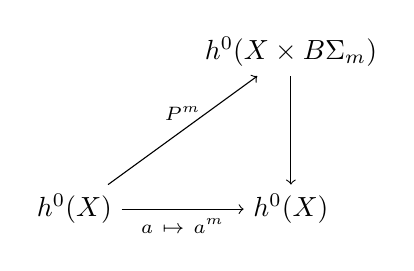
\begin{tikzpicture}[baseline=(current bounding box.center)]
         \node (RT) at (4.65, 2) {$h^0(X \times B\Sigma_m)$}; 
         \node (LB) at (1.9, 0) {$h^0(X)$}; 
         \node (RB) at (4.65, 0) {$h^0(X)$}; 
         \draw [->] (LB) -- node [above] {$\scriptstyle P^m$} (RT); 
         \draw [->] (LB) -- node [below] {$\scriptstyle a ~ \mapsto ~ a^m$} (RB); 
         \draw [->] (RT) -- (RB); 
 \end{tikzpicture}
\end{equation}
where the vertical map is induced by (the homotopy class of) a map from 
a point to $B\Sigma_m$.  Moreover, for each $\A$ in the homology group 
$h_0(B\Sigma_m)$, pairing with $\A$ (taking the slant product) gives an 
operation 
\[
 Q_\A \co h^0(X) \xrightarrow{P^m} h^0(X \times B\Sigma_m) 
 \xrightarrow{/\A} h^0(X).  
\]
The total power operations $P^m$ are multiplicative, but not additive in 
general; the individual operations $Q_\A$ may not be additive or 
multiplicative.  

\begin{ex}
\label{ex:KU}
 Take complex $K$-theory $K(-)$ as $h^0(-)$ (it is an even-periodic 
 generalized cohomology theory).  Let $R(\Sigma_m)$ be the complex 
 representation ring of $\Sigma_m$.  Its completion, in the topology 
 induced by the ideal of virtual representations of degree 0, is 
 isomorphic to $K(B\Sigma_m)$ by the Atiyah-Segal completion theorem 
 \cite{atiyahsegal}.  

 For each $\A \in \Hom \big( R(\Sigma_m), \BZ \big)$, we can build 
 $Q_\A$ as a composite 
 \[
  K(X) \xrightarrow{P^m} K_{\Sigma_m}(X^m) \xrightarrow{\Delta^*} 
  K_{\Sigma_m}(X) \cong K(X) \otimes R(\Sigma_m) 
  \xrightarrow{{\rm id} \otimes \A} K(X) \otimes \BZ \cong K(X), 
 \]
 which we explain as follows.  The total power operation $P^m$ sends a 
 representative $V$ of an isomorphism class of complex vector bundles 
 over $X$ to its $m$'th external tensor product $V^{\boxtimes m}$ over 
 $X^m$, naturally a $\Sigma_m$-equivariant bundle ($K_{\Sigma_m}(-)$ 
 denotes the $\Sigma_m$-equivariant $K$-theory).  It then pulls back 
 along the diagonal map 
 \[
  \Delta \co X \longrightarrow X^m 
 \]
 to be a $\Sigma_m$-equivariant bundle over $X$ representing an element 
 in $K_{\Sigma_m}(X)$.  This ring is isomorphic to 
 $K(X) \otimes R(\Sigma_m)$ by \cite[Proposition 2.2]{segal}, and 
 composing with $\A$ the map lands back in $K(X)$.  

 In particular, the non-additivity of $P^m$ and $Q_\A$ boils down to the 
 distributive law of tensor products over direct sums for vector spaces.  
 Operations of this type turn out to generate all the operations in 
 $K$-theory (cf.~Example \ref{ex:K_p}).  Their properties have a close 
 interaction with vector bundles and linear representations of finite 
 symmetric groups (see \cite{adamsvector, atiyah} and 
 \cite[Sections 1-4]{lpo}).  
\end{ex}

In the above example, complex $K$-theory is represented by an 
$E_\infty$-ring spectrum $KU$ (see \cite[Theorem VIII.4.3]{EKMM}).  In 
general, the category of modules over an $E_\infty$-ring spectrum $R$ 
has a symmetric monoidal smash product $\wedge_R$.  Taking $R$ as the 
sphere spectrum $S$, we have the stable homotopy category of spectra.  
With a symmetric monoidal smash product, we can construct total power 
operations and individual power operations systematically via the 
extended powers.  

We work in the category of $S$-modules, in the sense of \cite{EKMM}, as 
the basic category of spectra.  Let $R$ be a commutative $S$-algebra, 
i.e., an $E_\infty$-ring spectrum which is an $S$-module (see 
\cite[Lemma II.3.4]{EKMM}).  Consider the {\em $m$'th extended power} 
functor 
\[
 \BP_R^m (-) \ce (-)^{\wedge_R m} / \Sigma_m \co \Mod_R \to \Mod_R 
\]
on the category of $R$-modules, which sends an $R$-module to its 
$m$-fold smash product over $R$ modulo the action by $\Sigma_m$.  The 
$\BP_R^m (-)$'s assemble together to give the {\em free commutative 
$R$-algebra} functor 
\[
 \BP_R (-) \ce \bigvee_{m \geq 0} \BP_R^m (-) \co \Mod_R \to \Alg_R 
\]
from the category of $R$-modules to the category of commutative 
$R$-algebras.  In particular, $\BP_R$ is a monad in $\Mod_R$, and a 
commutative $R$-algebra is precisely an algebra for this monad.  

The above functors descend to homotopy categories, where power 
operations for a commutative $R$-algebra $A$ arise as follows.  Let 
\[
 \mu \co \BP_R (A) \longrightarrow A 
\]
be the structure map of $A$ as a $\BP_R$-algebra.  Denote by 
$A^{B\Sigma_m^+}$ the spectrum of functions from 
$B\Sigma_m^+ \ce \Sigma_+^\infty B\Sigma_m$ to $A$.  For each $m \geq 0$, 
we have a total power operation 
\[
 P^m \co \pi_0 A \longrightarrow \pi_0 \big( A^{B\Sigma_m^+} \big) 
\]
sending an element $x \in \pi_0 A$, represented by an $R$-module map 
\[
 f_x \co R \longrightarrow A, 
\]
to the element represented by the composite 
\begin{equation}
\label{build}
 R \wedge B\Sigma_m^+ \cong \BP_R^m (R) \xrightarrow{\BP_R^m (f_x)} 
 \BP_R^m (A) \hookrightarrow \BP_R(A) \xrightarrow{\mu} A.  
\end{equation}
Composed with the inclusion of a basepoint in $B\Sigma_m$, $P^m$ gives 
the $m$'th-power map 
\[
 \pi_0 A \xrightarrow{P^m} \pi_0 \big( A^{B\Sigma_m^+} \big) \to \pi_0 A, 
 \qquad x \mapsto x^m.  
\]
For each $\A \in \pi_0 \BP_R^m (R)$ represented by an $R$-module map 
\[
 f_\A \co R \longrightarrow \BP_R^m (R), 
\]
precomposing \eqref{build} by $f_\A$ gives an operation 
\[
 Q_\A \co \pi_0 A \longrightarrow \pi_0 A 
\]
which sends an element $x \in \pi_0 A$ to the element represented by the 
entire composite 
\begin{equation}
\label{individual}
 R \xrightarrow{f_\A} \BP_R^m (R) \xrightarrow{\BP_R^m (f_x)} \BP_R^m (A) 
 \hookrightarrow \BP_R(A) \xrightarrow{\mu} A.  
\end{equation}

More generally, for each $\A \in \pi_{d+i} \BP_R^m (\Sigma^d R)$ with 
$d$, $i \in \BZ$, we have an operation 
\[
 Q_\A \co \pi_d A \longrightarrow \pi_{d+i} A 
\]
from a representative 
\begin{equation}
\label{suspensions}
 f_\A \co \Sigma^{d+i} R \longrightarrow \BP_R^m (\Sigma^d R) \cong 
 R \wedge B\Sigma_m^{dV_m} 
\end{equation}
where $B\Sigma_m^{dV_m}$ is the Thom spectrum of a virtual bundle with 
$V_m = \BR^m$ equipped with the $\Sigma_m$-action given by permuting 
coordinates.  

As before, the total power operations $P^m$ are multiplicative, but not 
additive in general; the individual power operations $Q_\A$ may not be 
additive or multiplicative.  To build additive operations, we take 
quotients by the transfer ideal 
\begin{equation}
\label{I}
 I \ce \bigoplus_{0<i<m} {\rm image} 
 \Big( \pi_0 \big( A^{B(\Sigma_i \times \Sigma_{m-i})^+} \big) 
 \xrightarrow{\rm transfer} \pi_0 \big( A^{B\Sigma_m^+} \big) \Big), 
\end{equation}
that is, we define additive total power operations as ring homomorphisms 
\begin{equation}
\label{total}
 \psi^m \co \pi_0 A \xrightarrow{P^m} \pi_0 \big( A^{B\Sigma_m^+} \big) 
 \to \pi_0 \big( A^{B\Sigma_m^+} \big) \big/ I.  
\end{equation}
From these we can then define additive individual power operations as 
above.  In particular, for any space $X$, taking 
$A = R^{(\Sigma_+^\infty X)}$ we get operations on $R$-cohomology of 
spaces.  


\subsection{How power operations fit together}
\label{subsec:fit}

Let $R$ be a commutative $S$-algebra.  For a commutative $R$-algebra $A$, 
we have seen that 
\[
 \BP_R (-) = \bigvee_{m \geq 0} \BP_R^m (-) 
\]
is a monad in $\Mod_R$ over which $A$ is an algebra.  In particular, for 
any integers $d$ and $i$, each 
$\A \in \pi_{d+i} \BP_R^m (\Sigma^d R) \cong R_{d+i} (B\Sigma_m^{dV_m})$ 
gives rise to a power operation 
\[
 Q_\A \co \pi_d A \longrightarrow \pi_{d+i} A.  
\]
Under the action of power operations, the homotopy groups 
$\pi_* A = A_*$ is an algebra over an operad\footnote{See, for example, 
\cite[Sections 1.1.2-3]{wahl} for an exposition of operads and monads.  } 
in $R_*$-modules involving the structure of $R_* B\Sigma_m$ for all $m$.  
This operad, traditionally called a {\em \DL algebra}, encodes all power 
operations on the homotopy groups of commutative $R$-algebras.  It can 
be thought of as coming from the operad underlying the monad $\BP_R$, as 
we take homotopy groups of the algebras over the latter.  For a specific 
$R$, the structure maps of an algebra over this \DL algebra can be 
described explicitly in terms of generators and relations (see Example 
\ref{ex:HR}).  

Following \cite{lpo}, instead of operads, we use {\em algebraic 
theories} (see \cite{lawvere} and \cite[Chapter 3]{borceux}) as an 
organizing principle for understanding the structure among power 
operations.  They are amenable to the treatment of gradings (see 
\cite{cong}) and also to the study of homological-algebra properties of 
the collection of power operations (see \cite{koszul}).  

\begin{defn}
 An {\em (algebraic) theory} is a category $T$ with object set 
 $\{T^0,T^1,T^2,\ldots\}$, together with a canonical map $T^0 \to T^1$, 
 and {\em projection maps} $\pi_i\co T^n \to T^1$ for all $n \ge 1$, 
 $1 \le i \le n$ such that 
 \[
  T(T^k,T^n) \stackrel{\pi_i}{\longrightarrow} \prod_{i=1}^n T(T^k,T^1) 
 \]
 is a bijection for all $k$ and $n$, i.e., $T^n$ is the $n$-fold product 
 of $T^1$.  
 
 A {\em morphism of theories} is a functor $\phi\co R \to T$ which 
 preserves the product structure of a theory, i.e., 
 \[
  \phi(R^k) = T^k \qquad \ad \qquad 
  \phi(R^k \stackrel{\pi_i}{\longrightarrow} R^1) = 
  T^k \stackrel{\pi_i}{\longrightarrow} T^1.  
 \]
\end{defn}

\begin{defn}
 A {\em model} of a theory $T$ (or {\em $T$-model}) is a functor 
 $A\co T \to \Set$ which preserves finite products.  
\end{defn}

We can think of a model of $T$ as an underlying set $X = A(T^1)$ 
together with operations $P_f\co X^k \to X$ for each $f \in T(T^k,T^1)$ 
(these determine all the other operations $X^k \to X^n$ with $n>1$).  In 
particular, a {\em free model} with $n$ generators is the model $F_T(n)$ 
defined on objects by 
\[
 F_T(n)(T^m) \ce T(T^n,T^m).  
\]
We write $\Model_T$ for the category of models of $T$.  

\begin{ex}
 Let $R$ be a commutative ring.  Let $F$ be the full subcategory of the 
 category of commutative $R$-algebras having as objects 
 $\{F_0,F_1,F_2,\ldots\}$ where $F_0 = R$ and $F_n = R[x_1,\ldots,x_n]$ 
 for $n \ge 1$.  We then have the theory of commutative $R$-algebras 
 $C_R = F^{\rm op}$, with projection maps 
 \begin{equation*}
 \begin{split}
  \pi_i\co R[x_1,\ldots,x_n] \longrightarrow & ~ R[x_1] \\
  x_i ~ \mapsto \thinspace & ~ x_1, \\
  x_j ~ \mapsto \thinspace & ~ 0, \qquad j \neq i.  
 \end{split}
 \end{equation*}
\end{ex}

\begin{defn}
 A {\em commutative operation theory} (COT) is a triple $(T,R,\phi)$ 
 consisting of a theory $T$, a commutative ring $R$, and a morphism 
 $\phi\co C_R \to T$ of theories, such that the induced functor 
 $\phi^*\co \Model_T \to \Model_{C_R}$ commutes with finite coproducts.  
\end{defn}

In other words, if $T$ is a COT, every $T$-model has an underlying 
structure of a commutative $R$-algebra, and coproducts in $\Model_T$ are 
computed as tensor products over $R$ (we will use $\otimes$ when writing 
coproducts).  We denote by $R\{x_1,\ldots,x_n\}$ a free $T$-model with 
$n$ generators, and we have 
\[
 R\{x_1,\ldots,x_n\} \cong R\{x_1\} \otimes_R \cdots \otimes_R R\{x_n\}.  
\]

We next introduce grading to a theory.  

\begin{defn}
 Let $C$ be a fixed set, called the set of {\em colors}.  Let $\BN[C]$ 
 be the free commutative monoid on $C$.  A {\em $C$-graded theory} $T$ 
 is a category with object set $\{T^n\}_{n \in \BN[C]}$, together with, 
 for each $n = \sum_{c \in C} n_c[c] \in \BN[C]$, a specified 
 identification of $T^n$ with the product 
 $\prod_{c \in C} (T^{[c]})^{n_c}$.  
\end{defn}

In particular, given a $\BZ$-graded theory $T$ and a graded-commutative 
ring $R_*$, we can define a graded COT as a triple $(T,R_*,\phi)$ 
similarly as above (the theory $C_{R_*}$ of graded-commutative 
$R_*$-algebras is equipped with the graded tensor product).  Given a 
$T$-model $A$, we write $A_c$ for the piece in grading $c$ of the model.  

For a graded COT $(T,R_*,\phi)$, and free models $R_*\{x\}$ and 
$R_*\{x_1,x_2\}$ with $|x| = |x_1| = |x_2| = c$, let $\CA(c,d)$ be the 
set of elements $f \in R_*\{x\}_d = T(T^{[c]},T^{[d]})$ which are 
primitive under the comultiplication 
\[
 R_*\{x\} \xrightarrow{~ x ~ \mapsto ~ x_1 + x_2 ~} R_*\{x_1,x_2\}, 
\]
that is, 
\begin{equation}
\label{primitive}
 f \longmapsto f \otimes 1 + 1 \otimes f.  
\end{equation}
Such $f \in \CA(c,d)$ give rise to additive maps $A_c \to A_d$ natural 
in $A$.  In particular $x \in R_*\{x\}_c$ corresponds to the identity 
map on $A_c$.  Thus we obtain a category $\CA$ of additive operations 
whose object set is $\BZ$, the set of colors of our graded COT.  

\begin{ex}
\label{ex:Sq}
 Let $O_{H\BF_p}$ be the $\BZ$-graded COT $T$ given by 
 \begin{equation*}
 \begin{split}
      & ~ T(T^{[c_1]+\cdots+[c_m]}, T^{[d_1]+\cdots+[d_n]}) \\
  \ce & ~ [K(\BF_p,c_1) \times \cdots \times K(\BF_p,c_m), K(\BF_p,d_1) \times \cdots \times K(\BF_p,d_n)], 
 \end{split}
 \end{equation*}
 the set of homotopy classes of maps between products of \EM spaces, 
 where by convention $K(\BF_p,c) = *$ for $c<0$.  Then 
 $\Model_{O_{H\BF_p}}$ is the category of unstable algebras over the 
 mod-$p$ Steenrod algebra (this is a restatement of results of Serre 
 \cite{serre} and Cartan \cite{cartan}; see 
 \cite[Section II.5]{steenrod}).  We have ${\cal A}(c,d)$ as the set of 
 additive operations $H^c(-;\BF_p) \to H^d(-;\BF_p)$.  In particular, 
 for $p=2$, the additive operations $H^c(-;\BF_2) \to H^*(-;\BF_2)$ are 
 linear combinations of monomials which are admissible composites of 
 Steenrod operations $\Sq^i$ having excess less than $c$ (see 
 \cite[Theorem 2 of Section 4]{serre} and 
 \cite[Chapters 3 and 9]{moshertangora}).  
\end{ex}

Having the COT describing cohomology operations for spaces, we next 
consider one describing operations for spectra.  

\begin{defn}
\label{def:DL}
 Given a commutative $S$-algebra $R$, the {\em \DL theory} $\dl_R$ is 
 the $\BZ$-graded theory $T$ defined by 
 \begin{equation*}
 \begin{split}
      & ~ T(T^{[c_1]+\cdots+[c_m]},T^{[d_1]+\cdots+[d_n]}) \\
  \ce & ~ h\Alg_R \Big(\BP_R \big(R \wedge (S^{d_1} \vee \cdots \vee S^{d_n}) \big), \BP_R \big(R \wedge (S^{c_1} \vee \cdots \vee S^{c_m}) \big) \Big) 
 \end{split}
 \end{equation*}
 where $h\Alg_R$ denotes the homotopy category of commutative 
 $R$-algebras.  
\end{defn}

Free $\dl_R$-models are given by 
\[
 F_T([c_1]+\cdots+[c_m])_d = \pi_d \BP_R \big( R \wedge 
 (S^{c_1} \vee \cdots \vee S^{c_m}) \big).  
\]
If $\pi_* \BP_R (R \wedge S^c)$ are flat as $\pi_*R$-modules, $\dl_R$ 
turns out to be a COT (see \cite[Lemma 7.5]{lpo}).  

\begin{rmk}
\label{rmk:DL}
 The significance of $\dl_R$ is that it describes {\em all} homotopy 
 operations on commutative $R$-algebras (as natural transformations of 
 the functors $\pi_i(-)$): 
 \[
  T(T^{[c]},T^{[d]}) = h\Alg_R \big( \BP_R(R \wedge S^d), 
  \BP_R(R \wedge S^c) \big) = \{\pi_c(-) \to \pi_d(-)\}.  
 \]
 In particular, as in Section \ref{subsec:arise}, the $R$-cohomology of 
 a space $X$ admits the structure of a $\dl_R$-model via taking homotopy 
 groups of the commutative $R$-algebra $R^{(\Sigma_+^\infty X)}$.  More 
 examples of $\dl_R$-models are discussed in \cite[Section 9.1]{lpo}.  
\end{rmk}

\begin{ex}
\label{ex:HR}
 Let $P$ be a ring containing $\BF_p$, and $R = HP$ be the corresponding 
 \EM spectrum.  By a calculation, $\pi_* \BP_R (R \wedge S^c)$ is a free 
 graded $P$-module for all $c$ (see \cite[pp 33-34]{lpo} for $p=2$, and 
 \cite[Section 12]{lpo} for $p$ odd).  Thus $\dl_R$ is a COT.  

 For $p=2$, we can describe $\dl_R$ explicitly as follows 
 (cf.~\cite[VIII.3.3 and IX.2.1]{H_infty} and \cite[Section 10]{lpo}).  
 A $\dl_R$-model is a graded-commutative $P$-algebra $A_*$ equipped with 
 functions 
 \[
  Q^i \co A_d \longrightarrow A_{d+i} 
 \]
 for all $d$, $i \in \BZ$ such that the following relations hold: 
 \begin{enumerate}[(i)]
  \item \label{instability} $Q^i(x) = x^2$ if $i = d$, and $Q^i(x) = 0$ 
  if $i<d$; 

  \item $Q^i(x) = 0$ if $x \in P$ and $i \neq 0$; 

  \item $Q^i(x+y) = Q^i(x) + Q^i(y)$ for all $i$; 

  \item Adem relations 
  \[
   Q^iQ^j(x) = \sum_k {k - j - 1 \choose 2k - i} Q^{i+j-k}Q^k (x) 
  \]
  for $i>2j$;\footnote{The right-hand side of the above identity is a 
  finite sum in view of \eqref{instability}.  } 

  \item Cartan formula 
  \[
   Q^i(xy) = \sum_k Q^{i-k}(x) Q^k(y).  
  \]
 \end{enumerate}

 The above relations turn out to characterize $\dl_R$ so that any theory 
 whose models are described by these relations is isomorphic to $\dl_R$ 
 (see \cite[Sections 10 and 11]{lpo}).  In particular, for a space $X$, 
 taking $R = H\BF_2$ we recover on 
 $H^*(X;\BF_2) \cong \pi_{-*} \big( R^{(\Sigma_+^\infty X)} \big)$ the 
 Steenrod squares 
 \[
  \Sq^i = Q^{-i} \co H^*(X;\BF_2) \longrightarrow H^{*+i}(X;\BF_2) 
 \]
 (cf.~Example \ref{ex:Sq}).  
\end{ex}


\section{Power operations and subgroups of formal groups}
\label{sec:fg}

\subsection{Morava $E$-theories associated to formal groups}
\label{subsec:E}

Recall from Section \ref{subsec:mot} that one organizing principle for 
understanding large-scale phenomena in modern stable homotopy theory is 
through the chromatic filtration.  It corresponds to a stratification of 
the moduli stack of one-dimensional commutative formal groups into 
layers according to height.  For complex-oriented cohomology theories, 
such as ordinary cohomology and complex $K$-theory, the formal groups 
arise in terms of formal group laws.  These are formal power series that 
express the first Chern class of the tensor product of two line bundles 
in terms of the first Chern classes of the individual line bundles (see 
\cite[Section 1]{coctalos}).  

For each formal group law $F$ of height $n<\infty$ over a perfect field 
$k$ of characteristic $p$, there is a complete local ring $\LT(k,F)$, 
called the {\em Lubin-Tate ring}.  It is universal among complete local 
rings with residue field $k$ carrying a formal group law whose reduction 
to $k$ is $F$.  As $k$ is perfect, we have an isomorphism 
\[
 \LT(k,F) \cong \BW(k) \llbracket u_1,\ldots,u_{n-1} \rrbracket 
\]
(see \cite{lubintate} and \cite[Sections 4.3 and 4.5]{Rnotes}).  There 
is an $E_\infty$-ring spectrum $E_n(k,F)$ whose homotopy groups are 
$\LT(k,F)[u^{\pm1}]$ with $|u| = 2$ (see 
\cite[Corollary 7.6]{goersshopkins}).  This is the {\em Morava 
$E$-theory} spectrum associated to $F$, and we call it a Morava 
$E$-theory spectrum {\em of height $n$ at the prime $p$}.  

Closely related to Morava $E$-theories are {\em Johnson-Wilson theories} 
$E(n)$ and {\em Morava $K$-theories} $K(n)$ for all $n \geq 0$, with 
\[
 \pi_*E(n) \cong \BZ_{(p)}[v_1,\ldots,v_n,v_n^{-1}] \qquad \ad \qquad 
 \pi_*K(n) \cong \BF_p[v_n,v_n^{-1}], 
\]
where $|v_i| = 2(p^i-1)$ and by convention $v_0 = p$.  They are 
particularly useful when we study specific layers in the chromatic 
filtration through {\em Bousfield localization} (see 
\cite[Chapter 7]{orange} and \cite[Lectures 20-23]{252x}).  In 
\cite{bousfield}, for each generalized homology theory $E$, Bousfield 
defines an idempotent functor $L_E$ on the stable homotopy category 
whose image is equivalent to the category of fractions defined by Adams 
in \cite[Section III.14]{sh}.  

Given the connection to the moduli stack of formal groups via formal 
group laws, we can think of the stable homotopy category as approximated 
by a category of quasicoherent sheaves on a moduli stack $\CM$ which has 
a sequence of open substacks $\CM(n)$.  The Bousfield localization 
$L_{E(n)}$ can be thought of as restricting to the open substack 
$\CM(n)$.  The difference $\CM(n) \setminus \CM(n-1)$ between two 
adjacent layers is a closed substack of $\CM(n)$, and $L_{K(n)}$ acts as 
completing along this closed substack.  Roughly speaking, $L_{K(n)}$ has 
the effect of isolating height-$n$ phenomena, and $L_{E(n)}$ sees all 
phenomena of height $n$ and lower.  Thus to understand the stable 
homotopy category, we can first examine one chromatic layer at a time 
and do specific calculations for $K(n)$-localizations.  Then we need to 
understand how to patch these together into the $E(n)$-localizations, 
and we need to understand the ``chromatic convergence,'' that is, how 
to take the limit as $n$ goes to infinity.  

In the chromatic filtration, ordinary cohomology with rational 
coefficients lives over the open substack $\CM(0)$, and $p$-adic 
$K$-theory lives over $\CM(1)$.  The open substack $\CM(2)$ is where 
elliptic cohomology theories are concentrated.  An elliptic cohomology 
theory has its associated formal group equipped with a chosen 
isomorphism to the formal completion of an elliptic curve at the 
identity.  More precisely we have the following definition 
(cf.~\cite[Definition 1.2]{AHS01} and \cite[Definition 1.2]{survey}).  

\begin{defn}
 An {\em elliptic cohomology theory} consists of the following data: 
 \begin{enumerate}[(i)]
  \item a commutative ring $S$, 

  \item an elliptic curve $C$ over $S$, 

  \item a multiplicative cohomology theory $E$ which is even and weakly 
  periodic, i.e., the natural map 
  \[
   E^2(*) \otimes_{E^0(*)} E^n(*) \longrightarrow E^{n+2}(*) 
  \]
  is an isomorphism for all $n \in \BZ$, 

  \item an isomorphism $E^0(*) \cong S$ and an isomorphism 
  $\Spf E^0(\BC\BP^\infty) \cong \HC$ of formal groups over 
  $E^0(*) \cong S$.  
 \end{enumerate}
\end{defn}

As an algebraic invariant attached to topological spaces, an elliptic 
cohomology theory records information about elliptic curves and integral 
modular forms (cf.~\cite[Section 2]{tmf3}).  In particular, as we will 
see in Section \ref{sec:p3}, power operations in such a cohomology 
theory encode moduli problems of elliptic curves, specifically cyclic 
isogenies of the corresponding power.  


\subsection{The \DL theories associated to Morava $E$-theories}
\label{subsec:DL_E}

For a commutative $S$-algebra $R$, we have seen in Section 
\ref{subsec:fit} that the \DL theory $\dl_R$ models all the algebraic 
structure naturally adhering to the homotopy groups of commutative 
$R$-algebras (cf.~Remark \ref{rmk:DL}).  For a Morava $E$-theory 
spectrum $E$, we modify Definition \ref{def:DL} of its associated \DL 
theory by applying a certain localization to have good values of 
$E_* B\Sigma_m$ (cf.~\cite[Sections 13-15]{lpo} and 
\cite[Section 3]{cong}).  The free model with one generator is 
\begin{equation}
\label{freeDL_E}
 E_*\{x_c\} \ce \bigoplus_{m \geq 0} E_*^\wedge (B\Sigma_m^{cV_m}) 
\end{equation}
where $E_*^\wedge (-)$ reflects the localization.  We need to be 
slightly careful about this localization, as it does not preserve 
homotopy colimits; see \cite[Sections 2-3]{Str98}, 
\cite[Section 8]{hoveystrickland}, and \cite{hovey08} for details.  
Henceforth the \DL theory $\dl_E$ associated to a Morava $E$-theory $E$ 
will refer to this modified version.  

When $E$ represents a Morava $E$-theory at the prime $p$, it is a 
theorem of Rezk \cite[Theorem A]{cong} that under a congruence criterion, 
$p$-torsion-free commutative monoid objects in graded modules over a 
certain associative ring $\G_E$ can be identified with $\dl_E$-models.  
We may call $\G_E$ a ``\DL algebra'' as a workable object for organizing 
power operations in Morava $E$-theories.  Based on this theorem, Rezk 
gives a description of the general pattern of power operations for 
Morava $E$-theories as below (cf.~\cite{slides,cong}).  

Let $E$ be a Morava $E$-theory spectrum of height $n$ at the prime $p$, 
and $A$ be a $K(n)$-local\footnote{We need $A$ to be $K(n)$-local due to 
the localization applied in the $E$-\DL theory mentioned above.  } 
commutative $E$-algebra.  The \DL algebra $\G$ associated to $E$ has the 
structure of a {\em twisted bialgebra over $E_0$}, defined as follows, 
which can be thought of as a Hopf algebra over $E_0$ without $E_0$ being 
central.  

\begin{defn}
\label{def:Gamma}
 Let $R$ be a commutative ring.  A {\em twisted bialgebra over $R$} 
 consists of the following data: 
 \begin{enumerate}[(i)]
  \item an associative ring $\G$, 

  \item a map $\eta \co R \to \G$ of rings, 

  \item a map $\epsilon \co \G \to R$ of left $R$-modules such that 
  $\epsilon \big( \eta(r) \big) = r$ for all $r \in R$ and 
  $\epsilon(xy) = \epsilon \big( x \cdot \eta \epsilon (y) \big)$ for 
  all $x$, $y \in \G$, 

  \item a {\em 2-multimorphism 
  $\Delta \co \G \to \prescript{}{R}\G \otimes \prescript{}{R}\G$ of 
  $R$-bimodules}\footnote{Here 
  $\prescript{}{R}\G \otimes \prescript{}{R}\G \ce 
  (\G \otimes \G) / (rx \otimes y \sim x \otimes ry)$.  It admits a left 
  $R$-module structure given by 
  $r \cdot (x \otimes y) \ce rx \otimes y = x \otimes ry$ and two right 
  $R$-module structures given by 
  $(x \otimes y) \cdot r \ce xr \otimes y$ and 
  $(x \otimes y) \cdot r \ce x \otimes yr$.  A {\em 2-multimorphism} 
  $\G \to \prescript{}{R}\G \otimes \prescript{}{R}\G$ is a map which 
  respects all these $R$-module structures.  } which is coassociative 
  and cocommutative with counit $\epsilon$ such that 
  \[
   \Delta(xy) = \sum x'_i y'_j \otimes x''_i y''_j 
  \]
  where $\Delta(x) = \sum_i x'_i \otimes x''_i$ and 
  $\Delta(y) = \sum_j y'_j \otimes y''_j$.  
 \end{enumerate}
\end{defn}

Let $\G$ be a twisted bialgebra over a commutative ring $R$.  By 
{\em $\G$-module}, we mean a left $\G$-module.  It is automatically an 
$R$-module via the ring homomorphism $\eta \co R \to \G$.  The category 
of $\G$-modules is symmetric monoidal, with the $\G$-module structure on 
a tensor product $M \otimes_\G N$ given by a Cartan formula 
\[
 x \cdot (m \otimes_\G n) \ce \sum_i x'_i m \otimes_R x''_i n 
\]
for $m \in M$, $n \in N$, and $x \in \G$ with 
$\Delta(x) = \sum_i x'_i \otimes x''_i$.  

\begin{defn}
 Let $\G$ be a twisted bialgebra over a commutative ring $R$.  A 
 {\em $\G$-ring} is a commutative monoid object in the symmetrical 
 monoidal category of $\G$-modules.  More explicitly, it is a 
 commutative $R$-algebra $M$ equipped with a $\G$-module structure 
 compatible with the $R$-module structure via $\eta \co R \to \G$ and 
 satisfying 
 \[
  x \cdot (mn) = \sum_i (x'_i m) (x''_i n) 
 \]
 for $m$, $n \in M$ and $x \in \G$ with 
 $\Delta(x) = \sum_i x'_i \otimes x''_i$.  
\end{defn}

\begin{defn}
 Let $\G$ be a twisted bialgebra over $E_0$.  An {\em amplified 
 $\G$-ring} is a $\G$-ring $B$ equipped with a map $\theta \co B \to B$ 
 such that 
 \begin{equation}
 \label{theta}
  \phi (b) = b^p + p \theta (b) 
 \end{equation}
 for all $b \in B$, where $\phi \in \G$ is a representative of the 
 {\em Frobenius class}.\footnote{This is a conjugacy class in $\G/p\G$ 
 corresponding to the homomorphism 
 $\phi^* \co E^0 B\Sigma_p / I \to E^0 / p E^0$, with $I$ the transfer 
 ideal, which represents a universal Frobenius isogeny 
 (cf.~\eqref{sigma} below, and see \cite[10.3-5]{cong}).  Examples are 
 given in \cite[2.6]{h2p2} and \q{vi}.  }  Moreover, we require that all 
 the identities necessarily satisfied by $\theta$ on a $p$-torsion-free 
 $\G$-ring, imposed via \eqref{theta} by the $\G$-module structure on 
 $B$, remain true for $B$ not necessarily $p$-torsion free.  
\end{defn}

With the above definitions, $A_0$ can be described as an amplified 
$\G$-ring with $\G$ a twisted bialgebra over $E_0$.  This \DL algebra 
$\G$ accounts for power operations on $A_0$.  To get power operations in 
higher-degree $E$-cohomology and a description of the power operation 
structure on $A_*$, recall from Section \ref{subsec:E} that Morava 
$E$-theories are even-periodic ($E_* \cong \LT(k,F)[u^{\pm1}]$ with 
$|u| = 2$).  We use this property and follow the treatment of gradings 
in \cite[Section 2]{cong}.  

Let $(\CC, \otimes, \K)$ be an additive tensor category, that is, an 
additive category $\CC$ equipped with a symmetric monoidal tensor 
product $\otimes$ and a unit object $\K$ such that $\otimes$ distributes 
over finite sums.  Given objects $M$ and $N$ of $\CC$, let 
$\tau_{M,N} \co M \otimes N \to N \otimes M$ denote the interchange 
isomorphism of the symmetric monoidal structure on $\CC$.  We say that 
an object $\omega$ of $\CC$ is {\em symmetric} if 
$\tau_{\omega,\omega} = \id_{\omega \otimes \omega}$.  

We define the {\em $\omega$-twisted $\BZ/2$-graded category associated 
to $\CC$} as follows.  

\begin{defn}
 Let $\CC^*$ be the category whose objects are pairs 
 $M^* = \{ M^0, M^1 \}$ of objects of $\CC$, and whose morphisms are 
 given by components, i.e., a morphism $f \co M^* \to N^*$ is a pair 
 $\{ f^i \co M^i \to N^i, i = 0, 1 \}$ of morphisms of $\CC$.  
\end{defn}

There is an induced additive tensor category structure on $\CC^*$ with a 
symmetric monoidal tensor product $\circledast$ given by 
\begin{equation*}
\begin{split}
 (M^* \circledast N^*)^0 \ce & ~ (M^0 \otimes N^0) \oplus (M^1 \otimes N^1 \otimes \omega), \\
 (M^* \circledast N^*)^1 \ce & ~ (M^0 \otimes N^1) \oplus (M^1 \otimes N^0).  
\end{split}
\end{equation*}
and a unit object $\K^* \ce \{ \K,0 \}$.  

Taking $\CC$ as the category of $\G$-modules and $\omega = \pi_2 E$, the 
following theorem of Rezk describes the general pattern of power 
operations for a Morava $E$-theory $E$ of height $n$ at the prime $p$.  

\begin{thm}[Rezk, cf.~\cite{slides, cong}]
\label{thm:rezk}
 Let $A$ be a $K(n)$-local commutative $E$-algebra.  Then $A_*$ is an 
 $\omega$-twisted $\BZ/2$-graded amplified $\G$-ring.  
\end{thm}

We will give a proof of the above theorem, at height 2 for the prime 3, 
in Section \ref{subsec:K(2)DL} (see Theorem \ref{thm:gamma}).  Below is 
an explicit description of $\G$ and $\omega$ for a Morava $E$-theory $E$ 
of height 2 at the prime 2 given by Rezk \cite[Section 2]{h2p2}.  

\begin{ex}
\label{ex:h2p2a}
 Define $\G$ to be the associative ring generated over $\BZ [a]$ by 
 elements $Q_0$, $Q_1$, and $Q_2$ subject to the following relations: 
 the $Q_i$'s commute with elements in $\BZ \subset \BZ [a]$, and satisfy 
 {\em commutation relations} 
 \begin{equation*}
 \begin{split}
  Q_0 a = & ~ a^2 Q_0 - 2 a Q_1 + 6 Q_2, \quad ~ \\
  Q_1 a = & ~ 3 Q_0 + a Q_2, \\
  Q_2 a = & ~ -a Q_0 + 3 Q_1, \\
 \end{split}
 \end{equation*}
 and {\em Adem relations} 
 \begin{equation*}
 \begin{split}
  Q_1Q_0 = & ~ 2 Q_2Q_1 - 2 Q_0Q_2, \\
  Q_2Q_0 = & ~ Q_0Q_1 + a Q_0Q_2 - 2 Q_1Q_2.  
 \end{split}
 \end{equation*}
 Write $\omega \ce \pi_2 E$ which is the kernel of $E^0 S^2 \to E^0$ 
 with $E^0 S^2 \cong \BZ_2 \llbracket a \rrbracket [u] / (u^2)$, viewed 
 as a $\BZ [a]$-module.  Define $\omega$ as a $\G$-module with one 
 generator $u$ by 
 \begin{equation*}
 \begin{split}
  Q_0 \cdot u \ce & ~ 0, \\
  Q_1 \cdot u \ce & ~ -u, \\
  Q_2 \cdot u \ce & ~ 0.  
 \end{split}
 \end{equation*}
\end{ex}

In general, for a Morava $E$-theory $E$ associated to a formal group 
$\BG$, it turns out that $\BG$ produces $\G$, in a sense which we will 
make precise in the next section.  In particular, this leads to 
calculations of the explicit formulas in the above example, to be 
continued in Example \ref{ex:h2p2b}.  


\subsection{From power operations to deformations of Frobenius}
\label{subsec:bridge}

Let $E$ be the Morava $E$-theory spectrum associated to a formal group 
$\BG$ of height $n<\infty$ over a perfect field $k$ of characteristic 
$p$.  

Based on knowledge of $E$, we study the structure of the \DL theory 
$\dl_E$.  We restrict our attention to the degree-0 part $\dl_{E_0}$ of 
$\dl_E$.  We can translate operations in higher degree $E$-cohomology to 
degree 0 by working with higher sphere spectra (cf.~\eqref{suspensions}); 
even better, Morava $E$-theories are even-periodic, so that a lot of 
operations are already determined by those in degree 0 (cf.~Theorem 
\ref{thm:rezk}).  

To understand the structure of $\dl_{E_0}$, the main input comes from 
deformations of Frobenius.  In particular, when the $E$-theory is an 
elliptic cohomology theory, deformations of Frobenius are parametrized 
by finite flat subgroups of the formal group of the associated elliptic 
curve, and thus we may study power operations by doing calculations with 
elliptic curves.  Also the Serre-Tate theorem (Theorem 
\ref{thm:serretate}) states that $p$-adically the deformation theory of 
an elliptic curve is equivalent to the deformation theory of its 
$p$-divisible group.  As Morava $E$-theories are associated to the 
latter, this important result enables our approach to power operations 
in elliptic cohomology.  

First we consider additive power operations.  

Let $\CA$ be the set of additive elements (see \eqref{primitive}) in 
\[
 E_0\{x\} = \bigoplus_{m \geq 0} E_0^\wedge B\Sigma_m, 
\]
the free $\dl_{E_0}$-model with one generator (cf.~\eqref{freeDL_E}).  
Write $\CA_{[m]} \subset E_0^\wedge B\Sigma_m$ for the summand of $\CA$, 
and write $\CA_r \ce \CA_{[p^r]}$.  It turns out that $\CA_{[m]} = 0$ 
unless $m = p^r$ for some $r$ (cf.~\cite[Lemma 8.10]{Str98}).  Thus 
$\CA = \bigoplus_{r \geq 0} \CA_r$ is an associative (not necessarily 
commutative) graded ring with respect to the product given by 
``composition of operations,'' with the unit element given by the 
generator $x \in E_0\{x\}$ representing the identity operation.  
Moreover, the category $\Mod_\CA$ of left $\CA$-modules naturally admits 
a tensor product which makes it into a symmetric monoidal category (see 
\cite[Proposition 7.6]{lpo}).  

We formulate a category equivalent to $\Mod_\CA$, which is specific to 
Morava $E$-theories, using deformations of Frobenius.  

Let $R$ be a complete local ring containing $\BF_p$.  Given an 
$R$-algebra $A$, let $\Frob^* \co \sigma^*A \to A$ be the unique map of 
$R$-algebras that fits into the diagram 
\begin{equation}
\label{relFrob2}
 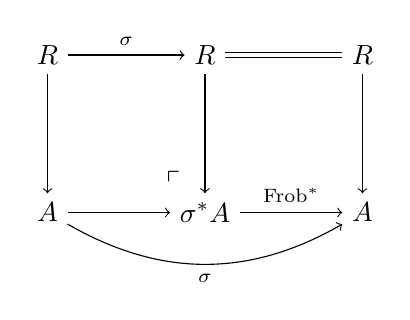
\begin{tikzpicture}[baseline=(current bounding box.center)]
         \node (LT) at (0, 2) {$R$}; 
         \node (MT) at (2, 2) {$R$}; 
         \node (RT) at (4, 2) {$R$}; 
         \node (LB) at (0, 0) {$A$}; 
         \node (MB) at (2, 0) {$\sigma^*A$}; 
         \node (RB) at (4, 0) {$A$}; 
         \node at (1.6, 0.4) {$\ulcorner$}; 
         \draw [->] (LT) -- node [above] {$\scriptstyle \sigma$} (MT); 
         \draw [double distance=1.3pt] (MT) -- (RT); 
         \draw [->] (LT) -- (LB); 
         \draw [->] (MT) -- (MB); 
         \draw [->] (RT) -- (RB); 
         \draw [->] (LB) -- (MB); 
         \draw [->] (MB) -- node [above] {$\scriptstyle \Frob^*$} (RB); 
         \draw [->] (LB) to [out = -30, in = -150] node [below] {$\scriptstyle \sigma$} (RB); 
 \end{tikzpicture}
\end{equation}
where $\sigma$ sends an element to its $p$'th power, and the left-hand 
square is a pushout of rings.  In particular, if $G$ is a formal group 
over $R$, there is an isogeny $\Frob \co G \to \sigma^*G$ of formal 
groups over $R$ defined by 
$\Frob^* \co \CO_{\sigma^*G} = \sigma^*\CO_G \to \CO_G$ which is the 
$R$-homomorphism 
\begin{equation*}
\begin{split}
 R \llbracket y \rrbracket \longrightarrow & ~ R \llbracket x \rrbracket \\
                    y ~ \mapsto \thinspace & ~ x^p.  
\end{split}
\end{equation*}

The Frobenius can be defined more generally for any complete local ring 
$R$ with maximal ideal $\fm$ (and $R$-algebras), by imposing the above 
commutative diagram on their mod-$p$ reductions.  This is indeed the 
generality we will be working with henceforth.  Our restricted first 
definition is simply for the clarity of exposition.  

Let $\pi \co R \to R/\fm$ be the natural quotient map.  A 
{\em deformation of $\BG$ to $R$} is a triple $(G,i,\A)$ consisting of a 
formal group $G$ over $R$, an inclusion $i \co k \to R/\fm$, and an 
isomorphism $\A \co \pi^*G \to i^*\BG$ of formal groups over $R/\fm$.  
Thus we have a diagram 
\begin{center}
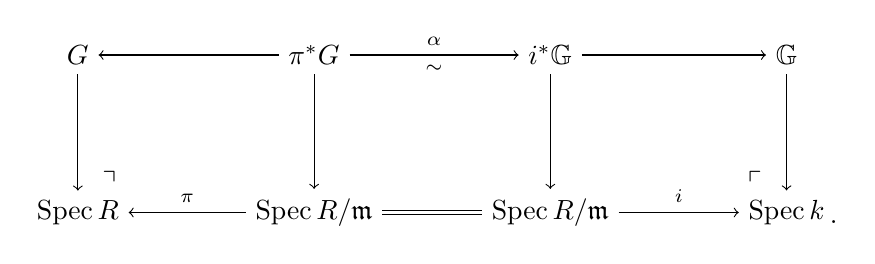
\begin{tikzpicture}
        \node (LT)  at (0, 2) {$G$}; 
        \node (MLT) at (3, 2) {$\pi^*G$}; 
        \node (MRT) at (6, 2) {$i^*\BG$}; 
        \node (RT)  at (9, 2) {$\BG$}; 
        \node (LB)  at (0, 0) {$\Spec R$}; 
        \node (MLB) at (3, 0) {$\Spec R/\fm$}; 
        \node (MRB) at (6, 0) {$\Spec R/\fm$}; 
        \node (RB)  at (9, 0) {$\Spec k$}; 
        \node at (9.6, -0.125) {.}; 
        \node at (0.4, 0.4) {$\urcorner$}; 
        \node at (8.6, 0.4) {$\ulcorner$}; 
        \draw [<-] (LT)  -- (MLT); 
        \draw [->] (MLT) -- node [above] {$\scriptstyle \A$} node [below] {$\scriptstyle \sim$} (MRT); 
        \draw [->] (MRT) -- (RT); 
        \draw [<-] (LB)  -- node [above] {$\scriptstyle \pi$} (MLB); 
        \draw [double distance=1.3pt] (MLB) -- (MRB); 
        \draw [->] (MRB) -- node [above] {$\scriptstyle i$} (RB); 
        \draw [->] (LT)  -- (LB); 
        \draw [->] (MLT) -- (MLB); 
        \draw [->] (MRT) -- (MRB); 
        \draw [->] (RT)  -- (RB); 
\end{tikzpicture}
\end{center}
We will simply write $\pi^*G$ as $G_0$, i.e., the special fiber of $G$ 
as a formal scheme over $R$.  Similarly, given an isogeny $\phi$ of 
formal groups, we write $\phi_0$ for the induced isogeny on the special 
fibers.  A {\em $\star$-isomorphism} $(G,i,\A) \to (G',i',\A')$ is an 
isomorphism $\phi \co G \to G'$ of formal groups over $R$ such that 
$i' = i$ and $\A' \circ \phi_0 = \A$.  

We define the {\em category of deformations of Frobenius over $R$} as 
follows.  

\begin{defn}
\label{def:DF}
 Let $\DF(R)$ be the category whose objects are deformations of $\BG$ to 
 $R$, and whose morphisms are isogenies which are {\em deformations of 
 Frobenius}, i.e., a morphism $(G,i,\A) \to (G',i',\A')$ is an isogeny 
 $\phi \co G \to G'$ such that $i' = \sigma^r \circ i$ and 
 $\A' \circ \phi_0 = \Frob^r \circ \A$ for some $r \geq 0$.  
\end{defn}

\begin{rmk}
\label{rmk:star}
 In the above definition, when $r = 0$, a morphism 
 $(G,i,\A) \to (G',i',\A')$ is precisely a $\star$-isomorphism.  
\end{rmk}

We then consider the category of sheaves of modules on 
$\DF \ce \{\DF(R)\}$.  

\begin{defn}
\label{def:mod}
 Define a category $\Mod_\DF$ as follows.  An object $\CF$ of this 
 category consists of the following data: 
 \begin{enumerate}[(i)]
  \item for each complete local ring $R$, a functor 
  \[
  \CF_R \co \DF(R)^\op \longrightarrow \Mod_R, 
  \]

  \item for each local homomorphism $f \co R \to S$, a natural 
  isomorphism 
  \[
  \CF_f \co f^*\CF_R \longrightarrow \CF_S ~f^* 
  \]
  where the first $f^*$ is the functor $\Mod_R \to \Mod_S$ of extending 
  scalars along $f$, and the second $f^* \co \DF(R)^\op \to \DF(S)^\op$ 
  is induced by $f$ ($\DF(-)$ is a functor), 
 \end{enumerate}
 together with natural isomorphisms 
 \[
  \CF_\id \cong \id \qquad \ad \qquad \CF_{gf} \cong 
  \CF_g(f^*) \circ g^*(\CF_f) 
 \]
 for all local homomorphisms $\id \co R \to R$, $f \co R \to S$, and 
 $g \co S \to T$.  

 A morphism $\eta \co \CF \to \CG$ in this category is a collection of 
 natural transformations 
 \[
  \eta_R \co \CF_R \longrightarrow \CG_R 
 \]
 together with natural isomorphisms 
 \[
  \CG_f \circ f^*(\eta_R) \cong \eta_S(f^*) \circ \CF_f.  
 \]
\end{defn}

\begin{ex}
 There is an object $\CO$ of $\Mod_\DF$ described as follows.  The 
 functor $\CO_R$ sends deformations to their base ring $R$, and sends 
 morphisms between deformations to the identity map of $R$.  The natural 
 isomorphism $\CO_f$ is determined by the isomorphism 
 \begin{equation*}
 \begin{split}
  R \tensor[]{\otimes}{_R^f} S \longrightarrow & ~ S \\
              r \otimes s ~ \mapsto \thinspace & ~ f(r) s.  
 \end{split}
 \end{equation*}
 The natural isomorphisms 
 \[
  \CO_\id \cong \id \qquad \ad \qquad \CO_{gf} \cong 
  \CO_g(f^*) \circ g^*(\CO_f) 
 \]
 are determined respectively by the isomorphisms 
 \begin{spacing}{.9}
  \[
   ~~ R \tensor[]{\otimes}{_R^\id} R \longrightarrow R \qquad \ad \qquad 
   R \tensor[]{\otimes}{_R^{gf}} T \longrightarrow 
   (R \tensor[]{\otimes}{_R^f} S) \tensor[]{\otimes}{_S^g} T.  
  \]
  \[
   \qquad r_1 \otimes r_2 ~ \mapsto ~ r_1 r_2 \qquad \qquad \qquad 
   ~ r \otimes t ~ \mapsto ~ (r \otimes 1) \otimes t \qquad \quad
  \]
 \end{spacing}
\end{ex}

\begin{rmk}
 The category $\Mod_\DF$ is symmetric monoidal with the tensor product 
 $\CF \otimes \CG$ given by 
 $(\CF \otimes \CG)_R(G) \ce \CF_R(G) \otimes_R \CG_R(G)$.  The unit 
 object is $\CO$ in the above example.  
\end{rmk}

\begin{thm}[{\cite[Pre-Theorem 16.4]{lpo}}]
 There is an equivalence of symmetric monoidal categories 
 \[
  \Mod_\CA \stackrel{\sim}{\longrightarrow} \Mod_\DF.  
 \]
\end{thm}

Next we consider $\Model_{\dl_{E_0}}$, the category of models for the 
theory $\dl_{E_0}$, on which $\CA$ acts.  By \cite[Proposition 7.6]{lpo}, 
there is a forgetful functor $\Model_{\dl_{E_0}} \to \Mod_\CA$ along 
which the coproduct of $\dl_{E_0}$-models and the tensor product of 
$\Mod_\CA$ agree.  

\begin{defn}
\label{def:alg}
 Define a category $\Alg_\DF$ as follows.  An object $\CB$ of this 
 category is a ring object in $\Mod_\DF$ satisfying the {\em Frobenius 
 congruence}, i.e., the diagram 
 \begin{center}
 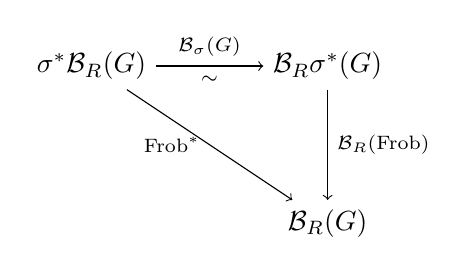
\begin{tikzpicture}
         \node (LT) at (0, 2) {$\sigma^*\CB_R(G)$}; 
         \node (RT) at (3, 2) {$\CB_R\sigma^*(G)$}; 
         \node (RB) at (3, 0) {$\CB_R(G)$}; 
         \draw [->] (LT) -- node [above] {$\scriptstyle \CB_\sigma(G)$} 
                            node [below] {$\scriptstyle \sim$} (RT); 
         \draw [->] (LT) -- node [left] {$\scriptstyle \Frob^*$} (RB); 
         \draw [->] (RT) -- node [right] {$\scriptstyle \CB_R(\Frob)$} (RB); 
 \end{tikzpicture}
 \end{center}
 commutes for all complete local rings $R$ and deformations $G$ of $\BG$ 
 to $R$.  

 Morphisms in this category are maps of ring objects.  

 An object $\CB$ is said to be {\em torsion free} if $\CB_R(G)$ is 
 $p$-torsion free for every $p$-torsion-free $R$ and every deformation 
 $G$ to $R$.  We denote by $\Alg_\DF^\tf$ the full subcategory of 
 $\Alg_\DF$ consisting of torsion-free objects.  
\end{defn}

\begin{rmk}
 We note as in \cite[11.18]{cong} that roughly speaking, the Frobenius 
 congruence is the requirement that $\CB$ carry the (relative) Frobenius 
 on formal groups to the (relative) Frobenius on algebras.  
\end{rmk}

Here is the key result bridging power operations and deformations of 
Frobenius (cf.~\cite[Theorem B]{cong}).  

\begin{thm}[{\cite[Pre-Theorem 16.5]{lpo}}]
\label{thm:bridge}
 There is a functor 
 \[
  \Model_{\dl_{E_0}} \longrightarrow \Alg_\DF.  
 \]
 It restricts to an equivalence 
 \[
  \Model_{\dl_{E_0}}^\tf \stackrel{\sim}{\longrightarrow} \Alg_\DF^\tf ~
 \]
 of full subcategories of torsion-free objects.  
\end{thm}


\subsection{Deformations of Frobenius are parametrized by subgroups}
\label{subsec:subgp}

Having identified the categories, we now analyze the essential data that 
are encoded in $\Mod_\DF$ and $\Alg_\DF^\tf$, by studying the structure 
of the category $\DF(R)$ of deformations of Frobenius.  This turns out 
to be parametrized by the finite flat subgroups of deformations of $\BG$ 
to $R$, as we explain below.  

Let $x$ be a coordinate on a formal group $G$ over $R$.  A 
{\em degree-$d$ subgroup $K$ of $G$} is an effective Cartier divisor on 
$G$ with $\CO_K = R \llbracket x \rrbracket / \big( f(x) \big)$ for some 
monic polynomial $f(x)$ of order $d$ such that 
\[
 f(x_1 +_G x_2) \in \big( f(x_1),~f(x_2) \big) \qquad \ad \qquad 
 f(x) \in (x), 
\]
i.e., the group law of $G$ restricts to $K$ and $K$ contains the 
identity.  In particular $K$ is finite and flat over $R$ (we will assume 
finiteness and flatness of subgroups even when we do not mention their 
degrees).  We have the {\em quotient group} $G/K$ which is again a 
formal group (see \cite[Section 5]{Str97}).  

One can show that the homomorphism $[d] \co G \to G$ restricts to zero 
on $K$ (see \cite[Section 1]{tateoort}), i.e., $f(x)$ divides $[d](x)$.  
Thus subgroups of a formal group over a $p$-local ring must have degree 
$p^r$ for some $r \geq 0$.  In particular, if $G$ is a formal group over 
a field $k$ of characteristic $p$, there is exactly one subgroup of 
degree $p^r$, given by $f(x) = x^{p^r}$, which is the kernel of the 
$r$-fold Frobenius isogeny $\Frob^r$.  

We have seen in Remark \ref{rmk:star} that in $\DF(R)$ the degree-1 
morphisms (when $r = 0$) are precisely the $\star$-isomorphisms of 
deformations.  In general, with morphisms corresponding to all 
$r \geq 0$, $\DF(R)$ is equivalent to the following category (see 
\cite[Proposition 16.9]{lpo}).  The objects of this category are 
$\star$-isomorphism classes of deformations $[G]$.  The morphisms are 
$\star$-isomorphism classes of pairs $[G>K]$: the source of $[G>K]$ is 
$[G]$, and the target of $[G>K]$ is $[G/K]$ where $G/K$ is a deformation 
of $\BG$ with $i_{G/K} = \sigma^r \circ i_G$ ($p^r$ being the degree of 
$K$).  Moreover, by the Lubin-Tate theorem (see 
\cite[Theorem 3.1]{lubintate} and \cite[Section 4.3]{Rnotes}), there is 
at most one $\star$-isomorphism between any two deformations.  If 
$[G/K] = [G']$, then 
\[
 [G'>K'] \circ [G>K] = [G>K''] 
\]
where $K''$ is the kernel of the composite 
\[
 G \to G/K \cong G' \to G'/K'.  
\]
Thus we see that deformations of Frobenius with source $(G,i,\A)$ 
correspond precisely to subgroups of $G$.  

\begin{ex}
\label{ex:K_p}
 Let $\BG$ be the multiplicative formal group over $\BF_p$ (of height 1).  
 For the multiplicative formal group $\HGm$ over a $p$-local ring $R$, 
 since the formal group law is defined by 
 \[
  1 + (x_1 +_\HGm x_2) \ce (1 + x_1)(1 + x_2), 
 \]
 we have 
 \[
  [p^r](x) = (1 + x)^{p^r} - 1, 
 \]
 which is a monic polynomial of order $p^r$.  Thus the only subgroups of 
 $\HGm$ are $\HGm [p^r]$ with 
 $\CO_{\HGm [p^r]} = \CO_\HGm \big/ \big( [p^r](x) \big)$.  Moreover, by 
 the Lubin-Tate theorem (see \cite[Theorem 3.1]{lubintate} and 
 \cite[Section 4.3]{Rnotes}), every object of $\DF(R)$ is 
 $\star$-isomorphic to $\HGm$, and the set of $\star$-isomorphism 
 classes of deformations of $\BG$ to $R$ is classified by the ring 
 $\CO_\univ \ce \BZ_p$.  In particular we can take the universal 
 deformation $G_\univ$ to be the multiplicative formal group over 
 $\BZ_p$.  Thus by functoriality, to describe an object $\CB$ of 
 $\Alg_\DF^\tf$, it is enough to give the following data: 
 \begin{enumerate}[(i)]
  \item a $p$-torsion free $\BZ_p$-algebra $B = \CB_{\BZ_p}(\HGm)$, 

  \item maps $\psi^{p^r} \co B \to B$ of $\BZ_p$-algebras (corresponding 
  to the isogenies $[p^r] \co \HGm \to \HGm$) such that 
  \begin{itemize}
   \item $\psi^1 = \id_B$ and 
   $\psi^{p^r} \circ \psi^{p^s} = \psi^{p^{r+s}}$, 

   \item $\psi^p(b) \equiv b^p \md pB$ (the Frobenius congruence).  
  \end{itemize}
 \end{enumerate}

 We note as in \cite[Example 1.3]{cong} that the above is a 
 ``$p$-typicalization'' of Wilkerson's theorem 
 \cite[Proposition 1.2]{wilkerson} which characterizes torsion-free 
 $\lambda$-rings in terms of the Adams operations satisfying the 
 Frobenius congruences at all primes.  More concretely, consider the 
 complex $K$-theory spectrum $KU$ (cf.~Example \ref{ex:KU}).  For 
 $B = \pi_0 A$, where $A$ is a $p$-complete $KU$-algebra (i.e., a 
 commutative $KU$-algebra such that $A \cong A_p^\wedge$), $\psi^p$ 
 recovers the $p$'th Adams operation studied by McClure (see 
 \cite[Chapters VIII and IX]{H_infty}).  
\end{ex}

In general, consider the functor $X_r$ which associates to a ring $R$ 
the set of $\star$-isomorphism classes of pairs $[G>K]$ with $K$ a 
degree-$p^r$ subgroup of $G$.  By \cite[Theorem 9.2]{Str98}, it is 
represented by the complete local ring 
\[
 \CO_{X_r} \ce E^0 B\Sigma_{p^r}/I 
\]
where 
\[
 I \ce \bigoplus_{0<i<p^r} {\rm image} 
 \big( E^0 B(\Sigma_i \times \Sigma_{p^r-i}) 
 \xrightarrow{\rm transfer} E^0 B\Sigma_{p^r} \big) 
\]
is the transfer ideal (cf.~\eqref{I}).  This can be viewed as a 
generalization of the Lubin-Tate theorem for $\CO_\univ = \CO_{X_0}$.  
Moreover there are two ring homomorphisms 
\[
 s^*, ~ t^* \co \CO_\univ \longrightarrow \CO_{X_r} 
\]
where $s^*$ represents the source map $[G>K] \mapsto [G]$, and $t^*$ 
represents the target map $[G>K] \mapsto [G/K]$.  Thus to describe an 
object $\CB$ of $\Alg_\DF^\tf$, it is enough to give the following data 
(subject to a set of formal properties): 
\begin{enumerate}[(i)]
 \item a $p$-torsion-free $\CO_\univ$-algebra 
 $B = \CB_{\CO_\univ}(G_\univ)$, 

 \item maps $\psi^{p^r} \co B \to B \otimes_{\CO_\univ}^{s^*} \CO_{X_r}$ 
 of $\CO_\univ$-algebras as the composites 
 \[
  B \to B \otimes_{\CO_\univ}^{t^*} \CO_{X_r} \stackrel{\CB_f}{\cong} 
  \CB_{\CO_{X_r}} (t^*G_\univ) \xrightarrow{\CB_{\CO_{X_r}} (\psi)} 
  \CB_{\CO_{X_r}} (s^*G_\univ) \stackrel{\CB_g}{\cong} 
  B \otimes_{\CO_\univ}^{s^*} \CO_{X_r} 
 \]
 where $f = t^*$ and $g = s^*$ are local homomorphisms, and 
 $\psi \co s^*G_\univ \to t^*G_\univ$ is the universal deformation of 
 $\Frob^r$ (see \cite[Section 13]{Str97}).  
\end{enumerate}
In particular, if we denote by $\phi^*$ the map 
\begin{equation}
\label{sigma}
 \CO_{X_1} \longrightarrow \CO_\univ/p\CO_\univ 
\end{equation}
which represents a universal Frobenius isogeny, the Frobenius congruence 
amounts to requiring that 
\begin{equation}
\label{frobcong}
 B \xrightarrow{\psi^p} B \otimes_{\CO_\univ}^{s^*} \CO_{X_1} 
 \xrightarrow{\id \otimes \phi^*} 
 B \otimes_{\CO_\univ} (\CO_\univ/p\CO_\univ) \cong B/pB 
\end{equation}
be the $p$'th-power map 
\[
 B \to B/pB \xrightarrow{\sigma} B/pB 
\]
which sends $b$ to $\overline{b}^p$.  

In Example \ref{ex:K_p}, $\CO_{X_r} \cong \CO_\univ$ for all $r$, that 
is, 
\[
 E^0 B\Sigma_{p^r}/I \cong E^0, 
\]
so that $s^* = t^* = \id$.  In fact this is true for any 
complex-oriented cohomology theory whose formal group is of height 1, as 
a height-1 formal group $\BG$ has a unique degree-$p^r$ subgroup 
$\BG [p^r]$ (classified by $\CO_{X_r}$) for each $r$.  Thus by Theorem 
\ref{thm:bridge}, the power operation structure on a $K(1)$-local Morava 
$E$-theory at the prime $p$ is simple: the operation 
$\psi^p \co E^0 \to E^0$, which is a lift of the Frobenius map, 
determines the other $\psi^{p^r}$ with $r>1$ by iterated composition.  
In particular, when $E_*$ is $p$-torsion free, $\psi^p$ determines 
{\em all} the power operations so that $E_*$ has the structure of a 
{\em free Frobenius algebra with one generator} on which $\psi^p$ acts 
(cf.~\cite[Section 4]{hopkins}).  

Here is an example for $\BG$ of height 2 studied by Rezk \cite{h2p2}.  

\begin{ex}
\label{ex:h2p2b}
 Consider the elliptic curve\footnote{See, for example, Section 
 \ref{sec:ec} for some of the basics about elliptic curves.  } 
 $C_0 \subset \BP_{\BF_2}^2$ defined by 
 \[
  Y^2 Z + Y Z^2 = X^3, 
 \]
 which is supersingular so that its formal group $\HC_0$ is of height 2.  
 It has a universal deformation $C$ over the Lubin-Tate ring 
 $\BW(\BF_2) \llbracket u_1 \rrbracket \cong 
 \BZ_2 \llbracket a \rrbracket$ given by 
 \[
  Y^2 Z + a X Y Z + Y Z^2 = X^3 
 \]
 where $a$ is the Hasse invariant (cf.~\cite[Proposition 3.2]{tmf3} and 
 \cite[2.2.10]{KM}).  Setting $a=0$ we recover the supersingular 
 elliptic curve $C_0$.  Let $E$ be the Morava $E$-theory spectrum 
 associated to $\HC_0/\BF_2$, so that 
 \[
  E_* \cong \BZ_2 \llbracket a \rrbracket [u^{\pm 1}] 
 \]
 with $|u| = 2$.  

 By studying degree-2 subgroups of $C$, i.e., subgroups generated by 
 2-torsion points on $C$, Rezk identifies that 
 \[
  \CO_{X_1} \cong \BZ_2 \llbracket a, d \rrbracket / (d^3 - a d - 2), 
 \]
 i.e., in the affine coordinate chart $\{u = X/Y, v = Z/Y\}$, degree-2 
 subgroups are generated by points $Q$ of the form 
 $\big( u(Q), v(Q) \big) = (d, -d^3)$ with $d^3 - a d - 2 = 0$.  Thus 
 there is a power operation 
 \[
  \psi^2 \co E^0 \longrightarrow E^0 \llbracket d \rrbracket / 
  (d^3 - a d - 2).  
 \]
 Moreover, by studying the universal isogeny with source $C$ and kernel 
 the degree-2 subgroup generated by $Q$ (cf.~\cite[Theorem 1.4]{lubin}), 
 Rezk computes that 
 \[
  t^* (a) = \psi^2 (a) = a^2 + 3 d - a d^2.  
 \]
 He also gives formulas for individual power operations $Q_0$, $Q_1$, 
 and $Q_2$ which express 
 \[
  \psi^2 (x) = Q_0(x) + Q_1(x) d + Q_2(x) d^2 
 \]
 (see Example \ref{ex:h2p2a}).  In particular the Frobenius congruence 
 takes the form 
 \[
  Q_0(x) \equiv x^2 \md 2.  
 \]
\end{ex}


\section{Subgroups of elliptic curves}
\label{sec:ec}

We have seen in Section \ref{subsec:E} that there is a connection 
between complex-oriented cohomology theories and one-dimensional 
commutative formal groups, via Chern classes of line bundles, which 
gives rise to the chromatic filtration.  In particular the formal groups 
for ordinary cohomology and complex $K$-theory turn out to be the 
additive formal group $\HGa$ and the multiplicative formal group $\HGm$ 
respectively (see \cite[Example 2.14, and Sections 1 and 7]{coctalos}, 
and cf.~Example \ref{ex:K_p}).  These are formal completions of 
one-dimensional group schemes.  Apart from the additive and 
multiplicative groups, the only other possibility of a one-dimensional 
group scheme over an algebraically closed field is an elliptic curve 
(see \cite[IV.1.6]{AECII}, and cf.~\cite[Section 12]{tafoverview}).  

Throughout this section we will use a specific example (starting as 
Example \ref{ex:C}) to illustrate the theory related to subgroups of 
elliptic curves.  Via the bridge discussed in Section \ref{sec:fg} 
(particularly Theorem \ref{thm:bridge}), the calculations we do with 
this example will be used for computing power operations in Section 
\ref{sec:p3}.  


\subsection{The group structure}
\label{subsec:gp}

Let $S$ be a scheme.  By a {\em smooth curve $E/S$}, we mean a smooth 
morphism 
\[
 \pi \co E \longrightarrow S 
\]
of relative dimension one which is separated and of finite presentation.  
An {\em elliptic curve $E/S$} is a proper smooth curve with 
geometrically connected fibers all of genus one together with a section 
$O \in E(S)$.  There is a unique structure of commutative $S$-group 
scheme on $E/S$ for which $O$ is the identity (see 
\cite[2.1.2 and 2.5.1]{KM}), and thus the formal completion $\HE$ of $E$ 
at $O$ is a one-dimensional commutative formal group.  Visibly (a fiber 
of) such a (relative) curve, with the group law on it, is depicted on 
the front cover of \cite[second ed.]{AEC}; the interested reader might 
also seek out Bryan Birch's birthday card.  More concretely, we can 
describe an elliptic curve and do calculations with its group law using 
a {\em Weierstrass equation}.  

\subsubsection*{Weierstrass equations}

Locally on some affine open subset $\Spec R \subset S$, any elliptic 
curve $E/S$ has a presentation as the locus in $\BP_R^2$ of a 
Weierstrass equation 
\begin{equation}
\label{XYZ}
 Y^2 Z + a_1 X Y Z + a_3 Y Z^2 = X^3 + a_2 X^2 Z + a_4 X Z^2 + a_6 Z^3 
\end{equation}
where $a_i \in R$, with $O = [0,1,0]$.  In the affine coordinate chart 
$\{x = X/Z, y = Y/Z\}$, this becomes 
\begin{equation}
\label{xy}
 y^2 + a_1 x y + a_3 y = x^3 + a_2 x^2 + a_4 x + a_6 
\end{equation}
with $O$ at the infinity.  Associated to $E/R$ given as above, we have 
the following quantities (see Caution \ref{cau} below): 
\begin{equation}
\label{quantities}
\begin{split}
 b_2 \ce & ~ a_1^2 + 4 a_2, \\
 b_4 \ce & ~ 2 a_4 + a_1 a_3, \\
 b_6 \ce & ~ a_3^2 + 4 a_6, \\
 b_8 \ce & ~ a_1^2 a_6 + 4 a_2 a_6 - a_1 a_3 a_4 + a_2 a_3^2 - a_4^2, \\
 \Delta \ce & ~ -b_2^2 b_8 - 8 b_4^3 - 27 b_6^2 + 9 b_2 b_4 b_6, \\
 \omega \ce & ~ -\frac{dx}{2 y + a_1 x + a_3} = \frac{dy}{a_1 y - 3 x^2 - 2 a_2 x - a_4}.  
\end{split}
\end{equation}
Here $\Delta$ is invertible in $R$ so that $E$ is smooth.  The one-form 
$\omega$ is nowhere vanishing, and is invariant under translation by the 
group law on $E$.  Locally it is an $R$-basis of the invertible sheaf 
\[
 \om \ce \pi_* \Omega_{E/S}, 
\]
the pushforward along the structure morphism $\pi \co E \to S$ of the 
relative cotangent sheaf $\Omega_{E/S}$, on which the multiplicative 
group $\Gm \ce \Spec R[\lambda^{\pm1}]$ acts by 
\begin{equation}
\label{action}
 \omega \longmapsto \lambda \omega.  
\end{equation}
This action lifts to one on $E/R$ with 
\[
 (x,y) \mapsto (\lambda^{-2} x,\lambda^{-3} y) \qquad \ad \qquad 
 a_i \mapsto \lambda^{-i} a_i \text{~ for all ~} i, 
\]
and we have a compatible grading that 
\[
 |x| = 2, \qquad |y| = 3, \qquad \ad \qquad |a_i| = i.  \qquad \qquad 
 \quad
\]
Keeping track of this grading is helpful in calculations with elliptic 
curves.  The only change of variables fixing $O$ and preserving the form 
of \eqref{xy} is 
\[
 x = u^2 x' + r \qquad \ad \qquad y = u^3 y' + u^2 s x' + t 
\]
where $r$, $s$, $t \in R$ and $u \in R^\times$.  

When we study the formal completion of $E$ at $O$, it is convenient to 
work in the affine coordinate chart $\{u = X/Y, v = Z/Y\}$ so that 
$O = (0,0)$.  In $uv$-coordinates, the Weierstrass equation \eqref{XYZ} 
becomes 
\[
 v + a_1 u v + a_3 v^2 = u^3 + a_2 u^2 v + a_4 u v^2 + a_6 v^3, 
\]
and we have 
\[
 u = \frac{x}{y}, \quad v = \frac{1}{y}, \qquad {\rm or} \qquad 
 x = \frac{u}{v}, \quad y = \frac{1}{v}, 
\]
with 
\[
 ~~ |u| = -1 \qquad \ad \qquad |v| = -3.  
\]
In particular, the formal group $\HE$ has $u$ as a coordinate which is 
{\em adapted to $\omega$} in the sense that 
\begin{equation}
\label{adapted}
 \omega|_{\HE} = \big( 1 + (\text{higher-order terms}) \big) du 
\end{equation}
(cf.~\cite[IV.1]{AEC}).  

\begin{cau}
\label{cau}
 In some sources (e.g., \cite[IV.1]{AEC} and \cite[Section 9]{pearson}) 
 the formulas for $u$ and $v$, as well as that for $\omega$, differ from 
 ours by a minus sign.  
\end{cau}

\subsubsection*{Rigidity and duality}

As a geometric manifestation of the group structure, the following 
rigidity property of elliptic curves is important to our later 
discussion (see Remark \ref{rmk:rig} and the proof of Proposition 
\ref{prop:frob^2}).  

\begin{thm}[{\cite[2.4.2]{KM}}]
 Let $S$ be a scheme, $E_1$ and $E_2$ two elliptic curves over $S$, and 
 $\phi \co E_1 \to E_2$ an $S$-homomorphism.  Then Zariski-locally on 
 $S$, either $\phi = 0$ or $\phi$ is an {\em isogeny}, i.e., $\phi$ is 
 finite locally free.  
\end{thm}

\begin{cor}
\label{cor:rig}
 Hypotheses and notations as in the above theorem, suppose $S$ is 
 connected.  If $\phi_x \co (E_1)_x \to (E_2)_x$ is zero for some 
 $x \in S$ where $(-)_x$ denotes the fiber over $x$ along the structure 
 morphism, then $\phi = 0$.  
\end{cor}

\begin{rmk}
\label{rmk:rig}
 Some of the formulas involved in our later calculations with elliptic 
 curves are in fact valid only fiber by fiber over the base scheme (for 
 example, the group law algorithm in Example \ref{ex:C}, the division 
 polynomial $\psi_3$ in the proof of Proposition \ref{prop:tors}, 
 V\'elu's formulas in Example \ref{ex:velu}, and the changes of 
 variables in Example \ref{ex:velu} and in the proof of Proposition 
 \ref{prop:C}).  As our base scheme is connected, the statements for 
 elliptic curves over the entire base scheme follow by rigidity.  We 
 will write those formulas formally to streamline the exposition.  
\end{rmk}

As a consequence of rigidity (essentially of the group structure), every 
isogeny $\phi \co E_1 \to E_2$ of degree $d$ over a connected base 
scheme $S$ has a {\em dual isogeny} $\Hphi \co E_2 \to E_1$ of the same 
degree such that $\Hphi \circ \phi = [d]$ (see \cite[2.6.1]{KM}).  In 
particular, if $\phi \co E \to E$ is an endomorphism, then in the 
endomorphism ring of $E$, $\phi$ is a root of the polynomial 
\begin{equation}
\label{poly}
 X^2 - \tr(\phi) \cdot X + d = 0 
\end{equation}
with $\tr(\phi) \ce \phi + \Hphi$ an integer satisfying 
\[
 \big( \tr(\phi) \big)^2 - 4 d \leq 0 
\]
(see \cite[2.6.2.2 and 2.6.3]{KM}).  

\subsubsection*{Calculations}

\begin{ex}
\label{ex:C}
 Consider the curve in $\BP^2$ given by the affine equation 
 \begin{equation}
 \label{Cxy}
  C \co y^2 + a x y + a b y = x^3 + b x^2 
 \end{equation}
 over $\BZ [a, b]$.  Not knowing if it is an elliptic curve, we compute 
 formally according to \eqref{quantities} that 
 \begin{equation*}
 \begin{split}
     b_2 = & ~ a^2 + 4 b, \quad b_4 = a^2 b, \quad b_6 = a^2 b^2, \quad b_8 = a^2 b^3, \\
  \Delta = & ~ a^2 b^4 (a^2 - 16 b), \\
  \omega = & ~ -dx / (2 y + a x + a b) = dy / (a y - 3 x^2 - 2 b x).  
 \end{split}
 \end{equation*}
 Thus $C$ is an elliptic curve over the graded ring 
 \[
  \s \ce \BZ [1/4] [a, b, \Delta^{-1}] 
 \]
 where $|a| = 1$ and $|b| = 2$.  The invertibility of 4 in $\s$ allows 
 us to characterize 4-torsion points on $C$ as below.  

 Let $P_0 \ce (0,0)$.  Since from the formula for $\omega$ we have 
 \[
  \frac{dy}{dx} = \frac{3 x^2 + 2 b x - a y}{2 y + a x + a b}, 
 \]
 the tangent line of $C$ at $P_0$ is $y = 0$.  By the group law as 
 geometrically depicted, $2P_0$ is then the other point where $y = 0$ 
 and $C$ intersect, namely, $(-b,0)$.  We compute that the tangent line 
 at $2P_0$ is $x = -b$, and thus $4P_0$ is the identity $O$ at the 
 infinity.  Conversely, as 4 is invertible in $\s$, any 4-torsion point 
 $P$ has the above property: the tangent line at $P$ passes through a 
 point $P'$ such that the tangent line at $P'$ is vertical.  

 In $uv$-coordinates, the equation \eqref{Cxy} of $C$ becomes 
 \begin{equation}
 \label{Cuv}
  v + a u v + a b v^2 = u^3 + b u^2 v.  
 \end{equation}
 In terms of an algorithm, the group law on $C$ satisfies: 
 \begin{itemize}
  \item given $P(u,v)$, the coordinates of $-P$ are 
  \[
   \left( -\frac{v}{u (u + b v)},-\frac{v^2}{u^2 (u + b v)} \right); 
  \]

  \item given $P_1(u_1,v_1)$ and $P_2(u_2,v_2)$, the coordinates of 
  $-(P_1 + P_2)$ are 
  \[
   u_3 \ce a k - \frac{b m}{1 + b k} - u_1 - u_2 \qquad \ad \qquad 
   v_3 \ce k u_3 + m 
  \]
  where 
  \[
   k = \frac{v_1 - v_2}{u_1 - u_2} \qquad \ad \qquad 
   m = \frac{u_1 v_2 - u_2 v_1}{u_1 - u_2}.  
  \]
 \end{itemize}
 Given $P(u,v)$ and $Q(d,e)$, with the above notations and formulas, we 
 then have: 
 \begin{itemize}
  \item set 
  \[
   (u_1,v_1) = \left( -\frac{v}{u (u + b v)}, 
   -\frac{v^2}{u^2 (u + b v)} \right) \qquad \ad \qquad (u_2,v_2) = (d,e) 
  \]
  so that 
  \[
   P - Q = (u_3,v_3); 
  \]

  \item set 
  \[
   (u_1,v_1) = (u,v) \qquad \ad \qquad (u_2,v_2) = (d,e) 
  \]
  so that 
  \[
   P + Q = \left( -\frac{v_3}{u_3 (u_3 + b v_3)}, 
   -\frac{v_3^2}{u_3^2 (u_3 + b v_3)} \right).  
  \]
 \end{itemize}
\end{ex}


\subsection{Torsion subgroups}
\label{subsec:tors}

In Example \ref{ex:C} we looked at a 4-torsion point $P_0$ on an 
elliptic curve $C$ over a ring $\s$ where 4 is invertible.  Here is the 
general structure of the subgroup of $m$-torsion points on an elliptic 
curve (cf.~\cite[2.3.2 and 12.2.6]{KM}).  

\begin{thm}[{\cite[2.3.1]{KM}}]
\label{thm:tors}
 Let $S$ be a scheme, $E/S$ an elliptic curve, and $m \geq 1$ an integer.  
 Then the {\em multiplication-by-$m$} homomorphism 
 \[
  [m] \co E \longrightarrow E 
 \]
 over $S$ is finite locally free of rank $m^2$.  If $m$ is invertible on 
 $S$, its kernel $E[m]$ is finite \'etale over $S$, locally for the 
 \'etale topology on $S$ isomorphic to 
 $\underline{\BZ/m} \times \underline{\BZ/m}$.  
\end{thm}

To compute an $m$-torsion point on an elliptic curve $E$ over a field in 
the Weierstrass equation \eqref{xy}, with the quantities $b_i$ as in 
\eqref{quantities}, we introduce {\em division polynomials} 
(cf.~\cite[Exercise 3.7]{AEC} and \cite[13(9.2-4)]{husemoller}).  

\begin{defn}
\label{def:division}
 Define polynomials $\psi_m \in \BZ[a_1,\ldots,a_4,a_6,x,y]$, $m \geq 0$, 
 using the initial values 
 \begin{equation*}
 \begin{split}
  \psi_0 = & ~ 0, \\
  \psi_1 = & ~ 1, \\
  \psi_2 = & ~ 2 y + a_1 x + a_3, \\
  \psi_3 = & ~ 3 x^4 + b_2 x^3 + 3 b_4 x^2 + 3 b_6 x + b_8, \\
  \psi_4 = & ~ \psi_2 \big( 2 x^6 + b_2 x^5 + 5 b_4 x^4 + 10 b_6 x^3 + 10 b_8 x^2 + (b_2 b_8 - b_4 b_6) x + b_4 b_8 - b_6^2 \big), 
 \end{split}
 \end{equation*}
 and then inductively by the formulas 
 \begin{equation*}
 \begin{split}
       \psi_{2m+1} = & ~ \psi_{m+2} \psi_m^3 - \psi_{m-1} \psi_{m+1}^3, \qquad \qquad \qquad ~\thinspace {\rm for} ~ m \geq 2, \\
  \psi_2 \psi_{2m} = & ~ \psi_{m-1}^2 \psi_m \psi_{m+2} - \psi_{m-2} \psi_m \psi_{m+1}^2, \qquad \quad {\rm for} ~ m \geq 3.  
 \end{split}
 \end{equation*}
 Define polynomials $\phi_m$, $\omega_m \in \BZ[a_1,\ldots,a_4,a_6,x,y]$, 
 $m \geq 2$, by 
 \begin{equation*}
 \begin{split}
             \phi_m = & ~ x \psi_m^2 - \psi_{m+1} \psi_{m-1}, \\
  2 \psi_2 \omega_m = & ~ \psi_{m-1}^2 \psi_{m+2} - \psi_{m-2} \psi_{m+1}^2.  \qquad \qquad \qquad \qquad \quad ~~
 \end{split}
 \end{equation*}
\end{defn}

By \cite[Exercise 3.7d and f]{AEC}, for $m \geq 2$ and any point 
$P(x,y)$ on $E$, we have 
\begin{equation}
\label{[m]}
 [m] (x,y) = \left( \frac{\phi_m}{\psi_m^2}, 
 \frac{\omega_m}{\psi_m^3} \right), 
\end{equation}
and $\psi_m$ vanishes at precisely the nonzero $m$-torsion points.  

\subsubsection*{Calculations}

As a continuation of Example \ref{ex:C}, we compute the nonzero 
3-torsion points on the elliptic curve $C$.  

\begin{prop}
\label{prop:tors}
 On the elliptic curve $C$ over $\s$, the $uv$-coordinates $(d,e)$ of 
 any nonzero 3-torsion point satisfy the identities 
 \begin{equation}
 \label{f}
  f(d) = 0 
 \end{equation}
 and 
 \begin{equation}
 \label{g}
  e = g(d) 
 \end{equation}
 where $f$, $g \in \s [u]$ are given by 
 \begin{equation*}
 \begin{split}
  f(u) = & ~ b^4 u^8 + 3 a b^3 u^7 + 3 a^2 b^2 u^6 + (a^3 b + 7 a b^2) u^5 + (6 a^2 b - 6 b^2) u^4 + 9 a b u^3 \\
         & + (-a^2 + 8 b) u^2 - 3 a u - 3, \\
  g(u) = & -\frac{1}{a (a^2 - 16 b)} \big( a b^3 u^7 + (3 a^2 b^2 - 2 b^3) u^6 + (3 a^3 b -6 a b^2) u^5 + (a^4 + a^2 b \\
         & + 2 b^2) u^4 + (4 a^3 - 15 a b) u^3 + 18 b u^2 - 12 a u - 18 \big).  
 \end{split}
 \end{equation*}
\end{prop}
\begin{proof}
 \footnote{See Appendix \ref{apx:tors} for explicit formulas for the 
 polynomials $\Tf$, $Q_1$, $R_1$, $Q_2$, $R_2$, $K$, $L$, $M$, and $N$ 
 that appear in the proof.  }
 Given the elliptic curve $C$ with equation \eqref{Cxy}, a nonzero point 
 $Q$ is 3-torsion if and only if the polynomial 
 \begin{equation}
 \label{psi_3}
  \psi_3 (x) = 3 x^4 + (a^2 + 4 b) x^3 + 3 a^2 b x^2 + 3 a^2 b^2 x 
  + a^2 b^3 
 \end{equation}
 in Definition \ref{def:division} vanishes at $Q$.  Substituting 
 $x = u/v$ and clearing the denominators, we get a polynomial 
 \[
  \Tp_3(u,v) \ce 3 u^4 + (a^2 + 4 b) u^3 v + 3 a^2 b u^2 v^2 
  + 3 a^2 b^2 u v^3 + a^2 b^3 v^4.  
 \]
 As $Q = (d,e)$ in $uv$-coordinates, we then have 
 \begin{equation}
 \label{Tp}
  \Tp_3(d,e) = 0.  
 \end{equation}

 To get the polynomial $f$, we take $v$ as variable and rewrite 
 \eqref{Cuv} as a quadratic equation 
 \begin{equation}
 \label{quadratic}
  a b v^2 + (-b u^2 + a u + 1) v - u^3 = 0, 
 \end{equation}
 where the leading coefficient $a b$ is invertible in 
 $\s = \BZ [1/4] [a, b, \Delta^{-1}]$ as 
 $\Delta = a^2 b^4 (a^2 - 16 b)$.  Define 
 \begin{equation}
 \label{Tfdef}
  \Tf(u) \ce \Tp_3(u,v) \Tp_3(u,\bar{v}) 
 \end{equation}
 where $v$ and $\bar{v}$ are formally the conjugate roots of 
 \eqref{quadratic} so that we compute $\Tf$ in terms of $u$ by 
 substituting 
 \[
  v + \bar{v} = \frac{b u^2 - a u - 1}{a b} \qquad \ad \qquad 
  v \bar{v} = -\frac{u^3}{a b}.  
 \]
 We then factor $\Tf$ over $\s$ as 
 \begin{equation}
 \label{Tffactor}
  \Tf(u) = -\frac{u^4 f(u)}{a^2 b} 
 \end{equation}
 with $f$ the stated polynomial of order 8.  We check that $f$ is 
 irreducible by applying Eisenstein's criterion to the homogeneous prime 
 ideal $(3,H)$ of $\s$.  

 We have $\Tf(d) = 0$ by \eqref{Tfdef} and \eqref{Tp}.  To see 
 $f(d) = 0$, consider the closed subscheme $D \subset C[3]$ of nonzero 
 3-torsion points.  By Theorem \ref{thm:tors} it is finite locally free 
 of rank 8 over $\s$.  By the Cayley-Hamilton theorem, as a global 
 section of $D$, $u$ locally satisfies a homogeneous monic equation of 
 order 8, and this equation locally defines the rank-8 scheme $D$.  
 Since $D$ is affine, it is then globally defined by such an equation.  
 In view of $\Tf(d) = 0$ and \eqref{Tffactor}, we determine this 
 equation, and (up to a unit in $\s$) get the first stated identity 
 \eqref{f}.  

 To get the polynomial $g$, we note that both the quartic polynomial 
 \[
  A(v) \ce \Tp_3(d,v) 
 \]
 and the quadratic polynomial 
 \[
  B(v) \ce a b v^2 + (-b d^2 + a d + 1) v - d^3 
 \]
 defined from \eqref{quadratic} vanish at $e$, and thus so does their 
 greatest common divisor (gcd).  Applying the Euclidean algorithm (see 
 Appendix \ref{apx:tors} for explicit expressions), we have 
 \begin{equation*}
 \begin{split}
  A(v) = & ~ Q_1(v) B(v) + R_1(v), \\
  B(v) = & ~ Q_2(v) R_1(v) + R_2, 
 \end{split}
 \end{equation*}
 where 
 \[
  R_1(v) = K(d) v + L(d) 
 \]
 for some polynomials $K$ and $L$, and $R_2 = 0$ in view of \eqref{f}.  
 Thus $R_1(v)$ is the gcd of $A(v)$ and $B(v)$, and hence 
 \[
  K(d) e + L(d) = R_1(e) = 0.  
 \]
 To write $e$ in terms of $d$ from the above identity, we apply the 
 Euclidean algorithm to $f$ and $K$.  Their gcd turns out to be 1, and 
 thus there are polynomials $M$ and $N$ with 
 \[
  M(u) f(u) + N(u) K(u) = 1.  
 \]
 By \eqref{f} we then have $N(d) K(d) = 1$, and thus 
 \[
  e = -N(d) L(d) = g(d) 
 \]
 where $g$ is as stated.  
\end{proof}


\subsection{The formal group}
\label{subsec:fg}

\subsubsection*{The $p$-divisible group and deformation theory}

In Section \ref{subsec:tors} we looked at the torsion subgroups $E[m]$ 
of an elliptic curve $E/S$.  In particular, for a prime $p$, consider 
\[
 E[p^\infty] \ce \bigcup_{n \geq 0} E[p^n].  
\]
It is a {\em $p$-divisible group of height 2} in the sense of 
\cite[Section 2.1]{tate}.  The following theorem of Serre and Tate 
states that $p$-adically the deformation theory of an elliptic curve is 
equivalent to the deformation theory of its $p$-divisible group.  

\begin{thm}[Serre-Tate, see {\cite[2.9.1]{KM}}]
\label{thm:serretate}
 Let $R$ be a ring, $I$ an ideal of $R$, and $p$ a prime number.  
 Suppose that the ideal $(I,p)$ is nilpotent.  Denote by $R_0$ the ring 
 $R/I$.  Consider the following two categories: 
 \begin{equation*}
 \begin{split}
  \CA: ~ & ~ \text{objects are elliptic curves $E/R$, morphisms are $R$-homomorphisms; }\\
  \CC: ~ & ~ \text{objects are triples $(E_0/R_0, \BG/R, i)$ with }\\
         & ~ \quad \text{$E_0/R_0$ an elliptic curve, }\\
         & ~ \quad \text{$\BG/R$ a $p$-divisible group, and }\\
         & ~ \quad \text{$i$ an $R_0$-isomorphism $E_0[p^\infty] \xrightarrow{\sim} \BG \otimes_R R_0$ of $p$-divisible groups, }\\
         & ~ \text{morphisms are pairs $(\phi_0, \phi)$ with }\\
         & ~ \quad \text{$\phi_0$ an $R_0$-homomorphism of elliptic curves, }\\
         & ~ \quad \text{$\phi$ an $R$-homomorphism of $p$-divisible groups, such that }\\
         & ~ \quad \text{$\phi_0$ and $\phi \otimes_R R_0$ agree (via $i$) on the $p$-divisible groups over $R_0$.  }
 \end{split}
 \end{equation*}
 Then the functor $\CA \to \CC$ defined on objects by 
 \[
  E/R \longmapsto \big( (E \otimes_R R_0) / R_0, E[p^\infty], \id \big) 
 \]
 is an equivalence of categories.  
\end{thm}

We will come back to this theorem when we discuss a universal 
deformation of a specific elliptic curve in Example \ref{ex:E}.  

Associated to any $p$-divisible group $\BG$ over a complete noetherian 
local ring $R$ there is an exact sequence 
\begin{equation}
\label{ses}
 0 \to \BG^0 \to \BG \to \BG^{\rm et} \to 0 
\end{equation}
of $p$-divisible groups over $R$, natural in $\BG$, where $\BG^0$ is 
formal and $\BG^{\rm et}$ is \'etale, and the sum of their heights 
equals the height of $\BG$ (see \cite[Section 2.2]{tate}).  In 
particular, when $\BG = E[p^\infty]$ with $E$ an elliptic curve over a 
field $k$ of characteristic $p$, $\BG^0$ coincides with $\HE$, and the 
height of $\BG^0$ as a $p$-divisible group agrees with the {\em height} 
of $\HE$ as a formal group (the latter notion we will recall below).  
With motivation from algebraic topology, we are particularly interested 
in the case when $\HE$ is of height 2, so that $E[p^\infty]$ is all 
formal, i.e., there is no \'etale component in \eqref{ses}.  

Let $\G$ be a formal group over a perfect field $k$ of characteristic 
$p$.  Recall that the {\em height of $\G$}, denoted by $\HT(\G)$, is 
defined to be the largest integer $n$ such that 
\[
 [p](u) = f(u^{p^n}) 
\]
for some $f(u) \in k \llbracket u \rrbracket = \CO_\G$ (if $[p] = 0$, we 
set $\HT(\G) \ce \infty$).  In particular, for an elliptic curve $E/k$, 
$\HT(\HE)$ is either 1 or 2 (see \cite[IV.7.5]{AEC}), and 
correspondingly the elliptic curve is said to be {\em ordinary} or 
{\em supersingular}.  This dichotomy of elliptic curves has a geometric 
characterization as below (cf.~\cite[12.4.1]{KM}).  

\subsubsection*{The Hasse invariant and supersingularity}

Let $E/S/\BF_p$ be an elliptic curve over an $\BF_p$-scheme.  Recall 
that the absolute Frobenius of $E$, affine-locally given by the ring 
homomorphism $x \mapsto x^p$, has a canonical factorization through the 
relative Frobenius $F$ (cf.~\eqref{relFrob2} and \eqref{relFrob1}): 
\begin{center}
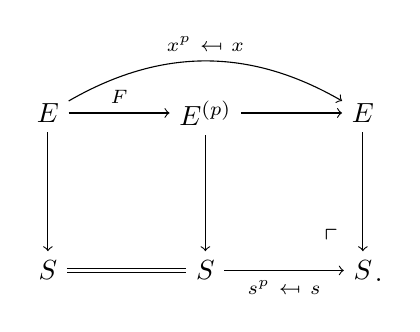
\begin{tikzpicture}
        \node (LT) at (0, 2) {$E$}; 
        \node (MT) at (2, 2) {$E^{(p)}$}; 
        \node (RT) at (4, 2) {$E$}; 
        \node (LB) at (0, 0) {$S$}; 
        \node (MB) at (2, 0) {$S$}; 
        \node (RB) at (4, 0) {$S$}; 
        \node at (4.2, -0.125) {.}; 
        \node at (3.6, 0.4) {$\ulcorner$}; 
        \draw [->] (LT) -- node [above] {$\scriptstyle F$} (MT); 
        \draw [double distance=1.3pt] (LB) -- (MB); 
        \draw [->] (LT) -- (LB); 
        \draw [->] (MT) -- (MB); 
        \draw [->] (RT) -- (RB); 
        \draw [->] (MT) -- (RT); 
        \draw [->] (MB) -- node [below] {$\scriptstyle s^p ~ \mapsfrom ~ s$} (RB); 
        \draw [->] (LT) to [out = 30, in = 150] node [above] {$\scriptstyle x^p ~ \mapsfrom ~ x$} (RT); 
\end{tikzpicture}
\end{center}
Denote by $V \co E^{(p)} \to E$ the Verschiebung dual to $F$ so that 
$V \circ F = [p]$.  Define {\em the Hasse invariant} $H$ as a modular 
form of weight $p-1$ given by the tangent map of $V$: 
\begin{equation*}
\begin{split}
 V_* \in & ~ \Hom_S \big( \CLie(E^{(p)}/S), \CLie(E/S) \big) \\
       = & ~ \Hom_S \big( \CLie(E/S)^{\otimes p}, \CLie(E/S) \big) \\
       = & ~ \Hom_S \big( \CO_S, (\om)^{\otimes (p-1)} \big) \\
       = & ~ H^0 \big( S, (\om)^{\otimes (p-1)} \big) 
\end{split}
\end{equation*}
where the $\CO_S$-module $\CLie(E/S) \cong (\om)^\vee$ is the 
pushforward to $S$ of the relative tangent sheaf on $E/S$ along the 
structure morphism.  

Locally on $\Spec R \subset S$ pick an $R$-basis $\omega$ as we did in 
Section \ref{subsec:gp}.  In terms of the bases of $\CLie(E^{(p)}/S)$ 
and $\CLie(E/S)$ dual to $\omega$, the Hasse invariant $H(E,\omega)$ is 
then an element in $R$.  In particular, for the formal group $\HE$ with 
a coordinate $u$ adapted to $\omega$ (see \eqref{adapted}), since 
\[
 [p](u) = V \circ F (u) = V(u^p), 
\]
we see that $H(E,\omega)$ is the coefficient of $u^p$ in $[p](u)$.  Thus 
$\HE$ is of height 2 if and only if $H(E,\omega) = 0$.  The following 
theorem of Igusa gives a precise description of the vanishing of the 
Hasse invariant.  

\begin{thm}[Igusa, see {\cite[12.4.3]{KM}}]
\label{thm:igusa}
 The Hasse invariant has simple zeros, i.e., if $k$ is a perfect field 
 of characteristic $p$, and $R$ an artinian local $k$-algebra with 
 residue field $k$, then for any elliptic curve $E/R$, the following 
 conditions are equivalent: 
 \begin{enumerate}[(i)]
  \item the Verschiebung $V \co E^{(p)} \to E$ has tangent map $V_* = 0$; 

  \item there exists a supersingular elliptic curve $E_0/k$ together 
  with an $R$-isomorphism $E_0 \otimes_k R \cong E$.  
 \end{enumerate}
\end{thm}

The next theorem gives a numerical criterion for supersingularity.  

\begin{thm}[{\cite[V.4.1a]{AEC}}]
\label{thm:h}
 Let $\BF_q$ be a finite field of characteristic $p \geq 3$.  Let 
 $E/\BF_q$ be an elliptic curve given by a Weierstrass equation 
 \[
  E \co y^2 = f(x) 
 \]
 where $f(x) \in \BF_q[x]$ is a cubic polynomial with distinct roots in 
 $\cF_q$.  Then $E$ is supersingular if and only if the coefficient of 
 $x^{p-1}$ in $f(x)^{(p-1)/2}$ is zero.  
\end{thm}

The dichotomy between ordinary and supersingular elliptic curves also 
appears in the structure of torsion subgroups.  Over a field $k$ of 
characteristic $p$, if $E$ is supersingular, then the torsion subgroup 
\begin{equation}
\label{ssing}
 E[p^n] = \ker (F^{2n} \co E \to E^{(p^{2n})}), 
\end{equation}
and thus it is connected so that the group of $k$-points 
$E[p^n](k) = 0$; if $E$ is ordinary, then there is an exact sequence 
\begin{equation}
\label{ord}
 0 \to \mu_{p^n} \to E[p^n] \to \underline{\BZ/p^n} \to 0, 
\end{equation}
and it splits if $k$ is perfect so that $E[p^n](k) = \BZ/p^n$ (see 
\cite[12.3.3-4 and 12.2.7]{KM}).  

\begin{ex}
\label{ex:H}
 Continuing Example \ref{ex:C}, we compute the supersingular locus at 
 the prime 3 for the elliptic curve $C/\s$.  By Theorem \ref{thm:h}, 
 over a finite field of characteristic 3, $C$ is supersingular precisely 
 when the quantity 
 \begin{equation}
 \label{H}
  H \ce a^2 + b 
 \end{equation}
 vanishes.  This is indeed the Hasse invariant $H(C,\omega)$ by a 
 calculation of the formal power series $[3](u)$ 
 (cf.~\cite[Section 9.1]{pearson}).  By Theorem \ref{thm:igusa}, as 
 $(3,H)$ is a homogeneous maximal ideal of $\s$ corresponding to the 
 closed subscheme $\Spec \BF_3 \subset \Proj \s$, the supersingular 
 locus consists of a single closed point.  We compute that $C$ restricts 
 to $\BF_3$ as 
 \begin{equation}
 \label{C_0}
  C_0 \co y^2 + x y - y = x^3 - x^2.  
 \end{equation}

 The formula for $f$ in Proposition \ref{prop:tors} satisfies a 
 congruence 
 \begin{equation}
 \label{dmod3}
  f(u) \equiv u^2 (b^4 u^6 + a b H u^3 - H) \md 3.  
 \end{equation}
 Over the supersingular locus where $H=0$, the eight roots of $f$ 
 (counted with multiplicity), together with $u = 0$ as the identity, 
 correspond to the group scheme $C_0[3]$ which is connected.  When 
 $H \not\equiv 0 \md 3$, the two roots of $f$ which reduce to zero 
 modulo 3 correspond to the two nonzero points in the unique connected 
 degree-3 subgroup of $C$ isomorphic to $\mu_3$ (cf.~\eqref{ord}).  
\end{ex}


\subsection{Isogenies}
\label{subsec:isog}

\subsubsection*{Cyclicity}

With motivation from algebraic topology, we are particularly interested 
in isogenies of elliptic curves that correspond to power operations in 
elliptic cohomology theories via deformations of Frobenius (see Section 
\ref{subsec:bridge}).  Such isogenies are {\em cyclic}.  We give a 
precise definition of cyclicity in the sense of Drinfeld 
(cf.~\cite[1.4.1]{KM}).  

\begin{defn}
\label{def:cyclic}
 Let $S$ be a scheme, $E/S$ an elliptic curve, and $m \geq 1$ an 
 integer.  
 \begin{enumerate}[(i)]
  \item We say that a point $P \in E(S)$ has {\em exact order $m$} if 
  the effective Cartier divisor 
  \[
   D \ce [P] + [2P] + \cdots + [mP] 
  \]
  is a subgroup scheme of $E/S$.  We call this subgroup scheme {\em the 
  cyclic subgroup of degree $m$ generated by $P$}.  

  \item We say that a closed subgroup scheme $G \subset E$ which is 
  finite locally free of rank $m$ over $S$ is {\em cyclic} if 
  \[
   G = \sum_{i=1}^m [iP] 
  \]
  holds locally with respect to the f.p.p.f.~topology for some generator 
  $P$.  

  \item An isogeny is {\em cyclic} if its kernel is a cyclic group 
  scheme.  
 \end{enumerate}
\end{defn}

Using the calculations in Proposition \ref{prop:tors}, we can explicitly 
compute a cyclic isogeny with source the elliptic curve $C$ in Example 
\ref{ex:C}.  

\begin{prop}
\label{prop:isog}
 \mbox{}
 \begin{enumerate}[(i)]
  \item \label{isog(i)} The universal degree-3 isogeny $\psi$ with 
  source $C$ is defined over the graded ring 
  \[
   \s_3 \ce \s [\K] \big/ \big( W(\K) \big) 
  \]
  where $|\K| = -2$ and 
  \begin{equation}
  \label{W}
   W(\K) = \K^4 - \frac{6}{b^2} ~ \K^2 + \frac{a^2 - 8 b}{b^4} ~ \K 
   - \frac{3}{b^4}, 
  \end{equation}
  and has target the elliptic curve 
  \[
   C' \co v + a' u v + a' b' v^2 = u^3 + b' u^2 v 
  \]
  where 
  \begin{equation}
  \label{a'b'K}
  \begin{split}
   a' = & ~ \frac{1}{a} \big( (a^2 b^4 - 4 b^5) \K^3 + 4 b^4 \K^2 + (-6 a^2 b^2 + 20 b^3) \K + a^4 - 12 a^2 b \\
        & + 12 b^2 \big), \\
   b' = & ~ b^3.  
  \end{split}
  \end{equation}

  \item \label{isog(ii)} The kernel of $\psi$ is generated by a point 
  $Q$ of exact order 3 with coordinates $(d,e)$ satisfying 
  \begin{equation}
  \label{K}
  \begin{split}
   \K = & -\frac{1}{a^2 - 16 b} \big( a b^3 d^7 + (3 a^2 b^2 - 2 b^3) d^6 + (3 a^3 b - 6 a b^2) d^5 + (a^4 \\
        & + a^2 b + 2 b^2) d^4 + (4 a^3 - 15 a b) d^3 + (a^2 + 2 b) d^2 - 12 a d - 18 \big) \\
      = & ~ a e - d^2.  
  \end{split}
  \end{equation}

  \item \label{isog(iii)} The restriction of $\psi$ to the supersingular 
  locus at the prime 3 is the 3-power Frobenius endomorphism.  

  \item \label{isog(iv)} The induced map $\psi^*$ on the relative 
  cotangent space of $C'$ at the identity sends $du$ to $\K du$.  
 \end{enumerate}
\end{prop}
\begin{proof}
 \footnote{See Appendix \ref{apx:isog} for the power series expansion of 
 $v$ and explicit formulas for \eqref{KL} that appear in the proof.  }
 Let $P = (u,v)$ be a point on $C$, and $Q = (d,e)$ be a nonzero 
 3-torsion point.  Rewriting \eqref{Cuv} as 
 \[
  v = u^3 + b u^2 v - a u v - a b v^2, 
 \]
 we express $v$ as a power series in $u$ by substituting this equation 
 into itself recursively.  For the purpose of our calculations, we take 
 this power series up to $u^{12}$ as an expression for $v$, and write 
 $e = g(d)$ as in \eqref{g}.  

 Define functions $u'$ and $v'$ by 
 \begin{equation}
 \label{u'v'}
 \begin{split}
  u' \ce & ~ u(P) \cdot u(P-Q) \cdot u(P+Q), \\
  v' \ce & ~ v(P) \cdot v(P-Q) \cdot v(P+Q).  
 \end{split}
 \end{equation}
 By the group law algorithm in Example \ref{ex:C}, we express $u'$ and 
 $v'$ as power series in $u$: 
 \begin{equation}
 \label{KL}
 \begin{split}
  u' = & ~ \K u + (\text{higher-order terms}), \\
  v' = & ~ \lambda u^3 + (\text{higher-order terms}), 
 \end{split}
 \end{equation}
 where the coefficients ($\K$, $\lambda$, etc.)~involve $a$, $b$, and 
 $d$.  In particular, in view of \eqref{f}, we compute that $\K$ 
 satisfies $W(\K) = 0$ with $|\K| = -2$ as stated in \eqref{isog(i)}.  

 Now define the isogeny $\psi \co C \to C'$ by 
 \begin{equation}
 \label{psi}
  u\big( \psi(P) \big) \ce u' \qquad \ad \qquad 
  v\big( \psi(P) \big) \ce \frac{\K^3}{\lambda} \cdot v', 
 \end{equation}
 where we introduce the factor $\K^3 / \lambda$ so that the equation of 
 $C'$ will be in the Weierstrass form.  Using \eqref{KL} (see Appendix 
 \ref{apx:isog} for explicit expressions), we then determine the 
 coefficients in a Weierstrass equation and get the stated equation of 
 $C'$.  

 We next check the statement of \eqref{isog(ii)}.  In view of 
 \eqref{psi} and \eqref{u'v'}, the kernel of $\psi$ is the degree-3 
 subgroup generated by $Q$.  In \eqref{K}, the first identity is 
 computed in \eqref{KL}; we then compare it with \eqref{g} and get the 
 second identity.  

 For \eqref{isog(iii)}, recall from Example \ref{ex:H} that the 
 supersingular locus at the prime 3 is $\Spec \BF_3$.  Over $\BF_3$, 
 since $C[3](\BF_3) = 0$ by \eqref{ssing}, $Q$ coincides with the 
 identity, and thus 
 \[
  u\big( \psi(P) \big) = u(P) \cdot u(P-Q) \cdot u(P+Q) 
  = \big( u(P) \big)^3.  
 \]
 As the $u$-coordinate is a local uniformizer at the identity, $\psi$ 
 then restricts to $\BF_3$ as the 3-power Frobenius endomorphism.  

 The statement of \eqref{isog(iv)} follows by definition of $\K$ in 
 \eqref{KL}.  
\end{proof}

\begin{rmk}
\label{rmk:DF}
 In view of \isog{iii}, the formal completion of $\psi \co C \to C'$ at 
 the identity of $C$ is a deformation of Frobenius (see Definition 
 \ref{def:DF}).  When it is clear from the context, we will simply call 
 $\psi$ itself a deformation of Frobenius.  
\end{rmk}

\begin{rmk}
\label{rmk:K}
 From \eqref{u'v'} and \eqref{KL} we have 
 \begin{equation}
 \label{norm}
  u(P-Q) \cdot u(P+Q) = \K + u \cdot (\text{higher-order terms}).  
 \end{equation}
 In particular $u(-Q) \cdot u(Q) = \K$.  The analog of $\K$ at the prime 
 2 coincides with $d$ as studied in \cite[Section 3]{h2p2} (see Example 
 \ref{ex:h2p2b}).  
\end{rmk}

\subsubsection*{Cyclic in standard order}

We have seen in Section \ref{subsec:fg} that for an elliptic curve 
$E/S/\BF_p$ there are dual isogenies $F \co E \to E^{(p)}$ and 
$V \co E^{(p)} \to E$.  It turns out that both are cyclic of degree $p$, 
and their composite $V \circ F = [p]$ is also cyclic (see 
\cite[12.2.1, 12.2.3, and 12.2.5]{KM}).  In general the composite of two 
cyclic isogenies need not be cyclic.  The above is an example of two 
isogenies being {\em cyclic in standard order} (cf.~\cite[6.7.7]{KM}).  

\begin{defn}
\label{def:cso}
 Over a scheme $S$, suppose we are given a pair of composable isogenies 
 \[
  E \xrightarrow{\phi_1} E' \xrightarrow{\phi_2} E'' 
 \]
 with $\phi_1$ and $\phi_2$ of degrees $d_1$ and $d_2$ respectively.  We 
 say that the pair $(\phi_1,\phi_2)$ is {\em cyclic in standard order} 
 if both of the following conditions hold: 
 \begin{enumerate}[(i)]
  \item the composite $\phi_2 \circ \phi_1$ is cyclic; 

  \item f.p.p.f.-locally on $S$, in terms of any generator $P$ of 
  $\ker(\phi_2 \circ \phi_1)$, $\ker \phi_1$ is the cyclic subgroup of 
  degree $d_1$ generated by $d_2 P$.  
 \end{enumerate}
\end{defn}

\begin{ex}
\label{ex:DF}
 Let $\psi_0$ be the restriction to the supersingular locus of the 
 universal degree-3 isogeny $\psi$ in Proposition \ref{prop:isog}.  By 
 \eqref{isog(iii)} of the proposition $\psi_0 \co C_0 \to C_0$ is the 
 3-power Frobenius endomorphism, and thus $(\psi_0,\psi_0)$ is cyclic in 
 standard order by \cite[12.2.4(1)]{KM}.  

 To study compositions of power operations, we want to lift 
 $\psi_0 \circ \psi_0$ to a composite of deformations of Frobenius.  In 
 the situation of Definition \ref{def:cso} we have 
 \[
  \ker \phi_2 = \phi_1 \big( \ker(\phi_2 \circ \phi_1) \big) 
  = \big( \ker(\phi_2 \circ \phi_1) \big) \big/ \ker \phi_1.  
 \]
 In Proposition \ref{prop:isog} we have $\psi \co C \to C' = C/G$ where 
 $G$ is a degree-3 subgroup of $C$.  Let 
 \[
  G' \ce C[3]/G 
 \]
 which is a degree-3 subgroup of $C'$.  Since $C_0/\BF_3$ is 
 supersingular, $C_0[3]$ is connected by \eqref{ssing}.  Thus over a 
 formal neighborhood of the supersingular locus, if $G$ is the unique 
 connected degree-3 subgroup of $C$, $G'$ is then the unique connected 
 degree-3 subgroup of $C'$.  As in the proof of Proposition 
 \ref{prop:isog}, we define 
 \[
  \psi' \co C' \longrightarrow C'/G' 
 \]
 using a nonzero point in $G'$ (see \eqref{u'v'} and \eqref{psi}), and 
 $\psi'$ is then also a deformation of Frobenius.  
\end{ex}

\begin{prop}
\label{prop:frob^2}
 The following diagram of elliptic curves over $\s_3$ commutes: 
 \begin{equation}
 \label{frob^2}
  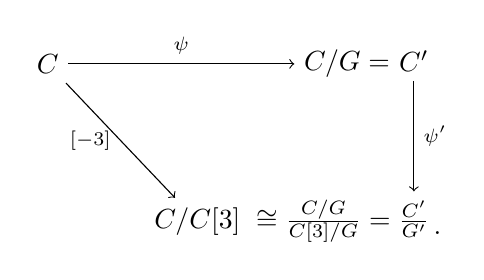
\begin{tikzpicture}[baseline=(current bounding box.center)]
          \node (LT) at (0, 2) {$C$}; 
          \node (MT) at (3.8, 2) {$C/G = $}; 
          \node (RT) at (4.65, 2.04) {$C'$}; 
          \node (LB) at (1.9, 0) {$C/C[3]$}; 
          \node (MB) at (3.5, 0) {$\cong \frac{C/G}{C[3]/G} = $}; 
          \node (RB) at (4.65, 0.025) {$\frac{C'}{G'}$}; 
          \node at (4.95, -0.15) {.}; 
          \draw [->] (LT) -- node [above] {$\scriptstyle \psi$} (MT); 
          \draw [->] (LT) -- node [left] {$\scriptstyle [-3]$} (LB); 
          \draw [->] (RT) -- node [right] {$\scriptstyle \psi'$} (RB); 
  \end{tikzpicture}
 \end{equation}
\end{prop}
\begin{proof}
 By Corollary \ref{cor:rig}, since $\Proj \s_3$ is connected, we need 
 only show that the locus over which $\psi' \circ \psi = [-3]$ is not 
 empty, where by abuse of notation $[-3]$ denotes the map $[-3]$ on $C$ 
 composed with the canonical isomorphism from $C/C[3]$ to $C'/G'$.  

 We have seen in Example \ref{ex:DF} that both $\psi$ and $\psi'$ 
 restrict as the 3-power Frobenius endomorphism $\psi_0$ of $C_0$.  By 
 \eqref{poly}, in the endomorphism ring of $C_0$, $\psi_0$ is a root of 
 the polynomial 
 \begin{equation}
 \label{charpoly}
  X^2 - \tr(\psi_0) \cdot X + 3 
 \end{equation}
 with $\tr(\psi_0)$ an integer satisfying 
 \begin{equation}
 \label{charineq}
  \big( \tr(\psi_0) \big)^2 \leq 12.  
 \end{equation}
 Moreover by \eqref{ssing}, since $C_0$ is supersingular, we have 
 \[
  \psi_0 \circ \psi_0 \equiv 0 \md 3, 
 \]
 and thus by \cite[12.3.3(1)]{KM} 
 \[
  \Hpsi_0 \circ \Hpsi_0 \equiv 0 \md 3.  
 \]
 We then have 
 \begin{equation*}
 \begin{split}
  \big( \tr(\psi_0) \big)^2 = & ~ (\psi_0 + \Hpsi_0) \circ (\psi_0 + \Hpsi_0) \\
                            = & ~ \psi_0 \circ \psi_0 + \Hpsi_0 \circ \psi_0 + \psi_0 \circ \Hpsi_0 + \Hpsi_0 \circ \Hpsi_0 \\
                            = & ~ \psi_0 \circ \psi_0 + 3 + 3 + \Hpsi_0 \circ \Hpsi_0 \\
                       \equiv & ~ 0 \md 3.  
 \end{split}
 \end{equation*}
 This congruence and \eqref{charineq} imply that $\tr(\psi_0) = 0$, 3, 
 or $-3$.  We exclude the latter two possibilities by checking the 
 action of $\psi_0$ at the 2-torsion point $(1,0)$ on 
 \[
  C_0 \co y^2 + x y - y = x^3 - x^2.  
 \]
 It then follows from \eqref{charpoly} that $\psi_0 \circ \psi_0$ agrees 
 with $[-3]$ on $C_0$ over $\BF_3$.  
\end{proof}

Analogous to \isog{iv}, let $\K'$ be the element in $\s_3$ such that 
$(\psi')^*$ sends $du$ to $\K' du$.  Note that $|\K'| = -6$.  

\begin{cor}
\label{cor:K'}
 The following relations hold in $\s_3$: 
 \[
  b^4 \K \K' + 3 = 0 
 \]
 and 
 \[
  \K' = -\K^3 + \frac{6}{b^2} ~ \K - \frac{a^2 - 8 b}{b^4}.  
 \]
\end{cor}
\begin{proof}
 The isogenies in \eqref{frob^2} induce maps on relative cotangent 
 spaces at the identity.  By \isog{iv} we then have a commutative 
 diagram 
 \begin{center}
 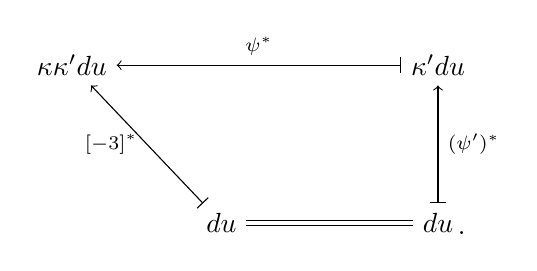
\begin{tikzpicture}
         \node (LT) at (0, 2) {$\K \K' du$}; 
         \node (RT) at (4.65, 2) {$\K' du$}; 
         \node (LB) at (1.9, 0) {$du$}; 
         \node (RB) at (4.65, 0) {$du$}; 
         \node at (4.95, -0.125) {.}; 
         \draw [|->] (RT) -- node [above] {$\scriptstyle \psi^*$} (LT); 
         \draw [|->] (LB) -- node [left] {$\scriptstyle [-3]^*$} (LT); 
         \draw [|->] (RB) -- node [right] {$\scriptstyle (\psi')^*$} (RT); 
         \draw [double distance=1.3pt] (LB) -- (RB); 
 \end{tikzpicture}
 \end{center}
 Thus for the first stated relation we need only show that $[3]^*$ sends 
 $du$ to $3 du / b^4$.  

 Let $P = (u,v)$ be a point on $C$.  For $i = 1$, 2, 3, and 4, let $Q_i$ 
 be a generator for each of the four degree-3 subgroups of $C$.  Each 
 $Q_i$ can be chosen as $Q$ in \eqref{u'v'}, and we denote the 
 corresponding quantity $\K$ in \eqref{KL} by $\K_i$.  Define an isogeny 
 $\Psi$ with source $C$ by 
 \begin{equation}
 \label{Psi}
 \begin{split}
  u\big( \Psi(P) \big) \ce & ~ u(P) \prod_{i=1}^4 \big( u(P-Q_i) \cdot u(P+Q_i) \big), \\
  v\big( \Psi(P) \big) \ce & ~ v(P) \prod_{i=1}^4 \big( v(P-Q_i) \cdot v(P+Q_i) \big).  
 \end{split}
 \end{equation}
 In view of \eqref{norm}, since $[3]$ has the same kernel as $\Psi$, we 
 have 
 \begin{equation}
 \label{s}
  [3]^* (du) = s \cdot \K_1 \K_2 \K_3 \K_4 \cdot du 
 \end{equation}
 where $s$ is a degree-0 unit in $\s$ coming from an automorphism of $C$ 
 over $\s$.  In view of \eqref{W} we have 
 \[
  \K_1 \K_2 \K_3 \K_4 = -\frac{3}{b^4}.  
 \]
 We compute that $s = -1$ by comparing the restrictions of the two sides 
 of \eqref{s} to the point corresponding to the homogeneous maximal 
 ideal $(5,H)$ of $\s$, and then comparing the restrictions to the point 
 corresponding to $(7,H)$.  Over both points, $[3]^*$ becomes the 
 multiplication-by-3 map, and $-3 / b^4$ becomes $-3$.  Thus $[3]^*$ 
 sends $du$ to $3 du / b^4$.  

 The second stated relation follows by a computation from the first 
 relation and the relation $W(\K) = 0$ as in \isog{i}.  
\end{proof}

\begin{rmk}
 As noted in Remark \ref{rmk:K}, the (local) analog of $\K$ at the prime 
 2 coincides with the parameter $d$ in \cite[Section 3]{h2p2}.  In 
 particular, with the notations there and the equation in 
 \cite[Proposition 3.2]{tmf3}, $d$ and $d'$ satisfy an analogous 
 relation $A_3 d d' + 2 = 0$ which locally reduces to $d d' + 2 = 0$.  
 These arise as examples of \cite[Lemma 3.21]{poonen}.  
\end{rmk}

\begin{rmk}
 In view of \eqref{frob^2}, $-\psi'$ (composed with the canonical 
 isomorphism on the target) turns out to be the dual isogeny of $\psi$ 
 (cf.~the proof of \cite[2.9.4]{KM}).  If $G$ is the unique degree-3 
 subgroup of $C$ in a formal neighborhood of the identity, then 
 \begin{equation}
 \label{Kmod3}
  \K \equiv 0 \md 3 
 \end{equation}
 by \eqref{dmod3} and \eqref{K}.  Thus in view of Corollary 
 \ref{cor:K'} and \eqref{H} we have 
 \[
  -\K' = \K^3 - \frac{6}{b^2} ~ \K + \frac{a^2 - 8 b}{b^4} 
  \equiv \frac{H}{b^4} \md 3.  
 \]
 This congruence agrees with the interpretation of $H$ as defined by the 
 tangent map of the Verschiebung isogeny over $\BF_3$ (see Section 
 \ref{subsec:fg}).  
\end{rmk}

\subsubsection*{Isogenies as studied by Lubin and V\'elu}

The isogeny $\Psi$ in the proof of Corollary \ref{cor:K'} above and the 
isogeny $\psi$ in Proposition \ref{prop:isog} (cf.~\eqref{Psi} and 
\eqref{u'v'}) are examples of a construction used by Lubin in his study 
of finite isogenies of formal groups.  

\begin{thm}[Lubin, see {\cite[Theorem 1.4]{lubin}}]
\label{thm:lubin}
 Let $p$ be a prime number.  Let $k$ be a finite extension of $\BQ_p$, 
 and $K$ a finite extension of $k$.  Denote by $\CO_k$ and $\CO_K$ the 
 rings of integers in $k$ and $K$ respectively.  Let $\G$ be a formal 
 group law over $\CO_k$, and $G$ a finite subgroup of $\G(\CO_K)$.  Then 
 there is a formal group law $\G'$ defined over $\CO_K$ and a 
 $\phi \in \Hom_{\CO_K}(\G,\G')$ with $\ker \phi = G$.  Moreover, if $G$ 
 is stable under the action of $\Aut(\ck/k)$, then $\G'$ can be defined 
 over $\CO_k$.  
\end{thm}

In the proof of this theorem, Lubin gives explicitly the function $\phi$ 
as 
\begin{equation}
\label{lubin}
 \phi(x) = \prod_{g \in G} (x +_\G g) \in \CO_K \llbracket x \rrbracket.  
\end{equation}

\begin{rmk}
 In \cite{Ando95} Ando constructs coordinates on certain Lubin-Tate 
 formal groups which are preserved under isogenies (see 
 \cite[Theorem 2.5.7]{Ando95}).  The problem addressed by his theorem 
 arose in the study of cohomology operations in elliptic cohomology and 
 Morava $E$-theories.  In particular, with notations as in Theorem 
 \ref{thm:lubin}, his coordinate $x$ is determined by requiring that the 
 corresponding formal group law $\G$ satisfy 
 \[
  \phi(x) = [p](x) 
 \]
 for $G$ the subgroup of $p$-torsion points (see 
 \cite[Theorem 2.6.4]{Ando95}).  When the formal group is $\HC$ and 
 $p=3$, with notations as in the proof of Corollary \ref{cor:K'}, the 
 above identity becomes 
 \[
  x\big( \Psi(P) \big) = x\big( [3](P) \big) 
 \]
 which our coordinate $u$ does not satisfy (recall that we have 
 $s = -1$).  On the other hand, in the prime-2 case studied by Rezk in 
 \cite{h2p2}, this holds for the analogous coordinate $u$.  
\end{rmk}

Constructions similar to \eqref{lubin} appear in the study of finite 
subgroups and isogenies of elliptic curves.  For an elliptic curve $E$ 
over a field of characteristic not equal to 2 or 3, the division 
polynomials in Definition \ref{def:division} are given by 
\begin{equation}
\label{division}
 \psi_m(x) = \prod_{Q \in (E[m]-\{O\}) / \{\pm1\}} \big( x - x(Q) \big) 
\end{equation}
(see \cite[13(9.2)]{husemoller}).  Since $E[m]-\{O\}$ is stable under 
the automorphism $[-1]$ on $E$ which fixes $x$, it is defined by the 
equation $\psi_m(x) = 0$.  

Using a polynomial in $x$ that defines a finite subgroup, we can compute 
an isogeny whose kernel is this subgroup.  The formulas are given by 
V\'elu \cite{velu}.  

Let $E$ be an elliptic curve over an algebraically closed field given by 
a Weierstrass equation \eqref{xy} in $xy$-coordinates.  Let $P = (x,y)$ 
be a point on $E$.  Let $G$ be a finite subgroup of $E$, and denote by 
$E'$ the quotient curve $E/G$.  Define an isogeny $\Phi \co E \to E'$ by 
\begin{equation}
\label{velu}
\begin{split}
 x \big( \Phi(P) \big) \ce & ~ x(P) + \sum_{Q \in G-\{O\}} \big( x(P+Q) - x(Q) \big), \\
 y \big( \Phi(P) \big) \ce & ~ y(P) + \sum_{Q \in G-\{O\}} \big( y(P+Q) - y(Q) \big).  
\end{split}
\end{equation}
V\'elu gives an explicit Weierstrass equation of $E'$ with coefficients 
in terms of the coordinates of the points $Q$ in $G-\{O\}$.  

Below we follow the presentation of V\'elu's formulas in 
\cite[Section 2.4]{kohel} in terms of a polynomial $\psi(x)$ defining 
$G-\{O\}$ (cf.~\cite{dewaghe}).  As we mentioned above for $\psi_m(x)$ 
in \eqref{division} defining $E[m]-\{O\}$, such a polynomial exists as 
$x$ is fixed by the automorphism $[-1]$ on $E$.  We discuss only the 
case when the degree $d$ of $G$ is odd and the base field is of 
characteristic not equal to 2.  

Write $d = 2 n + 1$ and $s_i$ the $i$'th elementary symmetric function 
in the roots of $\psi(x)$ so that 
\[
 \psi(x) = x^n - s_1 x^{n-1} + \cdots + (-1)^n s_n.  
\]
Write $\psi_2 = 2 y + a_1 x + a_3$ as in Definition \ref{def:division}.  
The isogeny $\Phi$ is given by 
\[
 \Phi(x,y) = \left( \frac{\phi(x)}{\psi(x)^2}, 
 \frac{\omega(x,y)}{\psi(x)^3} \right) 
\]
(cf.~\eqref{[m]}) where 
\begin{equation*}
\begin{split}
     \phi(x) = & ~ (4 x^3 + b_2 x^2 + 2 b_4 x + b_6) \big( \psi'(x)^2 - \psi''(x) \psi(x) \big) \\
               & ~ - (6 x^2 + b_2 x + b_4) \psi'(x) \psi(x) + (d x - 2 s_1) \psi(x)^2, \\
 \omega(x,y) = & ~ \phi'(x) \psi(x) \psi_2 / 2 - \phi(x) \psi'(x) \psi_2 - \big( a_1 \phi(x) + a_3 \psi(x)^2 \big) \psi(x) / 2.  
\end{split}
\end{equation*}
The equation of the quotient curve $E'$ is given by 
\[
 y^2 + a_1 x y + a_3 y = x^3 + a_2 x^2 + (a_4 - 5 t) x + a_6 - b_2 t 
 - 7 w 
\]
where 
\begin{equation*}
\begin{split}
 t = & ~ 6 (s_1^2 - 2 s_2) + b_2 s_1 + n b_4, \\
 w = & ~ 10 (s_1^3 - 3 s_1 s_2 + 3 s_3) + 2 b_2 (s_1^2 - 2 s_2) + 3 b_4 s_1 + n b_6.  
\end{split}
\end{equation*}

As an application of V\'elu's formulas, we give an alternate 
computation, in $xy$-coordinates, of the universal degree-3 isogeny 
$\psi$ in Proposition \ref{prop:isog}.  

\begin{ex}
\label{ex:velu}
 We continue with the notations in Proposition \ref{prop:isog} and 
 V\'elu's formulas above.  Let $s$ be the $x$-coordinate of the 
 3-torsion point $Q$ on $C$, with $|s| = 2$.  As in \eqref{psi_3}, it 
 satisfies 
 \begin{equation}
 \label{TW}
  \TW(s) \ce 3 s^4 + (a^2 + 4 b) s^3 + 3 a^2 b s^2 + 3 a^2 b^2 s 
  + a^2 b^3 = 0.  
 \end{equation}
 Since the $x$-coordinate of any point on $C$ is fixed by $[-1]$, which 
 is the only nontrivial automorphism of any degree-3 subgroup, we then 
 have 
 \[
  \s_3 \cong \s [s] \big/ \big( \TW(s) \big).  
 \]

 Let $G$ be the subgroup generated by $Q$.  The universal degree-3 
 isogeny 
 \[
  \psi \co C \longrightarrow C' = C/G 
 \]
 is determined up to an isomorphism by the polynomial (with an abuse of 
 notation) 
 \[
  \psi(x) \ce x - s, 
 \]
 as the point $-Q$ has the same $x$-coordinate as $Q$.  We have $d = 3$ 
 and $n = 1$, and in the identity 
 \[
  \psi(x) = x^n - s_1 x^{n-1} + \cdots + (-1)^n s_n 
 \]
 we have 
 \[
  s_1 = s, \qquad \ad \qquad s_i = 0 \quad \text{for} \quad i > 1.  
 \]
 We then compute that 
 \begin{equation*}
 \begin{split}
      \phi(x) = & ~ x^3 - 2 s x^2 + (7 s^2+ a^2 s + 4 b s + a^2 b) x - 2 s^3 + a^2 b s + a^2 b^2, \\
  \omega(x,y) = & ~ \big( x^3 - 3 s x^2 + (-3 s^2 - a^2 s - 4 b s - a^2 b) x - 3 s^3 - a^2 s^2 - 4 b s^2 - 3 a^2 b s \\
                & ~ - 2 a^2 b^2 \big) y + (-6 a s^2 - a^3 s - 4 a b s - a^3 b) x^2 + (3 a s^3 - 3 a b s^2 -2 a^3 b s \\
                & ~ - 2 a b^2 s - 2 a^3 b^2) x - a s^4 - a b s^3 - 2 a b^2 s^2 - a^3 b^2 s - a^3 b^3.  
 \end{split}
 \end{equation*}
 In view of \eqref{TW}, the 4-torsion point $(0,0)$ on $C$ (see Example 
 \ref{ex:C}) then maps to 
 \[
  (x_0, y_0) \ce \left( \frac{\phi(0)}{\psi(0)^2}, 
  \frac{\omega(0,0)}{\psi(0)^3} \right) 
 \]
 where 
 \begin{equation*}
 \begin{split}
  x_0 = & ~ 6 b^{-2} s^3 + (2 a^2 b^{-2} + 5 b^{-1}) s^2 + (5 a^2 b^{-1} - 6) s + 3 a^2, \\
  y_0 = & ~ (-9 a b^{-2} - 6 a^{-1} b^{-1}) s^3 + (-3 a^3 b^{-2} - 8 a b^{-1} - 8 a^{-1}) s^2 - 7 a^3 b^{-1} s \\
        & ~ - 4 a^3 - 9 a b.  
 \end{split}
 \end{equation*}

 The equation of the quotient curve is given by 
 \[
  y^2 + a x y + a b y = x^3 + b x^2 - 5 t x - (a^2 + 4 b) t - 7 w 
 \]
 where 
 \begin{equation*}
 \begin{split}
  t = & ~ 6 s^2 + (a^2 + 4 b) s + a^2 b, \\
  w = & ~ 10 s^3 + (2 a^2 + 8 b) s^2 + 3 a^2 b s + a^2 b^2.  
 \end{split}
 \end{equation*}
 We normalize this equation into the form of \eqref{Cxy} by making two 
 changes of variables, where $x'$ and $y'$ are the variables after each 
 change: 
 \begin{itemize}
  \item set 
  \[
   x = x' + x_0 \qquad \ad \qquad y = y' + y_0; 
  \]

  \item set 
  \[
   \qquad x = x' \qquad \ad \qquad y = y' + k x \thinspace
  \]
  where 
  \[
   k = -6 a^{-1} b^{-2} s^3 + (-2 a b^{-2} - 8 a^{-1} b^{-1}) s^2 
   - 6 a b^{-1} s - 5 a.  
  \]
 \end{itemize}
 We then have 
 \[
  C' \co y^2 + a' x y + a' b' y = x^3 + b' x^2 
 \]
 where 
 \begin{equation*}
 \begin{split}
  a' = & -\frac{1}{a b^2} \big( 12 s^3 + (4 a^2 + 16 b) s^2 + 12 a^2 b s + 9 a^2 b^2 \big), \\
  b' = & ~ \frac{1}{b} \big( 3 s^2 + (a^2 - 2 b) s + a^2 b + b^2 \big).  
 \end{split}
 \end{equation*}
 Since $|a'| = |a| = 1$ and $|b'| = |b| = 2$ (cf.~\eqref{a'b'K}), the 
 isogeny $C \to C'$ computed above cannot be a deformation of the 
 3-power Frobenius endomorphism over the supersingular locus at the 
 prime 3 (see Remark \ref{rmk:DF}).  To get a deformation of Frobenius, 
 we need a further change of variables: 
 \begin{itemize}
  \item set 
  \[
   x = \lambda^{-2} x' \qquad \ad \qquad y = \lambda^{-3} y' ~
  \]
  where 
  \[
   \lambda = -s - b.  
  \]
 \end{itemize}
 We will write the equation of the resulting curve in terms of a new 
 parameter $\T \ce 1/s$, with $|\T| = -2$ and 
 \begin{equation}
 \label{TTW}
  a^2 b^3 \T^4 + 3 a^2 b^2 \T^3 + 3 a^2 b \T^2 + (a^2 + 4 b) \T + 3 = 0 
 \end{equation}
 in $\s_3$ (cf.~\eqref{TW}).  In view of Proposition \ref{prop:tors}, 
 since $\T = e/d$, we compute that 
 \begin{equation}
 \label{T}
 \begin{split}
  \T = & ~ \frac{1}{a (a^2 - 16 b)} \big( 6 b^4 d^7 + 17 a b^3 d^6 + (15 a^2 b^2 + 2 b^3) d^5 + (3 a^3 b \\
       & + 48 a b^2) d^4 + (-a^4 + 35 a^2 b - 38 b^2) d^3 +(-4 a^3 + 69 a b) d^2 \\
       & + (-6 a^2 + 30 b) d - 6 a \big).  \\
 \end{split}
 \end{equation}
 In particular, if $Q$ is in a formal neighborhood of the identity, then 
 by \eqref{dmod3} we have 
 \[
  \T \equiv 0 \md 3.  
 \]
 Now, after the final change of variables, $a'$ and $b'$ become 
 \begin{equation}
 \label{a'b'T}
 \begin{split}
  a' = & ~ a \big( a^2 b^3 \T^3 + 3 a^2 b^2 \T^2 + (3 a^2 b - 4 b^2) \T + a^2 - 3 b \big), \\
  b' = & ~ b^3, 
 \end{split}
 \end{equation}
 which reduce to $a' = a^3$ and $b' = b^3$ over the supersingular locus, 
 and thus we get a deformation of Frobenius.  In view of \eqref{K}, 
 \eqref{T}, and \eqref{f}, we have a relation 
 \[
  (b \K + 1) (b \T + 1) = 1 
 \]
 in the ring $\s [d] \big/ \big( f(d) \big)$.  We then check that 
 \eqref{a'b'K} and \eqref{a'b'T} agree via this relation.  Thus we 
 recover the computation of the universal degree-3 isogeny 
 $\psi \co C \to C'$ in Proposition \ref{prop:isog} using V\'elu's 
 formulas and the parameter $\T$.  
\end{ex}

\begin{rmk}
 As the group law on the elliptic curve is encoded in V\'elu's formulas, 
 the computation of $\psi$ in Example \ref{ex:velu} above is 
 considerably easier than the one in Proposition \ref{prop:isog}.  
 However, for our purpose of studying power operations, this second 
 approach is less convenient, as the construction \eqref{velu} is not a 
 priori a deformation of Frobenius.  In fact we have to compose an 
 isomorphism as in the changes of variables toward the end of the 
 computation.  In general, Lubin's and V\'elu's constructions define 
 isogenies which have the same kernel but differ by an isomorphism.  

 In V\'elu's construction, the invariant one-form $\omega$ defined in 
 \eqref{quantities} on $E'$ pulls back along $\Phi$ to that on $E$ (see 
 \cite[Remarque 2]{velu}).  This property does not hold in Lubin's 
 construction.  In fact, over the supersingular locus the induced map 
 on the relative cotangent space at the identity is zero (see Theorem 
 \ref{thm:igusa}).  

 An important property of Lubin's and V\'elu's constructions is that 
 they are both functorial under composition of isogenies (see 
 \cite[Proposition 2.2.6]{Ando95} and \cite[Section 2.4]{kohel}).  
\end{rmk}

\begin{rmk}
 We can rewrite \eqref{TTW} as 
 \begin{equation}
 \label{charles}
  b^4 \T \T' + 3 = 0 
 \end{equation}
 where 
 \[
  \T' = \frac{a^2}{b} ~ \T^3 + \frac{3 a^2}{b^2} ~ \T^2 
  + \frac{3 a^2}{b^3} ~ \T + \frac{a^2 + 4 b}{b^4}.  
 \]
 However, unlike in Corollary \ref{cor:K'}, $\T'$ is not the parameter 
 analogous to $\T$ for the isogeny $\psi'$.  In particular, the relation 
 \eqref{TTW} no longer holds in $\s_3$ if we substitute $a$, $b$, and 
 $\T$ by $a'$, $b'$, and $\T'$ respectively.  
\end{rmk}


\subsection{Moduli problems}
\label{subsec:mp}

Individual finite subgroups and isogenies of elliptic curves determine 
various types of ``level structures'' on the elliptic curves.  We can 
study them systematically, each type as a whole, by studying the 
corresponding moduli problems.  Based on Definitions \ref{def:cyclic} 
and \ref{def:cso}, we first define these level structures in the sense 
of Drinfeld (cf.~\cite[3.1-4 and 7.9.4]{KM}).  

\begin{defn}
\label{def:level}
 Let $S$ be a scheme, $E/S$ an elliptic curve, and $m \geq 1$ an 
 integer.  
 \begin{enumerate}[(i)]
  \item A {\em $\G(m)$-structure} on $E/S$ is a pair of points $(P,Q)$ 
  on $E$ which generate $E[m]$, i.e., we have an equality of effective 
  Cartier divisors in $E$: 
  \[
   E[m] = \sum_{i,~j {~\rm mod~} m} [iP + jQ].  
  \]

  \item A {\em $\G_1(m)$-structure} on $E/S$ is a point $P$ on $E$ which 
  has exact order $m$, i.e., the effective Cartier divisor 
  \[
   \sum_{i {~\rm mod~} m} [iP] 
  \]
  is a subgroup scheme of $E$.  

  \item A {\em balanced $\G_1(m)$-structure} on $E/S$ is a diagram 
  \begin{center}
  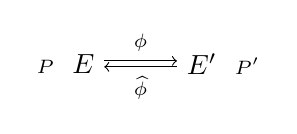
\begin{tikzpicture}
          \node (L) at (0, 0) {${\scriptstyle P}~~E$}; 
          \node (R) at (2, 0) {$E'~~{\scriptstyle P'}$}; 
          \draw [transform canvas={yshift=0.25ex},->] (L) -- node [above] {$\scriptstyle \phi$} (R); 
          \draw [transform canvas={yshift=-0.25ex},<-] (L) -- node [below] {$\scriptstyle \Hphi$} (R); 
  \end{tikzpicture}
  \end{center}
  where $E'$ is an elliptic curve over $S$, $\phi$ is a degree-$m$ 
  isogeny, $\Hphi$ is the dual isogeny, $P \in (\ker \phi)(S)$ is a 
  generator of $\ker \phi$, and $P' \in (\ker \Hphi)(S)$ is a generator 
  of $\ker \Hphi$.  

  \item \label{level(iv)} A {\em $\G_0(m)$-structure} on $E/S$ is a 
  degree-$m$ isogeny 
  \[
   E \stackrel{\phi}{\longrightarrow} E' = E/G 
  \]
  of elliptic curves over $S$ where $G = \ker \phi$ is cyclic.  

  \item Suppose $m = p^n$ for some prime $p$ and integer $n$.  Let 
  $0 \leq a,b \leq n$ be integers.  A {\em $[\G_0(p^n);a,b]$-structure} 
  on $E/S$ is a diagram 
  \begin{center}
  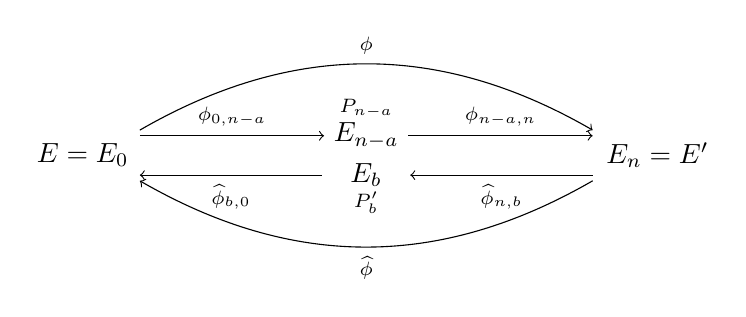
\begin{tikzpicture}
          \node (L) at (-0.6, 0) {$E = E_0$}; 
          \node (R) at (6.7, 0) {$E_n = E'$}; 
          \node (LT) at (0, 0.25) {$ $}; 
          \node (RT) at (6, 0.25) {$ $}; 
          \node (LB) at (0, -0.25) {$ $}; 
          \node (RB) at (6, -0.25) {$ $}; 
          \node (MT) at (3, 0.25) {$E_{n-a}$}; 
          \node (MB) at (3, -0.25) {$~~E_b~~$}; 
          \node (MTT) at (3, 0.6) {$\scriptstyle P_{n-a}$}; 
          \node (MBB) at (3, -0.6) {$\scriptstyle P'_b$}; 
          \draw [->] (LT) -- node [above] {$\scriptstyle \phi_{0,n-a}$} (MT); 
          \draw [<-] (LB) -- node [below] {$\scriptstyle \Hphi_{b,0}$} (MB); 
          \draw [<-] (RT) -- node [above] {$\scriptstyle \phi_{n-a,n}$} (MT); 
          \draw [->] (RB) -- node [below] {$\scriptstyle \Hphi_{n,b}$} (MB); 
          \draw [->] (LT) to [out = 30, in = 150] node [above] {$\scriptstyle \phi$} (RT); 
          \draw [<-] (LB) to [out = -30, in = -150] node [below] {$\scriptstyle \Hphi$} (RB); 
  \end{tikzpicture}
  \end{center}
  where $E'$ is an elliptic curve over $S$, $\phi$ is a degree-$p^n$ 
  isogeny, $\Hphi$ is the dual isogeny, $(\phi_{0,n-a},\phi_{n-a,n})$ is 
  a pair of isogenies cyclic in standard order with $\phi_{n-a,n}$ of 
  degree $p^a$, $(\Hphi_{n,b},\Hphi_{b,0})$ is a pair of isogenies 
  cyclic in standard order with $\Hphi_{b,0}$ of degree $p^b$, 
  $P_{n-a} \in (\ker \phi_{n-a,n})(S)$ is a generator of 
  $\ker \phi_{n-a,n}$, and $P'_b \in (\ker \Hphi_{b,0})(S)$ is a 
  generator of $\ker \Hphi_{b,0}$.  
 \end{enumerate}
\end{defn}

The notion of a moduli problem for elliptic curves provides a way to 
parametrize these structures.  To introduce the definition, we note that 
our setting here is comparable, and indeed related, to that for 
deformations of Frobenius in Section \ref{subsec:bridge}.  

\begin{defn}[cf.~Definition \ref{def:DF}]
 For any scheme $S$, let $\Ell(S)$ be the category whose objects are 
 elliptic curves over $S$, and whose morphisms are $S$-homomorphisms.  
 In particular, for any ring $R$, we write $\Ell(R) \ce \Ell(\Spec R)$.  
\end{defn}

Note that for a fixed ring $R$, $\Ell(R)$ is the category $\CA$ in 
Theorem \ref{thm:serretate}, and is different from the category $\Ell/R$ 
in Definition \ref{def:mpR} below.  

\begin{defn}[cf.~Definition \ref{def:mod}]
\label{def:mp}
 We write $\Ell \ce \{ \Ell(S) \}$.  Precisely, $\Ell$ is the category 
 whose objects are elliptic curves 
 \begin{center}
 \begin{tikzpicture}
         \node (T) at (0, 2) {$E$}; 
         \node (B) at (0, 0) {$S$}; 
         \draw [->] (T) -- node [right] {$\scriptstyle \pi$} (B); 
 \end{tikzpicture}
 \end{center}
 over variable base schemes, and whose morphisms are cartesian squares 
 \begin{center}
 \begin{tikzpicture}
         \node (LT) at (0, 2) {$E_1$}; 
         \node (RT) at (3, 2) {$E$}; 
         \node (LB) at (0, 0) {$S_1$}; 
         \node (RB) at (3, 0) {$S$}; 
         \node at (3.25, -0.125) {,}; 
         \draw [->] (LT) -- node [above] {$\scriptstyle \phi$} (RT); 
         \draw [->] (LB) -- node [above] {$\scriptstyle f$} (RB); 
         \draw [->] (LT) -- node [left] {$\scriptstyle \pi_1$} (LB); 
         \draw [->] (RT) -- node [right] {$\scriptstyle \pi$} (RB); 
 \end{tikzpicture}
 \end{center}
 i.e., commutative squares such that the induced morphism of 
 $S_1$-schemes 
 \[
  E_1 \xrightarrow{(\phi,\pi_1)} E \times_S S_1 
 \]
 is an isomorphism of elliptic curves over $S_1$.  

 A {\em moduli problem $\CP$ (over $\Ell$)} is a functor 
 \[
  \CP \co \Ell^\op \longrightarrow \Set.  
 \]
 Morphisms between moduli problems are natural transformations.  
\end{defn}

We denote the moduli problems associated to the level structures in 
Definition \ref{def:level} by 
\begin{equation}
\label{five}
 [\G(m)], \quad [\G_1(m)], \quad [{\rm bal.} \thinspace \G_1(m)], 
 \quad [\G_0(m)], \quad [\G_0(p^n);a,b].  
\end{equation}
In general, given a moduli problem $\CP$ and an elliptic curve $E/S$, an 
element in the set $\CP(E/S)$ is called a {\em (level) $\CP$-structure 
on $E/S$}.  

\begin{defn}[{\cite[4.2]{KM}}]
 A moduli problem $\CP$ is said to be {\em relatively representable 
 (over $\Ell$)} if for every elliptic curve $E/S$, the functor on 
 $(\Sch/S)^\op$ defined on objects by 
 \[
  T \longmapsto \CP \big( (E \times_S T) / T \big) 
 \]
 is representable by an $S$-scheme denoted by $\CP_{E/S}$.  
\end{defn}

\begin{thm}[{\cite[5.1.1, 7.9.6, and 7.1.3(1)]{KM}}]
\label{thm:relrep}
 Each of the five moduli problems \eqref{five} is relatively 
 representable over $\Ell$.  
\end{thm}

\begin{defn}
 A moduli problem $\CP$ is said to be {\em representable} if it is 
 representable as a functor, i.e., if there exists an elliptic curve 
 over a scheme denoted by 
 \begin{center}
 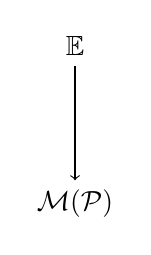
\begin{tikzpicture}
         \node (T) at (0, 2) {$\BE$}; 
         \node (B) at (0, 0) {$\CM(\CP)$}; 
         \draw [->] (T) -- (B); 
 \end{tikzpicture}
 \end{center}
 together with a functorial isomorphism 
 \[
  \CP(E/S) \cong \Hom_\Ell \big( E/S, \BE/\CM(\CP) \big).  
 \]
\end{defn}

Any representable moduli problem is relatively representable (see 
\cite[4.3.2]{KM}).  

Given moduli problems $\CP$ and $\CP'$, the {\em simultaneous moduli 
problem $(\CP,\CP')$} is the moduli problem defined on objects by 
\[
 E/S \longmapsto \CP(E/S) \times \CP'(E/S).  
\]
If $\CP$ is representable and $\CP'$ is relatively representable, then 
$(\CP,\CP')$ is representable, and we have 
\[
 \CM(\CP,\CP') = \CP'_{\BE/\CM(\CP)} 
\]
where $\BE/\CM(\CP)$ represents $\CP$.  

Given a representable moduli problem $\CP$, the scheme $\CM(\CP)$ 
represents the functor on $\Sch$ which sends a scheme $S$ to the set 
\[
 \left\{
  \begin{array}{l}
   \text{isomorphism classes of pairs $(E/S,x)$ with} \\
   \quad \text{$E$ an elliptic curve over $S$ and} \\
   \quad \text{$x \in \CP(E/S)$ a $\CP$-structure on $E/S$} 
  \end{array}
 \right\}.  
\]
Motivated by this, we give the following definition of a more general 
class of morphisms between moduli problems.  It allows the flexibility 
to consider isomorphism classes, rather than individual objects, of 
elliptic curves equipped with level structures.  In particular, such a 
morphism between two representable moduli problems induces a morphism of 
their representing moduli schemes, free of reference to the universal 
elliptic curves over these schemes (see Examples \ref{ex:ab4} and 
\ref{ex:ab3}).  

\begin{defn}
\label{def:abstract}
 An {\em abstract morphism $\CP \to \CP'$ of moduli problems} is a rule 
 which to every scheme $S$ and every elliptic curve $E/S$ with 
 $\CP$-structure $x \in \CP(E/S)$, assigns an elliptic curve $E'/S$ with 
 $\CP'$-structure $x' \in \CP'(E'/S)$, and which to every morphism 
 \begin{center}
 \begin{tikzpicture}
         \node (LT) at (0, 2) {$E_1$}; 
         \node (RT) at (3, 2) {$E$}; 
         \node (LB) at (0, 0) {$S_1$}; 
         \node (RB) at (3, 0) {$S$}; 
         \node (B)  at (5.85, 0) {$ $}; 
         \node (L)  at (-2,2) {$\scriptstyle x_1 = (\phi,~f)^*(x) \in \CP(E_1/S_1)$}; 
         \node (R)  at (4, 2) {$\scriptstyle x \in \CP(E/S)$}; 
         \draw [->] (LT) -- node [above] {$\scriptstyle \phi$} (RT); 
         \draw [->] (LB) -- node [above] {$\scriptstyle f$} (RB); 
         \draw [->] (LT) -- (LB); 
         \draw [->] (RT) -- (RB); 
 \end{tikzpicture}
 \end{center}
 in $\Ell$ assigns a morphism 
 \begin{center}
 \begin{tikzpicture}
         \node (LT) at (0, 2) {$E_1'$}; 
         \node (RT) at (3, 2) {$E'$}; 
         \node (LB) at (0, 0) {$S_1$}; 
         \node (RB) at (3, 0) {$S$}; 
         \node (L)  at (-1.5,2) {$\scriptstyle (x_1)' \in \CP'(E_1'/S_1)$}; 
         \node (R)  at (4.1, 2) {$\scriptstyle x' \in \CP'(E'/S)$}; 
         \draw [->] (LT) -- node [above] {$\scriptstyle \phi'$} (RT); 
         \draw [->] (LB) -- node [above] {$\scriptstyle f$} (RB); 
         \draw [->] (LT) -- (LB); 
         \draw [->] (RT) -- (RB); 
 \end{tikzpicture}
 \end{center}
 with the same $f$, such that 
 \[
  (x_1)' = (\phi',~f)^*(x'), 
 \]
 and such that the assignment $(\phi,~f) \mapsto (\phi',~f)$ is 
 compatible with composition of morphisms in $\Ell$.  
\end{defn}

In particular, the rule of an abstract morphism $\CP \to \CP'$ sends an 
isomorphism 
\begin{center}
\begin{tikzpicture}
        \node (LT) at (0, 2) {$E_1$}; 
        \node (RT) at (3, 2) {$E$}; 
        \node (LB) at (0, 0) {$S$}; 
        \node (RB) at (3, 0) {$S$}; 
        \node (B)  at (-4.25, 0) {$ $}; 
        \node (L)  at (-2,2) {$\scriptstyle x_1 = (\phi,~\id_S)^*(x) \in \CP(E_1/S)$}; 
        \node (R)  at (5, 2) {$\scriptstyle x = (\phi^{-1},~\id_S)^*(x_1) \in \CP(E/S)$}; 
        \draw [transform canvas={yshift=0.25ex},->] (LT) -- node [above] {$\scriptstyle \phi$} (RT); 
        \draw [transform canvas={yshift=-0.25ex},<-] (LT) -- node [below] {$\scriptstyle \phi^{-1}$} (RT); 
        \draw [double distance=1.3pt] (LB) -- (RB); 
        \draw [->] (LT) -- (LB); 
        \draw [->] (RT) -- (RB); 
\end{tikzpicture}
\end{center}
to an isomorphism 
\begin{center}
\begin{tikzpicture}
        \node (LT) at (0, 2) {$E_1'$}; 
        \node (RT) at (3, 2) {$E'$}; 
        \node (LB) at (0, 0) {$S$}; 
        \node (RB) at (3, 0) {$S$}; 
        \node (B)  at (-5.25, 0) {$ $}; 
        \node (L)  at (-2.3,2) {$\scriptstyle (x_1)' = (\phi',~\id_S)^*(x') \in \CP'(E_1'/S)$}; 
        \node (R)  at (5.5, 2) {$\scriptstyle x' = \big( (\phi')^{-1},~\id_S \big)^*\big( (x_1)' \big) \in \CP'(E'/S)$}; 
        \node at (3.25, -0.125) {.}; 
        \draw [transform canvas={yshift=0.25ex},->] (LT) -- node [above] {$\scriptstyle \phi'$} (RT); 
        \draw [transform canvas={yshift=-0.25ex},<-] (LT) -- node [below] {$\scriptstyle (\phi')^{-1}$} (RT); 
        \draw [double distance=1.3pt] (LB) -- (RB); 
        \draw [->] (LT) -- (LB); 
        \draw [->] (RT) -- (RB); 
\end{tikzpicture}
\end{center}
Thus, if both $\CP$ and $\CP'$ are representable, passing to isomorphism 
classes the abstract morphism $\CP \to \CP'$ then induces a morphism 
$\CM(\CP) \to \CM(\CP')$ of schemes.  

\begin{rmk}
 A morphism $\CP \to \CP'$ (see Definition \ref{def:mp}) is an abstract 
 morphism which to every scheme $S$ and every elliptic curve $E/S$ with 
 $\CP$-structure $x \in \CP(E/S)$, assigns the {\em same} $E/S$ with 
 $\CP'$-structure $x' \in \CP'(E/S)$, and which to every morphism 
 $(\phi,~f)$ in $\Ell$ assigns the {\em same} $(\phi,~f)$.  
\end{rmk}

The definition of a moduli problem over the category $\Ell$ in 
Definition \ref{def:mp} and the related notions we have discussed 
thereafter generalize to the following category.  

\begin{defn}[cf.~Definition \ref{def:mp}]
\label{def:mpR}
 For any ring $R$, let $\Ell/R$ be the category of elliptic curves over 
 variable $R$-schemes, with morphisms the cartesian squares whose bottom 
 arrow is $R$-linear.  
\end{defn}

\begin{thm}[{\cite[3.7.1, 7.9.6, and 7.1.3(2)]{KM}}]
\label{thm:affine}
 Each of the five moduli problems \eqref{five}, as a relatively 
 representable moduli problem over $\Ell/\BZ[1/m]$ via the forgetful map 
 $\Ell/\BZ[1/m] \to \Ell$, is finite \'etale over $\Ell/\BZ[1/m]$, i.e., 
 for every elliptic curve $E/S/\BZ[1/m]$, the morphism 
 \begin{center}
 \begin{tikzpicture}
         \node (T) at (0, 2) {$\CP_{E/S}$}; 
         \node (B) at (0, 0) {$S$}; 
         \draw [->] (T) -- (B); 
 \end{tikzpicture}
 \end{center}
 is finite \'etale if $\CP$ is any of these moduli problems.  
\end{thm}

Representability of the moduli problems \eqref{five} is more delicate.  
It involves the {\em rigidity} of a moduli problem, i.e., the property 
that the automorphism group of any elliptic curve acts freely on the set 
of level structures on the elliptic curve (see 
\cite[4.4, 4.7, and 2.7]{KM}).  For example, $[\G_1(m)]$ over 
$\Ell/\BZ[1/m]$ is rigid if $m \geq 4$ by \cite[2.7.3]{KM}, and thus 
combined with its relative representability from Theorem 
\ref{thm:relrep} and affineness from Theorem \ref{thm:affine} it is 
representable over $\Ell/\BZ[1/m]$ by \cite[4.7.0]{KM}.  

Another example is the moduli problem $[\omega]$ defined on objects by 
\[
 [\omega](E/S) \ce \{ \text{nowhere-vanishing invariant one-forms on} 
 ~ E/S \}.  
\]
It is relatively representable over $\Ell$, but not representable (see 
\cite[8.1.7.1]{KM}).  

In practice, even if we know by general representability results that a 
moduli problem $\CP$ is representable, we may not be able to work with 
$\CM(\CP)$ explicitly.  It is often interesting to consider simultaneous 
moduli problems $(\CP,\CP')$ and restrictions of $\CP$ over certain 
$\Ell/R$, and, when $\CP$ is not representable, to consider a 
{\em coarse} moduli scheme as the best approximation to a representing 
object (see \cite[Chapter 8]{KM}).  

\subsubsection*{The moduli problem $[\G_1(4)]$}

We denote by 
\begin{equation}
\label{CS}
 \CS \ce \big( [\G_1(4)], [\omega] \big) \quad \text{over} \quad 
 \Ell/\BZ[1/4] 
\end{equation}
the simultaneous moduli problem which carries the data of a point of 
exact order 4 and a nowhere-vanishing invariant one-form on each 
elliptic curve over a $\BZ[1/4]$-scheme.  It is representable, as we 
have seen above that over $\Ell/\BZ[1/4]$, $[\G_1(4)]$ is representable 
and $[\omega]$ is relatively representable.  Explicitly we have the 
following (cf.~\cite[4(4.6a)]{husemoller} and 
\cite[Proposition 3.2 and Corollary 3.3]{tmf3}).  

\begin{prop}
\label{prop:C}
 Notations as in Example \ref{ex:C}, the moduli problem $\CS$ over 
 $\Ell/\BZ[1/4]$ is represented by 
 \begin{center}
 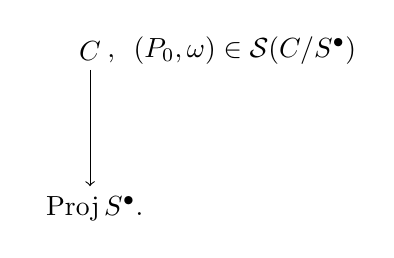
\begin{tikzpicture}
         \node (T)  at (0, 2) {$C$}; 
         \node (RT) at (1.8, 2) {$\text{,} ~~ (P_0,\omega) \in \CS(C/\s)$}; 
         \node (B)  at (0, 0) {$~\Proj \s \text{.}$}; 
         \draw [->] (T) -- (B); 
 \end{tikzpicture}
 \end{center}
\end{prop}
\begin{proof}
 Let $E/S/\BZ[1/4]$ be an elliptic curve with $(Q,\eta) \in \CS(E/S)$, 
 locally on $\Spec R \subset S$ given by the Weierstrass equation 
 \[
  y^2 + a_1 x y + a_3 y = x^3 + a_2 x^2 + a_4 x + a_6 
 \]
 with $Q = (x_0,y_0)$.  We need only show that there is a unique 
 $R$-isomorphism from $E$ to $C \otimes_{\s} R$ which sends $(Q,\eta)$ 
 to $(P_0,\omega)$, where the map $\s \to R$ in $C \otimes_{\s} R$ is 
 given by $a \mapsto a_1'$ and $b \mapsto a_2'$ for some $a_1'$, 
 $a_2' \in R$ uniquely determined below.  

 Recall from Section \ref{subsec:gp} that the only change of variables 
 fixing the identity and preserving the form of a Weierstrass equation 
 is 
 \begin{equation}
 \label{change}
  x = u^2 x' + r \qquad \ad \qquad y = u^3 y' + u^2 s x' + t 
 \end{equation}
 where $r$, $s$, $t \in R$ and $u \in R^\times$.  We make a sequence of 
 changes of variables, where $x'$ and $y'$ are the variables after each 
 change satisfying a Weierstrass equation with adjusted coefficients 
 (cf.~Example \ref{ex:velu}): 
 \begin{itemize}
  \item set 
  \[
   x = x' + x_0 \qquad \ad \qquad y = y' + y_0 \qquad \qquad \quad ~~~
  \]
  which sends $Q$ to $P_0 = (0,0)$, and $x'$ and $y'$ satisfy 
  \[
   y^2 + a_1 x y + a_3 y = x^3 + a_2 x^2 + a_4 x 
  \]
  with 
  \[
   \dot{y}(0,0) \ce \frac{dy}{dx}(0,0) = \frac{a_4}{a_3} 
  \]
  (the fact that $Q$ has exact order 4 forces $a_3$ to be invertible); 

  \item set 
  \[
   x = x' \qquad \ad \qquad y = y' + \frac{a_4}{a_3} \cdot x \qquad ~
  \]
  which fixes $P_0$ and makes $\dot{y}(0,0) = 0$, and $x'$ and $y'$ 
  satisfy 
  \[
   y^2 + a_1 x y + a_3 y = x^3 + a_2 x^2 
  \]
  with $(-a_2,0) = 2 P_0$ a 2-torsion point so that $a_3 = a_1 a_2$ (we 
  have formally $\dot{y}(-a_2,0) = a_2^2 / (a_3 - a_1 a_2)$); 

  \item set 
  \[
   x = u^2 x' \qquad \ad \qquad y = u^3 y' \qquad \qquad \quad ~~~
  \]
  for some $u \in R^\times$ to scale the image of $\eta$ under the 
  previous changes of variables into $\omega$.  
 \end{itemize}
 These steps exhaust the coefficients in \eqref{change} and give a 
 unique $R$-isomorphism from $E$ to an elliptic curve with Weierstrass 
 equation 
 \[
  y^2 + a_1' x y + a_1' a_2' y = x^3 + a_2' x^2 
 \]
 for some $a_1'$, $a_2' \in R$.  This is $C/\s$ along the base change 
 \begin{equation*}
 \begin{split}
      \s \longrightarrow & ~ R \\
  a ~ \mapsto \thinspace & ~ a_1' \\
  b ~ \mapsto \thinspace & ~ a_2'.  
 \end{split}
 \end{equation*}
\end{proof}

From Proposition \ref{prop:C} above, we see that $\CM(\CS) = \Proj \s$ 
where 
\[
 \s = \BZ[1/4][a,b,\Delta^{-1}] 
\]
with $|a| = 1$, $|b| = 2$, and $\Delta = a^2 b^4 (a^2 -16 b)$.  To work 
with this moduli scheme, we consider the weighted projective space 
\[
 \Proj \BZ[1/4][a,b].  
\]
For every element $f$ homogeneous of positive degree in $\BZ[1/4][a,b]$, 
there is a distinguished open subset 
\[
 \Proj \BZ[1/4][a,b][f^{-1}] 
 \cong \Spec \big( \BZ[1/4][a,b][f^{-1}] \big)^0.  
\]
In particular, taking $f = \Delta$, we see that $\CM(\CS)$ is an affine 
open subscheme of the weighted projective space $\Proj \BZ[1/4][a,b]$.  
Moreover, in the \'etale topology, this weighted projective space is 
covered by two affine coordinate charts: the first one is 
\[
 \Proj \BZ[1/4][a,b][a^{-1}] 
 \cong \Spec \BZ[1/4] \! \left[ \frac{b}{a^2} \right], 
\]
which is open and contains $\CM(\CS)$ (inverting $\Delta$ automatically 
inverts $a$); the second one is 
\[
 \Proj \BZ[1/4][a,b][u^{-1}] 
 \cong \Spec \BZ[1/4] \! \left[ \frac{a}{u} \right], ~
\]
with $u$ an adjoined element such that $u^2 = b$, which is finite 
\'etale with Galois group $\{\pm1\}$ (2 is invertible on 
$\Proj \BZ[1/4][a,b]$).  Both coordinate charts contain the 
supersingular locus at the prime 3 which we identified in Example 
\ref{ex:H} as a single closed point 
\[
 \Proj \s / (3,H) \cong \Spec \BF_3 
\]
where $H = a^2 + b$.  We summarize the above in a diagram.  
\begin{equation}
\label{chart}
 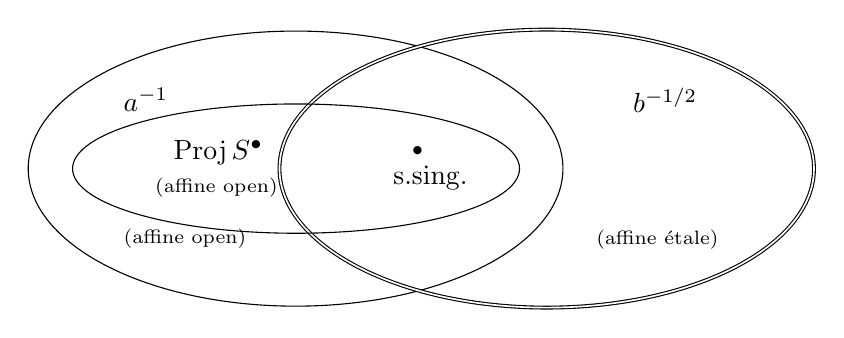
\begin{tikzpicture}[baseline=(current bounding box.center), every fit/.style={ellipse,draw,inner sep=0pt}, mytext/.style={inner sep=6pt}]
         \node[mytext,align=left,rectangle] (a) at (0, 0) {$a^{-1}$ \\ \\ \\ \\ $\scriptstyle \text{(affine open)}$}; 
         \node[mytext,align=left,rectangle] (b) at (6, 0) {$\quad~ b^{-1/2}$ \\ \\ \\ \\ $\scriptstyle \text{(affine \'etale)}$}; 
         \node[mytext,align=left,rectangle] (c) at (3, 0) {$\quad~ _\bullet$ \\ ~ s.sing.}; 
         \node[mytext,align=left,rectangle] (c') at (3.2, 0) {}; 
         \node[mytext,align=left,rectangle] (d) at (.4, 0) {$~~ \Proj \s$ \\ $\scriptstyle \text{(affine open)}$}; 
         \node[draw,fit=(a) (c)] {}; 
         \node[draw,double,fit=(b) (c)] {}; 
         \node[draw,fit=(d) (c')] {}; 
 \end{tikzpicture}
\end{equation}

In view of Proposition \ref{prop:C}, $C/\s$ is a universal deformation 
of the supersingular elliptic curve $C_0/\BF_3$ (see \eqref{C_0}).  
Recall from Section \ref{subsec:E} that the formal group associated to a 
Morava $E$-theory is the universal deformation of a formal group over a 
perfect field to the corresponding Lubin-Tate ring.  We can now produce 
a Morava $E$-theory spectrum from the above universal deformation of a 
supersingular elliptic curve via the Serre-Tate theorem (Theorem 
\ref{thm:serretate}).  

\begin{ex}
\label{ex:E}
 We follow the convention that elements in algebraic degree $n$ lie in 
 topological degree $2n$, and work in the affine \'etale coordinate 
 chart ``$b^{-1/2}$'' in \eqref{chart}.  Write $c \ce a/u$ so that 
 \[
  a = u c \qquad \ad \qquad b = u^2.  
 \]
 Consider the graded ring 
 \[
  \s[u^{-1}] \cong \BZ [1/4] [a, \Delta^{-1}] [u^{\pm1}] 
 \]
 where $|u| = 1$, and write 
 \[
  S \ce \big( \s[u^{-1}] \big)^0 \cong \BZ [1/4] [c, \delta^{-1}] 
 \]
 where $\delta = u^{-12} \Delta = c^2 (c^2 - 16)$.  Thus $\Spec S$ is 
 the restriction of $\CM(\CS)$ to this affine \'etale coordinate chart.  

 Write 
 \[
  \HS \ce \BZ_9 \llbracket h \rrbracket 
 \]
 where 
 \begin{equation}
 \label{h}
  h \ce u^{-2} H = c^2 + 1.  
 \end{equation}
 Let $i$ be an element generating $\BZ_9$ over $\BZ_3$ with $i^2 = -1$.  
 We may choose 
 \[
  c \equiv i \md (3,h) 
 \]
 and we have 
 \[
  \delta \equiv -1 \md (3,h) 
 \]
 where $(3,h)$ is the maximal ideal of the complete local ring $\HS$.  
 Then by Hensel's lemma, both $c$ and $\delta$ lie in $\HS$, and both 
 are invertible.  Thus 
 \[
  \HS \cong S_{(3,h)}^\wedge.  
 \]

 Now $C$ restricts to $S$ as 
 \begin{equation}
 \label{Cc}
  y^2 + c x y + c y = x^3 + x^2, 
 \end{equation}
 and $\HC$ is a formal group over $\HS$.  In view of \eqref{h} and 
 \eqref{H}, its reduction to $\HS / (3,h) \cong \BF_9$ is $\HC_0$, which 
 is a formal group of height 2.  By Theorem \ref{thm:serretate} and 
 Proposition \ref{prop:C}, $C[3^\infty]$ is the universal deformation of 
 $C_0[3^\infty]$ as 3-divisible groups.  Since $\HT(\HC_0) = 2$, 
 $C_0[3^\infty]$ is all formal (see Section \ref{subsec:fg}), i.e., 
 \[
  C_0[3^\infty] = \big( C_0[3^\infty] \big)^0 \cong \HC_0.  
 \]
 Thus $\HC \cong \big( C[3^\infty] \big)^0$ is the universal deformation 
 of $\HC_0$ as formal groups.  Let $E$ be the Morava $E$-theory spectrum 
 associated to $\HC_0/\BF_9$.  Then 
 \[
  E_* \cong \BZ_9 \llbracket h \rrbracket [u^{\pm 1}] 
 \]
 where $u$ is in topological degree 2, and it corresponds to a local 
 uniformizer at the identity of $C$.  
\end{ex}

\begin{rmk}
\label{rmk:rep}
 In view of \eqref{action}, $[\omega]$ is a $\BG_m$-torsor over $\Ell$, 
 and the induced action of $\BG_m$ on $C/\s$ fixes 
 $P_0(0,0) \in [\G_1(4)](C/\s)$.  Thus over $\Ell/\BZ[1/4]$ we have 
 \[
  \CM \big( [\G_1(4)] \big) 
  \cong \CM \big( [\G_1(4)], [\omega] \big) \big/ \BG_m 
 \]
 (cf.~\cite[7.1.3]{KM} and \cite[Theorem 1.10]{GIT}).  As 
 $S = \big( \s[u^{-1}] \big)^0$ consists of the $\BG_m$-invariants of 
 $\s[u^{-1}]$, locally over $\CM \big( [\G_1(4)] \big)$ the universal 
 elliptic curve with a $\G_1(4)$-structure is then given by \eqref{Cc}.  
\end{rmk}

\subsubsection*{The moduli problem $[\G_0(3)]$}

We denote by 
\[
 \CS_3 \ce \big( [\G_0(3)], \CS \big) \quad \text{over} \quad 
 \Ell/\BZ[1/4] 
\]
the simultaneous moduli problem which carries the data of a cyclic 
subgroup of degree 3 (cf.~Definition 
\ref{def:level}\thinspace \eqref{level(iv)}) together with the data of 
$\CS$ (see \eqref{CS}) on each elliptic curve over a $\BZ[1/4]$-scheme.  
It is representable, as $[\G_0(3)]$ is relatively representable and 
$\CS$ is representable (see Theorem \ref{thm:relrep} and Proposition 
\ref{prop:C}).  

Recall from \isog{i} that we constructed the universal degree-3 isogeny 
$\psi$ with source $C$ over the graded ring $\s_3$.  In view of 
\cite[6.8.7]{KM} we then have 
\[
 \CM(\CS_3) \cong [\G_0(3)]_{C/\s} \cong \Proj \s_3.  
\]
As $\s_3 = \s [\K] \big/ \big( W(\K) \big)$ is an $\s$-module of rank 4, 
$\Proj \s_3$ is affine and is covered by two affine coordinate charts 
which are extensions of those in \eqref{chart}.  

\begin{ex}
\label{ex:M(S_3)}
 Notations as in Example \ref{ex:E}, the restriction of this moduli 
 scheme $\CM(\CS_3)$ to the affine \'etale coordinate chart 
 ``$b^{-1/2}$'' is $\Spec S_3$ where 
 \begin{equation}
 \label{S_3}
  S_3 \ce S [\A] \big/ \big( w(\A) \big) 
 \end{equation}
 with 
 \[
  w(\A) = \A^4 - 6 \A^2 + (c^2 - 8) \A - 3.  
 \]
 In particular, we have 
 \[
  [\G_0(3)]_{\HC/\thinspace\HS} 
  \cong \Spec \BZ_9 \llbracket h, \A \rrbracket \big/ 
  \big( \A^4 - 6 \A^2 + (h - 9) \A - 3 \big), 
 \]
 which exhibits the moduli problem $[\G_0(3)]$ as an {\em open 
 arithmetic surface} with two parameters $h$ and $\A$ (we have 
 $3 = \A^4 - 6 \A^2 + (h - 9) \A$).  More precisely, we have seen in 
 Example \ref{ex:E} that $\HC / \BZ_9 \llbracket h \rrbracket$ is the 
 universal formal deformation of the supersingular elliptic curve 
 $C_0/\BF_9$ with $u$ a local uniformizer.  The first parameter 
 $h = H(C/S,\omega)$ (see \eqref{h} and \eqref{H}) arises as a parameter 
 for this deformation (cf.~\cite[12.4.4]{KM}).  We have seen in Remark 
 \ref{rmk:K} that 
 \[
  \K = u(Q) \cdot u(-Q) 
 \]
 where $Q$ is a nonzero 3-torsion point on $C$ generating the universal 
 degree-3 subgroup $G$.  Thus, as the restriction of $\K$ over $S_3$, 
 the second parameter $\A$ arises as the norm 
 \[
  N \big( u(Q) \big) \ce \prod_{\sigma \in \Aut(G)} u(\sigma \cdot Q).  
 \]

 There is a second parametrization for $[\G_0(3)]$ given by $\A$ and 
 $\A'$ where $\A'$ is the restriction of $\K'$ over $S_3$ (see Corollary 
 \ref{cor:K'}).  We have 
 \[
  [\G_0(3)]_{\HC/\thinspace\HS} 
  \cong \Spec \BZ_9 \llbracket \A, \A' \rrbracket / (\A \A' + 3) 
 \]
 and 
 \[
  \A' = -h - \A^3 + 6 \A + 9.  
 \]

 These are examples of the two parametrizations for $[\G_0(p^n)]$ listed 
 in \cite[7.7]{KM}.  
\end{ex}

\begin{rmk}
 Another viewpoint for the moduli scheme $\CM(\CS_3)$ is that 
 \eqref{S_3} exhibits the moduli problem $\CS_3$ as a {\em relative 
 curve over $\Spec \BZ$}.  Its {\em compactification} 
 $\overline{\CM}(\CS_3)[1/6]$ is a proper smooth curve over $\BZ[1/6]$ 
 with geometrically connected fibers, in which the {\em scheme of cusps} 
 is finite \'etale over $\BZ[1/6]$ (see \cite[8.6 and 10.9.5]{KM}).  
 This is an example of the moduli problem 
 $\big( [\G_1(N_1)], [\G_0(N_2)] \big)$, with $N_1$ and $N_2$ relatively 
 prime and $N_1 \geq 4$, listed in \cite[10.9.6]{KM}.  
\end{rmk}

\subsubsection*{Abstract endomorphisms of $[\G_1(4)]$ and $[\G_0(3)]$}

Recall from Definition \ref{def:abstract} that an abstract morphism 
$\CP \to \CP'$ of moduli problems sends each pair 
$\big( E/S, ~ x \in \CP(E/S) \big)$ to 
$\big( E'/S, ~ x' \in \CP'(E'/S) \big)$.  The constructions in 
Propositions \ref{prop:isog} and \ref{prop:frob^2} each gives rise to an 
example of an abstract endomorphism.  

\begin{ex}
\label{ex:ab4}
 We continue with the notations in Example \ref{ex:M(S_3)} and work in 
 the affine \'etale coordinate chart ``$b^{-1/2}$.''  By \isog{i}, in 
 $xy$-coordinates, $C'$ restricts to $S_3$ as 
 \[
  y^2 + c' x y + c' y = x^3 + x^2 
 \]
 where 
 \[
  c' = \frac{1}{c} \big( (c^2 - 4) \A^3 + 4 \A^2 + (-6 c^2 + 20) \A 
  + c^4 - 12 c^2 + 12 \big).  
 \]
 Since this equation is in the form of \eqref{Cc}, the isogeny $\psi$ 
 determines an assignment 
 \begin{equation}
 \label{assign}
  \big( C/S_3, ~~ P_0(0,0) \in [\G_1(4)](C/S_3) \big) \longmapsto 
  \big( C'/S_3, ~~ P_0(0,0) \in [\G_1(4)](C'/S_3) \big).  
 \end{equation}
 By Proposition \ref{prop:C} and Remark \ref{rmk:rep}, over the affine 
 \'etale coordinate chart ``$b^{-1/2}$,'' we have a universal pair 
 \[
  \big( C/S, ~~ P_0(0,0) \in [\G_1(4)](C/S) \big) 
 \]
 for the moduli problem $[\G_1(4)]$ over $\Ell/\BZ[1/4]$.  However, in 
 \eqref{assign}, $S_3$ is an extension of $S$, and $C'$ is not defined 
 over $S$.  To get an abstract endomorphism of $[\G_1(4)]$, we consider 
 its restriction over $\BF_9$ to a formal neighborhood of the 
 supersingular locus, where we have $\A = 0$ (cf.~\eqref{Kmod3}).  The 
 above assignment then sends 
 \[
  C \co y^2 + c x y + c y = x^3 + x^2, \qquad ~~~ P_0(0,0) 
 \]
 to 
 \[
  \thinspace C' \co y^2 + c^3 x y + c^3 y = x^3 + x^2, \qquad P_0(0,0).  
 \]
 In particular, under this further restriction, locally we have an 
 induced endomorphism of the moduli scheme 
 $\CM([\G_1(4)]) \cong \Spec S$ which sends $c$ to $c^3$.  
\end{ex}

\begin{rmk}
 In contrast, over the affine open coordinate chart ``$a^{-1}$,'' 
 although the assignment analogous to \eqref{assign} locally induces an 
 endomorphism of the moduli scheme near the supersingular locus, it does 
 not lift to an assignment {\em within} the chart.  Precisely, if we 
 denote by $\Tc$ and $\TA$ the analogs of $c$ and $\A$ respectively, we 
 have 
 \[
  C \co y^2 + x y + \Tc y = x^3 + \Tc x^2 
 \]
 and 
 \[
  \quad ~~ C' \co y^2 + r x y + r \Tc^3 y = x^3 + \Tc^3 x^2 
 \]
 where 
 \begin{equation*}
 \begin{split}
   r = & ~ (-4 \Tc^5 + \Tc^4) \TA^3 + 4 \Tc^4 \TA^2 + (20 \Tc^3 - 6 \Tc^2) \TA + 12 \Tc^2 - 12 \Tc + 1 \\
  \neq & ~ 1.  
 \end{split}
 \end{equation*}
 This makes the chart less convenient for the purpose of studying power 
 operations (cf.~the proof of Corollary \ref{cor:psi3} below), 
 particularly their compositions.  
\end{rmk}

\begin{ex}
\label{ex:ab3}
 In \cite[11.3.1]{KM} (cf.~\cite[Lemmas 7-10]{atkinlehner}), for every 
 integer $m \geq 1$, the {\em involution $W_m$ of $[\G_0(m)]$} is 
 defined as an abstract endomorphism of $[\G_0(m)]$ which sends 
 \[
  (E/S, ~~ \text{~cyclic subgroup~} G \text{~of degree~} m) \quad 
  \text{to} \quad \big( E'/S \ce (E/G)/S, ~~ G' \ce E[m]/G \big) 
 \]
 (the subgroup $G'$ is cyclic of degree $m$ by Theorem \ref{thm:tors} 
 and \cite[12.2.5]{KM}).  

 By construction of $\psi'$ in Proposition \ref{prop:frob^2}, locally 
 over the affine \'etale coordinate chart ``$b^{-1/2}$,'' we have an 
 involution of the moduli problem $\big( [\G_0(3)], [\G_1(4)] \big)$ 
 which sends 
 \[
  \qquad (C/S_3, ~~ \psi, ~~ P_0) \qquad \text{to} \qquad 
  (C'/S_3, ~~ \psi', ~~ P_0).  
 \]
 In particular, by \isog{i} and Corollary \ref{cor:K'}, the induced 
 endomorphism $t$ of the moduli scheme $\Spec S_3$ is given by 
 \begin{equation*}
 \begin{split}
   c \longmapsto & ~ \frac{1}{c} \big( (c^2 - 4) \A^3 + 4 \A^2 + (-6 c^2 + 20) \A + c^4 - 12 c^2 + 12 \big), \\
  \A \longmapsto & ~ -\A^3 + 6 \A - c^2 + 8, 
 \end{split}
 \end{equation*}
 and we have $t \circ t = \id$ (cf.~\cite[Section 5]{tmf3}).  
\end{ex}


\section{An example of the power operation structure on an elliptic cohomology theory}
\label{sec:p3}

\subsection{Summary of the main example in Section \ref{sec:ec}}
\label{subsec:summary}

Recall from Section \ref{subsec:E} that a Morava $E$-theory of height 2 
at the prime 3 has its formal group as the universal deformation of a 
height-2 formal group over a perfect field of characteristic 3.  In 
Example \ref{ex:E} we produced such an $E$-theory spectrum from a 
universal deformation of a supersingular elliptic curve over $\BF_9$.  

\begin{prop}[cf.~Proposition \ref{prop:C} and Remark \ref{rmk:rep}]
 Over $\BZ[1/4]$, the moduli problem of elliptic curves with a choice of 
 a point of exact order 4 is representable.  Locally for the \'etale 
 topology on the moduli scheme, the universal elliptic curve is given by 
 \begin{equation}
 \label{C}
  C \co y^2 + c x y + c y = x^3 + x^2, 
 \end{equation}
 with chosen point $(0,0)$, over the ring 
 \[
  S = \BZ[1/4][c,\delta^{-1}] 
 \]
 where $\delta = c^2 (c^2 - 16)$.  
\end{prop}

Let $C_0$ be the restriction of $C$ to the supersingular locus 
\[
 \Spec \BF_9 \cong \Spec S/(3,h) 
\]
where $h = c^2 + 1$ (see Examples \ref{ex:H} and \ref{ex:E}).  The 
Morava $E$-theory spectrum $E$ associated to $\HC_0/\BF_9$ has homotopy 
groups 
\[
 E_* \cong \BZ_9 \llbracket h \rrbracket [u^{\pm1}] 
\]
where $|h| = 0$ and $|u| = 2$.  In particular, 
\begin{equation}
\label{E0}
 E_0 \cong \BZ_9 \llbracket h \rrbracket \cong S_{(3,h)}^\wedge.  
\end{equation}

In Section \ref{subsec:isog} we first constructed a deformation of 
Frobenius from the following.  

\begin{prop}[cf.~Proposition \ref{prop:isog} and Example \ref{ex:ab4}]
\label{prop:df}
 \mbox{}
 \begin{enumerate}[(i)]
  \item \label{df(i)} The universal degree-3 isogeny $\psi$ with source 
  $C$ is defined over the ring 
  \begin{equation}
  \label{S3}
   S_3 = S [\A] \big/ \big( w(\A) \big) 
  \end{equation}
  where 
  \[
   w(\A) = \A^4 - 6 \A^2 + (c^2 - 8) \A - 3, 
  \]
  and has target the elliptic curve 
  \begin{equation}
  \label{C'}
   C' \co y^2 + c' x y + c' y = x^3 + x^2 
  \end{equation}
  where 
  \[
   c' = \frac{1}{c} \big( (c^2 - 4) \A^3 + 4 \A^2 + (-6 c^2 + 20) \A 
   + c^4 - 12 c^2 + 12 \big).  
  \]

  \item The kernel $G$ of $\psi$ is generated by a point $Q$ of exact 
  order 3 with coordinates $(d,e)$ satisfying 
  \begin{equation}
  \label{A}
  \begin{split}
   \A = & -\frac{1}{c^2 - 16} \big( c d^7 + (3 c^2 - 2) d^6 + (3 c^3 - 6 c) d^5 + (c^4 + c^2 + 2) d^4 \\
        & + (4 c^3 - 15 c) d^3 + (c^2 + 2) d^2 - 12 c d - 18 \big) \\
      = & ~ c e - d^2.  
  \end{split}
  \end{equation}

  \item The restriction of $\psi$ to the supersingular locus at the 
  prime 3 is the 3-power Frobenius endomorphism.  

  \item The induced map $\psi^*$ on the relative cotangent space of $C'$ 
  at the identity sends $du$ to $\A du$.  
 \end{enumerate}
\end{prop}

We then constructed a composite of deformations of Frobenius from the 
following.  

\begin{prop}[cf.~Proposition \ref{prop:frob^2}, Corollary \ref{cor:K'}, and Example \ref{ex:ab3}]
\label{prop:df^2}
 Notations as in the above proposition, let 
 \[
  \psi' \co C' \longrightarrow C'/G' 
 \]
 be the degree-3 isogeny over $S_3$ with kernel $G' = C[3]/G$.  Then the 
 following diagram of elliptic curves over $S_3$ commutes: 
 \begin{equation}
 \label{df^2}
  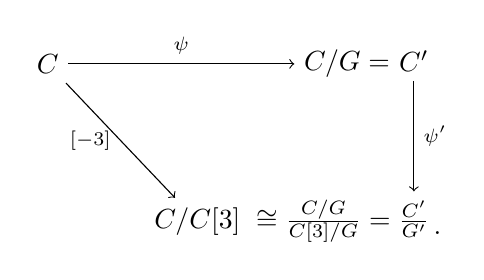
\begin{tikzpicture}[baseline=(current bounding box.center)]
          \node (LT) at (0, 2) {$C$}; 
          \node (MT) at (3.8, 2) {$C/G = $}; 
          \node (RT) at (4.65, 2.04) {$C'$}; 
          \node (LB) at (1.9, 0) {$C/C[3]$}; 
          \node (MB) at (3.5, 0) {$\cong \frac{C/G}{C[3]/G} = $}; 
          \node (RB) at (4.65, 0.025) {$\frac{C'}{G'}$}; 
          \node at (4.95, -0.15) {.}; 
          \draw [->] (LT) -- node [above] {$\scriptstyle \psi$} (MT); 
          \draw [->] (LT) -- node [left] {$\scriptstyle [-3]$} (LB); 
          \draw [->] (RT) -- node [right] {$\scriptstyle \psi'$} (RB); 
  \end{tikzpicture}
 \end{equation}
 Moreover the isogenies in this diagram induce maps on relative 
 cotangent spaces at the identity, and we have a commutative diagram 
 \begin{center}
 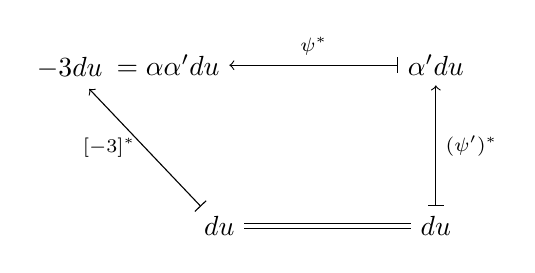
\begin{tikzpicture}
         \node (LT) at (0, 2) {$-3 du$}; 
         \node (MT) at (1.25, 2.04) {$= \A \A' du$}; 
         \node (RT) at (4.65, 2.04) {$\A' du$}; 
         \node (LB) at (1.9, 0) {$du$}; 
         \node (RB) at (4.65, 0) {$du$}; 
         \draw [|->] (RT) -- node [above] {$\scriptstyle \psi^*$} (MT); 
         \draw [|->] (LB) -- node [left] {$\scriptstyle [-3]^*$} (LT); 
         \draw [|->] (RB) -- node [right] {$\scriptstyle (\psi')^*$} (RT); 
         \draw [double distance=1.3pt] (LB) -- (RB); 
 \end{tikzpicture}
 \end{center}
 where 
 \begin{equation}
 \label{A'}
  \A' = -\A^3 + 6 \A - c^2 + 8.  
 \end{equation}
\end{prop}

In the next section, via the bridge of Theorem \ref{thm:bridge} between 
deformations of Frobenius and power operations, we will compute power 
operations for the Morava $E$-theory $E$ from Propositions \ref{prop:df} 
and \ref{prop:df^2} above.  


\subsection{$K(2)$-local power operations}
\label{subsec:K(2)po}

\subsubsection*{Total power operations}

Recall from Section \ref{subsec:arise} (cf.~\eqref{total}) that there is 
an additive total power operation 
\[
 \p \co E^0 \longrightarrow E^0 B\Sigma_3 / I 
\]
where 
\[
 I = \bigoplus_{0<i<3} {\rm image} 
 \big( E^0 B(\Sigma_i \times \Sigma_{3-i}) 
 \xrightarrow{\rm transfer} E^0 B\Sigma_3 \big).  
\]
The source of $\p$ is 
\[
 E^0 \cong \BZ_9 \llbracket h \rrbracket \cong S_{(3,h)}^\wedge 
\]
(cf.~\eqref{E0}) in which $c$ and $i$ are elements with $c^2 + 1 = h$ 
and $i^2 = -1$.  The target of $\p$ is 
\begin{equation}
\label{strickland}
 E^0 B\Sigma_3 / I \cong \big( S_3 \big)_{(3,h)}^\wedge 
\end{equation}
by Strickland's computation of Morava $E$-theory of symmetric groups 
(cf.~\cite[Theorem 1.1]{Str98}).  In view of \eqref{S3} we then have 
\begin{equation}
\label{strickland'}
 E^0 B\Sigma_3 / I \cong E^0 [\A] \big/ \big( w(\A) \big).  
\end{equation}

\begin{cor}
\label{cor:psi3}
 The total power operation 
 \[
  \p \co E^0 \longrightarrow E^0 B\Sigma_3 / I 
  \cong E^0 [\A] \big/ \big( w(\A) \big) 
 \]
 is given by 
 \begin{equation*}
 \begin{split}
  \p(h) = & ~ h^3 + (\A^3 - 6 \A - 27) h^2 + 3 (-6 \A^3 + \A^2 + 36 \A + 67) h \\
          & + 57 \A^3 - 27 \A^2 - 334 \A - 342, \\
  \p(c) = & ~ c^3 + (\A^3 - 6 \A - 12) c - 4 (\A + 1)^2 (\A - 3) c^{-1}, \\
  \p(i) \thinspace = & -i, 
 \end{split}
 \end{equation*}
 where 
 \begin{equation}
 \label{Amod3}
  \A \equiv 0 \md 3.  
 \end{equation}
\end{cor}
\begin{proof}
 By Theorem \ref{thm:bridge} there is a correspondence between the 
 universal degree-3 isogeny $\psi$ over $S_3$, which is a deformation of 
 Frobenius, and the total power operation $\p$.  In particular, in view 
 of \eqref{C} and \eqref{C'}, $\p(c)$ is given by $c'$.  As $\p$ is a 
 ring homomorphism, we then get the formula for $\p(h) = \p(c^2 + 1)$.  
 We also have 
 \[
  \big( \p(i) \big)^2 = \p(-1) = -1 
 \]
 which implies $\p(i) = i$ or $-i$.  We exclude the former possibility 
 in view of the Frobenius congruence 
 \[
  \p(i) \equiv i^3 \md 3 
 \]
 (see Definition \ref{def:alg} and \eqref{frobcong}).  The congruence 
 \eqref{Amod3} follows from \eqref{dmod3} and \eqref{A} 
 (cf.~\eqref{Kmod3}).  
\end{proof}

More generally, let $A$ be a $K(2)$-local commutative $E$-algebra.  
From Corollary \ref{cor:psi3} we have a total power operation 
\[
 \p \co A_0 \longrightarrow A_0 \otimes_{E_0} (E^0 B\Sigma_3 / I) 
 \cong A_0 [\A] \big/ \big( w(\A) \big).  
\]
We also have a composite of total power operations 
\begin{equation}
\label{psi3^2}
\begin{split}
 A_0 \stackrel{\p}{\longrightarrow} A_0 \otimes_{E_0} (E^0 B\Sigma_3 / I) \stackrel{\p}{\longrightarrow} 
 & ~ \big( A_0 \otimes_{E_0} (E^0 B\Sigma_3 / I) \big) \tensor[^\p]{\otimes}{_{E_0 [\A]}} (E^0 B\Sigma_3 / I) \\
 \cong \thinspace \thinspace & ~ \Big( A_0 [\A] \big/ \big( w(\A) \big) \Big) \tensor[^\p]{\otimes}{_{E_0 [\A]}} \Big( E^0 [\A] \big/ \big( w(\A) \big) \Big) 
\end{split}
\end{equation}
where the elements in the target $M \tensor[^\p]{\otimes}{_R} N$ are 
subject to the equivalence relation 
\[
 m \otimes (r \cdot n) \sim \big( m \cdot \p(r) \big) \otimes n 
\]
for $m \in M$, $n \in N$, and $r \in R$, with 
\[
 \p(\A) = -\A^3 + 6 \A - h + 9 
\]
by \eqref{A'}, as well as other relations in a usual tensor product.  

\subsubsection*{Individual power operations}

Recall from Section \ref{subsec:arise} (cf.~\eqref{individual}) that for 
each $\A \in \pi_0 \BP_E^3(E) \cong E_0 B\Sigma_3$ there is an 
individual power operation $Q_\A$ given by pairing with $\A$ the total 
power operation $P^3$.  In view of \eqref{strickland'} we have additive 
individual power operations from the total power operation $\p$ as 
follows.  

\begin{defn}
\label{def:Q}
 Let $A$ be a $K(2)$-local commutative $E$-algebra.  Define the 
 individual power operations 
 \[
  Q_k \co A_0 \longrightarrow A_0 
 \]
 for $k = 0$, 1, 2, and 3 by 
 \[
  \p (x) = Q_0(x) + Q_1(x) \A + Q_2(x) \A^2 + Q_3(x) \A^3.  
 \]
\end{defn}

\begin{prop}
\label{prop:Q}
 The following relations hold among the individual power operations 
 $Q_0$, $Q_1$, $Q_2$, and $Q_3$: 
 \begin{enumerate}[(i)]
  \item \label{Q(i)} $Q_0(1) = 1, \quad Q_1(1) = Q_2(1) = Q_3(1) = 0;$ 

  \item \label{Q(ii)} $Q_k(x+y) = Q_k(x) + Q_k(y) \text{~for all~} k;$ 

  \item \label{Q(iii)} {\em Commutation relations }
  \begin{equation*}
  \begin{split}
   Q_0(h x) = & ~ (h^3 - 27 h^2 + 201 h - 342) Q_0(x) + (3 h^2 - 54 h + 171) Q_1(x) \qquad \qquad \\
              & + (9 h - 81) Q_2(x) + 24 Q_3(x), \\
   Q_1(h x) = & ~ (-6 h^2 + 108 h - 334) Q_0(x) + (-18 h + 171) Q_1(x) + (-72) Q_2(x) \\
              & + (h - 9) Q_3(x), \\
   Q_2(h x) = & ~ (3 h - 27) Q_0(x) + 8 Q_1(x) + 9 Q_2(x) + (-24) Q_3(x), \\
   Q_3(h x) = & ~ (h^2 - 18 h + 57) Q_0(x) + (3 h - 27) Q_1(x) + 8 Q_2(x) + 9 Q_3(x), \\
   Q_0(c x) = & ~ (c^3 - 12 c + 12 c^{-1}) Q_0(x) + (3 c - 12 c^{-1}) Q_1(x) + (12 c^{-1}) Q_2(x) \\
              & + (-12 c^{-1}) Q_3(x), \\
   Q_1(c x) = & ~ (-6 c + 20 c^{-1}) Q_0(x) + (-20 c^{-1}) Q_1(x) + (- c + 20 c^{-1}) Q_2(x) \\
              & + (4 c - 20 c^{-1}) Q_3(x), \\
   Q_2(c x) = & ~ (4 c^{-1}) Q_0(x) + (-4 c^{-1}) Q_1(x) + (4 c^{-1}) Q_2(x) + (- c - 4 c^{-1}) Q_3(x), \\
   Q_3(c x) = & ~ (c - 4 c^{-1}) Q_0(x) + (4 c^{-1}) Q_1(x) + (-4 c^{-1}) Q_2(x) + (4 c^{-1}) Q_3(x), \\
   Q_k(i x) = & ~ (-i) Q_k(x) \text{~for all~} k; 
  \end{split}
  \end{equation*}

  \item \label{Q(iv)} {\em Adem relations }
  \begin{equation*}
  \begin{split}
   Q_1Q_0(x) = & ~ (-6) Q_0Q_1(x) + 3 Q_2Q_1(x) + (6 h - 54) Q_0Q_2(x) + 18 Q_1Q_2(x) \\
               & + (-9) Q_3Q_2(x) + (-6 h^2 + 108 h - 369) Q_0Q_3(x) \\
               & + (-18 h + 162) Q_1Q_3(x) + (-54) Q_2Q_3(x), \\
   Q_2Q_0(x) = & ~ 3 Q_3Q_1(x) + (-3) Q_0Q_2(x) + (3 h - 27) Q_0Q_3(x) + 9 Q_1Q_3(x), \\
   Q_3Q_0(x) = & ~ Q_0Q_1(x) + (-h + 9) Q_0Q_2(x) + (-3) Q_1Q_2(x) \\
               & + (h^2 - 18 h + 63) Q_0Q_3(x) + (3 h - 27) Q_1Q_3(x) + 9 Q_2Q_3(x); \qquad \qquad
  \end{split}
  \end{equation*}

  \item \label{Q(v)} {\em Cartan formulas }
  \begin{equation*}
  \begin{split}
   Q_0(xy) = & ~ Q_0(x) Q_0(y) + 3 \big( Q_3(x) Q_1(y) + Q_2(x) Q_2(y) + Q_1(x) Q_3(y) \big) \\
             & + 18 Q_3(x) Q_3(y), \\
   Q_1(xy) = & ~ \big( Q_1(x) Q_0(y) + Q_0(x) Q_1(y) \big) \\
             & + (-h + 9) \big( Q_3(x) Q_1(y) + Q_2(x) Q_2(y) + Q_1(x) Q_3(y) \big) \\
             & + 3 \big( Q_3(x) Q_2(y) + Q_2(x) Q_3(y) \big) + (-6 h + 54) Q_3(x) Q_3(y), \\
   Q_2(xy) = & ~ \big( Q_2(x) Q_0(y) + Q_1(x) Q_1(y) + Q_0(x) Q_2(y) \big) \\
             & + 6 \big( Q_3(x) Q_1(y) + Q_2(x) Q_2(y) + Q_1(x) Q_3(y) \big) \\
             & + (-h + 9) \big( Q_3(x) Q_2(y) + Q_2(x) Q_3(y) \big) + 39 Q_3(x) Q_3(y), \\
   Q_3(xy) = & ~ \big( Q_3(x) Q_0(y) + Q_2(x) Q_1(y) + Q_1(x) Q_2(y) + Q_0(x) Q_3(y) \big) \qquad \qquad \qquad \\
             & + 6 \big( Q_3(x) Q_2(y) + Q_2(x) Q_3(y) \big) + (-h + 9) Q_3(x) Q_3(y); 
  \end{split}
  \end{equation*}

  \item \label{Q(vi)} {\em The Frobenius congruence }
  \begin{equation*}
   Q_0(x) \equiv x^3 \md 3.  \qquad \qquad \qquad \qquad \qquad \qquad \qquad \qquad \qquad \qquad \qquad \qquad
  \end{equation*}
 \end{enumerate}
\end{prop}
\begin{proof}
 The relations in \eqref{Q(i)}, \eqref{Q(ii)}, \eqref{Q(iii)}, and 
 \eqref{Q(v)} follow computationally from the formulas in Corollary 
 \ref{cor:psi3} together with the fact that $\p$ is a ring homomorphism.  

 For \eqref{Q(iv)}, there is a canonical isomorphism $C/C[3] \cong C$ of 
 elliptic curves over $S \subset S_3$.  Given the correspondence between 
 deformations of Frobenius and power operations in Theorem 
 \ref{thm:bridge}, the commutativity of \eqref{df^2} then implies that 
 the composite \eqref{psi3^2} lands in $A_0$.  In terms of formulas, we 
 have 
 \begin{equation*}
 \begin{split}
  \p \big( \p(x) \big) = & ~ \p \big( Q_0(x) + Q_1(x) \A + Q_2(x) \A^2 + Q_3(x) \A^3 \big) \\
                       = & ~ \sum_{k = 0}^3 \p \big( Q_k(x) \big) \big( \p(\A) \big)^k \\
                       = & ~ \sum_{k = 0}^3 \sum_{j = 0}^3 Q_jQ_k(x) \A^j (-\A^3 + 6 \A - h + 9)^k \\
                  \equiv & ~ \Psi_0(x) + \Psi_1(x) \A + \Psi_2(x) \A^2 + \Psi_3(x) \A^3 \md \big( w(\A) \big) 
 \end{split}
 \end{equation*}
 where each $\Psi_i$ is an $E_0$-linear combination of the $Q_jQ_k$'s.  
 The vanishing of $\Psi_1(x)$, $\Psi_2(x)$, and $\Psi_3(x)$ gives the 
 three relations in \eqref{Q(iv)}.  

 The congruence in \eqref{Q(vi)} follows from \eqref{Amod3} and the 
 Frobenius congruence 
 \[
  \p(x) \equiv x^3 \md 3 
 \]
 satisfied by $\p$ (see Definition \ref{def:alg} and \eqref{frobcong}).  
\end{proof}

\begin{ex}
 We have $E^0 S^2 \cong \BZ_9 \llbracket h \rrbracket [u] / (u^2)$.  By 
 definition of $\K$ in \eqref{KL}, the $Q_k$'s act canonically on 
 $u \in E^0 S^2$: 
 \[
  Q_k(u) = \left\{
  \begin{array}{ll}
    u,  & \quad {\rm if}~k = 1, \\
    0,  & \quad {\rm if}~k \neq 1.  
  \end{array}
  \right.
 \]
 We then get the values of the $Q_k$'s on elements in $E^0 S^2$ from 
 \q{i}-\eqref{Q(iii)}.  
\end{ex}


\subsection{The $K(2)$-local \DL algebra}
\label{subsec:K(2)DL}

\begin{defn}
\label{def:go}
 \mbox{}
 \begin{enumerate}[(i)]
  \item \label{go(i)} Let $i$ be an element generating $\BZ_9$ over 
  $\BZ_3$ with $i^2 = -1$.  Define $\g$ to be the associative ring 
  generated over $\BZ_9 \llbracket h \rrbracket$ by elements $q_0$, 
  $q_1$, $q_2$, and $q_3$ subject to the following relations: the 
  $q_k$'s commute with elements in 
  $\BZ_3 \subset \BZ_9 \llbracket h \rrbracket$, and satisfy 
  {\em commutation relations} 
  \begin{equation*}
  \begin{split}
   q_0 h = & ~ (h^3 - 27 h^2 + 201 h - 342) q_0 + (3 h^2 - 54 h + 171) q_1 + (9 h - 81) q_2 \\
           & + 24 q_3, \\
   q_1 h = & ~ (-6 h^2 + 108 h - 334) q_0 + (-18 h + 171) q_1 + (-72) q_2 + (h - 9) q_3, \\
   q_2 h = & ~ (3 h - 27) q_0 + 8 q_1 + 9 q_2 + (-24) q_3, \\
   q_3 h = & ~ (h^2 - 18 h + 57) q_0 + (3 h - 27) q_1 + 8 q_2 + 9 q_3, \\
   q_k i ~ = & ~ (-i) q_k \text{~for all~} k, 
  \end{split}
  \end{equation*}
  and {\em Adem relations} 
  \begin{equation*}
  \begin{split}
   q_1q_0 = & ~ (-6) q_0q_1 + 3 q_2q_1 + (6 h - 54) q_0q_2 + 18 q_1q_2 + (-9) q_3q_2 \\
            & + (-6 h^2 + 108 h - 369) q_0q_3 + (-18 h + 162) q_1q_3 + (-54) q_2q_3, \quad~~ \\
   q_2q_0 = & ~ 3 q_3q_1 + (-3) q_0q_2 + (3 h - 27) q_0q_3 + 9 q_1q_3, \\
   q_3q_0 = & ~ q_0q_1 + (-h + 9) q_0q_2 + (-3) q_1q_2 + (h^2 - 18 h + 63) q_0q_3 \\
            & + (3 h - 27) q_1q_3 + 9 q_2q_3.  
  \end{split}
  \end{equation*}

  \item \label{go(ii)} Write $\omega \ce \pi_2 E$ which is the kernel 
  of $E^0 S^2 \to E^0$ with 
  $E^0 S^2 \cong \BZ_9 \llbracket h \rrbracket [u] / (u^2)$.  Define 
  $\omega$ as a left $\g$-module with one generator $u$ by 
  \[
   q_k \cdot u \ce \left\{
   \begin{array}{ll}
     u,  & \quad {\rm if}~k = 1, \\
     0,  & \quad {\rm if}~k \neq 1.  
   \end{array}
   \right.
  \]
 \end{enumerate}
\end{defn}

In the above definition, an element 
$r \in \BZ_9 \llbracket h \rrbracket \cong E_0$ corresponds to the 
multiplication-by-$r$ operation, and each $q_k$ corresponds to the 
individual power operation $Q_k$ in Section \ref{subsec:K(2)po}.  Under 
this correspondence, the relations in \q{ii}-\eqref{Q(v)} describe 
explicitly the structure of $\g$ as that of a twisted bialgebra over 
$E_0$ (cf.~Definition \ref{def:Gamma}).  

There is a grading on $\g$ coming from the number of the $q_k$'s in a 
monomial.  For example, commutation relations are in degree 1, and Adem 
relations are in degree 2.  Under these relations, $\g$ has an 
{\em admissible basis}: it is free as a left $E_0$-module on the 
elements of the form 
\begin{equation}
\label{basis}
 q_0^m q_{k_1} \cdots q_{k_n} 
\end{equation}
where $m, n \geq 0$ ($n = 0$ gives $q_0^m$), and $k_i = 1$, 2, or 3.  If 
we write $\g[d]$ for the degree-$d$ part of $\g$, then $\g[d]$ is of 
rank $1 + 3 + \cdots + 3^d$.  

We now identify $\g$ with the \DL algebra of power operations on 
$K(2)$-local commutative $E$-algebras.  

\begin{thm}[cf.~Theorem \ref{thm:rezk}]
\label{thm:gamma}
 Let $A$ be a $K(2)$-local commutative $E$-algebra.  Let $\g$ be the 
 graded twisted bialgebra over $E_0$ in \go{i}, and $\omega$ be the 
 $\g$-module in \go{ii}.  Then $A_*$ is an $\omega$-twisted 
 $\BZ/2$-graded amplified $\g$-ring.  In particular, for $d \geq 0$, 
 \[
  \pi_* L_{K(2)} \BP_E (\Sigma^d E) \cong \big( R_d \big)_{(3,h)}^\wedge 
 \]
 where $R_d$ is the free $\omega$-twisted $\BZ/2$-graded amplified 
 $\g$-ring with one generator in degree $d$.  
\end{thm}
\begin{proof}
 Let $\G$ be the graded twisted bialgebra of power operations on $E_0$ 
 in \cite[Section 6]{cong}.  We need only identify $\G$ with $\g$.  

 There is a direct sum decomposition $\G = \bigoplus_{d \geq 0} \G[d]$ 
 where the summands come from the completed $E$-homology of 
 $B\Sigma_{3^d}$ (see \cite[6.2]{cong}).  
 We have a degree-preserving ring homomorphism 
 \[
  \phi \co \g \longrightarrow \G, \qquad q_k \longmapsto Q_k 
 \]
 which is an isomorphism in degrees 0 and 1.  We need to show that 
 $\phi$ is both surjective and injective in all degrees.  

 For the surjectivity of $\phi$, we use a transfer argument.  We have 
 \[
  \nu_3(|\Sigma_3^{\wr d}|) = \nu_3(|\Sigma_{3^d}|) = (3^d - 1) / 2 
 \]
 where $\nu_3(-)$ is the 3-adic valuation, and $(-)^{\wr d}$ is the 
 $d$-fold wreath product.  Thus following the proof of 
 \cite[Proposition 3.17]{cong}, we see that $\G$ is generated in degree 
 1, and hence $\phi$ is surjective.  

 By \eqref{basis} and (the $E_0$-linear dual of) 
 \cite[Theorem 1.1]{Str98}, $\g[d]$ and $\G[d]$ are of the same rank 
 $1 + 3 + \cdots + 3^d$ as free modules over $E_0$.  Hence $\phi$ is 
 also injective.  
\end{proof}


\subsection{$K(1)$-local power operations}
\label{subsec:K(1)po}

Recall from Section \ref{subsec:subgp} that the power operation 
structure on a $K(1)$-local Morava $E$-theory at the prime $p$ (with 
$p$-torsion-free homotopy groups) is determined by a single power 
operation corresponding to the unique degree-$p$ subgroup of the formal 
group.  We now compute power operations on the $K(1)$-localization of 
$E$ from our calculations of $K(2)$-local power operations in Section 
\ref{subsec:K(2)po}.  

Let $F \ce L_{K(1)} E$ be the $K(1)$-localization of $E$.  The following 
diagram describes the relationship between $K(1)$-local power operations 
on $F^0$ and the power operation on $E^0$ in Corollary \ref{cor:psi3}: 
\begin{center}
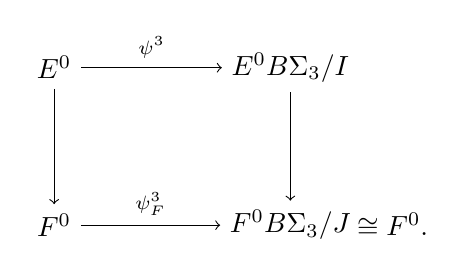
\begin{tikzpicture}
        \node (LT) at (0, 2) {$E^0$}; 
        \node (RT) at (3, 2) {$E^0 B\Sigma_3 / I$}; 
        \node (LB) at (0, 0) {$F^0$}; 
        \node (MB) at (3, 0) {$F^0 B\Sigma_3 / J$}; 
        \node (RB) at (4.3, 0) {$\cong F^0.  $}; 
        \draw [->] (LT) -- node [above] {$\scriptstyle \p$} (RT); 
        \draw [->] (LT) -- (LB); 
        \draw [->] (RT) -- (MB); 
        \draw [->] (LB) -- node [above] {$\scriptstyle \psi_F^3$} (MB); 
\end{tikzpicture}
\end{center}
Here $\psi_F^3$ is the $K(1)$-local power operation induced by $\p$, and 
$J \cong F^0 \otimes_{E^0} I$ is the transfer ideal.  Recall from 
Proposition \ref{prop:df}\thinspace \eqref{df(i)}, \eqref{strickland}, 
and Corollary \ref{cor:psi3} that $\p$ arises from the universal 
degree-3 isogeny which is parametrized by the ring $S_3$ with 
\[
 \big( S_3 \big)_{(3,h)}^\wedge \cong E^0 B\Sigma_3 / I.  
\]
The vertical maps are induced by the $K(1)$-localization $E \to F$.  In 
terms of homotopy groups, this is obtained by inverting the generator 
$h$ and completing at the prime 3 (see \cite[Corollary 1.5.5]{hovey97}): 
\[
 E_* = \BZ_9 \llbracket h \rrbracket [u^{\pm1}] \qquad \ad \qquad 
 F_* = \BZ_9 \llbracket h \rrbracket [h^{-1}]_3^\wedge [u^{\pm1}] 
\]
with 
\[
 F_0 = \BZ_9 (\!(h)\!)_3^\wedge = 
 \left.\left\{\sum_{n = -\infty}^{\infty} k_n h^n~\right|~k_n \in \BZ_9, 
 \lim_{n \to -\infty} k_n = 0\right\}.  
\]
The formal group $\HC$ over $E^0$ has a unique degree-3 subgroup after 
being pulled back to $F^0$, and the map 
\[
 E^0 B\Sigma_3 / I \to F^0 B\Sigma_3 / J \cong F^0 
\]
classifies this subgroup.  Along the base change 
\[
 E^0 B\Sigma_3 / I \to F^0 \otimes_{E^0} (E^0 B\Sigma_3 / I) 
 \cong (F^0 \otimes_{E^0} E^0 B\Sigma_3) / J \cong F^0 B\Sigma_3 / J, 
\]
the special fiber of the 3-divisible group of $\HC$ which consists 
solely of a formal component may split into formal and \'etale 
components (see Section \ref{subsec:fg}).  We want to take the formal 
component so as to keep track of the unique degree-3 subgroup of the 
formal group over $F^0$.  This subgroup gives rise to the $K(1)$-local 
power operation $\psi_F^3$.  

Recall from \eqref{S3} that $S_3 = S[\A] \big/ \big( w(\A) \big)$.  
Since 
\[
 w(\A) = \A^4 - 6 \A^2 + (h - 9) \A - 3 \equiv \A (\A^3 + h) \md 3, 
\]
the equation $w(\A) = 0$ has a unique root $\A = 0$ in $\BF_9 (\!(h)\!)$ 
(cf.~\eqref{Amod3}).  By Hensel's lemma this unique root lifts to a root 
in $\BZ_9 (\!(h)\!)_3^\wedge$; it corresponds to the unique degree-3 
subgroup of $\HC$ over $F^0$.  Plugging this specific value of $\A$ into 
the formulas for $\p$ in Corollary \ref{cor:psi3}, we then get an 
endomorphism of the ring $F^0$.  This endomorphism is the $K(1)$-local 
power operation $\psi_F^3$, and it determines the other $K(1)$-local 
power operations by iterated composition.  

Explicitly, with $h$ invertible in $F^0$, we solve for $\A$ from 
$w(\A) = 0$ by first writing 
\[
 \A = (3 + 6 \A^2 - \A^4) / (h - 9) 
 = (3 + 6 \A^2 - \A^4) \sum_{n = 1}^\infty 9^{n-1} h^{-n} 
\]
and then substituting this equation into itself recursively.  We plug 
the power series expansion for $\A$ into $\p(h)$ and get 
\[
 \psi_F^3(h) = h^3 - 27 h^2 + 183 h - 180 + 186 h^{-1} + 1674 h^{-2} 
 + (\text{lower-order terms}).  ~~~
\]
Similarly, writing $h$ as $c^2 + 1$ in $w(\A) = 0$, we solve for $\A$ in 
terms of $c$ and get 
\[
 \psi_F^3(c) = c^3 - 12 c - 6 c^{-1} - 84 c^{-3} - 933 c^{-5} 
 - 10956 c^{-7} + (\text{lower-order terms}).  
\]


\newpage
\appendix
\section*{Appendices}

Here we list long formulas whose appearance in the main body might 
affect readability.  The calculations involve power series expansions 
and manipulations of long polynomials with large coefficients (division, 
factorization, and finding greatest common divisors).  They are done 
using the software {\em Wolfram Mathematica 8}.  The commands 
\texttt{Reduce} and \texttt{Solve} are used to extract relations out of 
given identities.  


\section{Formulas in the proof of Proposition \ref{prop:tors}}
\label{apx:tors}

\begin{equation*}
\begin{split}
 \Tf(u) = & -\frac{u^4}{a^2 b} \big( b^4 u^8 + 3 a b^3 u^7 + 3 a^2 b^2 u^6 + (a^3 b + 7 a b^2) u^5 + (6 a^2 b - 6 b^2) u^4 \\
          & + 9 a b u^3 + (-a^2 + 8 b) u^2 - 3 a u - 3 \big), \\
 Q_1(v) = & ~ a b^2 v^2 + (b^2 d^2 + 2 a b d - b) v + \frac{b^2 d^4}{a} + 2 b d^3 + a d^2 - \frac{2 b d^2}{a} - d + \frac{1}{a}, \\
 R_1(v) = & ~ (\frac{b^3 d^6}{a} + 2 b^2 d^5 + a b d^4 - \frac{3 b^2 d^4}{a} + 2 b d^3 + \frac{3 b d^2}{a} - \frac{1}{a}) v + \frac{b^2 d^7}{a} + 2 b d^6 \\
          & + a d^5 - \frac{2 b d^5}{a} + 2 d^4 + \frac{d^3}{a}, \\
 Q_2(v) = & ~ \frac{a}{(b^3 d^6 + 2 a b^2 d^5 + a^2 b d^4 - 3 b^2 d^4 + 2 a b d^3 + 3 b d^2 - 1)^2} \big( (a b^4 d^6 + 2 a^2 b^3 d^5 \\
          & + a^3 b^2 d^4 - 3 a b^3 d^4 + 2 a^2 b^2 d^3 + 3 a b^2 d^2 - a b) v - b^4 d^8 - 2 a b^3 d^7 - a^2 b^2 d^6 \\
          & + 4 b^3 d^6 - a b^2 d^5 + a^2 b d^4 - 6 b^2 d^4 + 4 a b d^3 + 4 b d^2 - a d - 1 \big), \\
    R_2 = & - \frac{a d^4}{(b^3 d^6 + 2 a b^2 d^5 + a^2 b d^4 - 3 b^2 d^4 + 2 a b d^3 + 3 b d^2 - 1)^2} (b^4 d^8 + 3 a b^3 d^7 \\
          & + 3 a^2 b^2 d^6 + a^3 b d^5 + 7 a b^2 d^5 + 6 a^2 b d^4 - 6 b^2 d^4 + 9 a b d^3 - a^2 d^2 + 8 b d^2 \\
          & - 3 a d - 3), \\
   K(u) = & ~ \frac{b^3 u^6}{a} + 2 b^2 u^5 + (a b - \frac{3 b^2}{a}) u^4 + 2 b u^3 + \frac{3 b u^2}{a} - \frac{1}{a}, \\
   L(u) = & ~ \frac{b^2 u^7}{a} + 2 b u^6 + (a - \frac{2 b}{a}) u^5 + 2 u^4 + \frac{u^3}{a}, \\
   M(u) = & ~ \frac{b}{a^2 (a^2 - 16 b)^2} \big( (10 a^3 b^3 - 112 a b^4) u^5 + (19 a^4 b^2 - 217 a^2 b^3 - 16 b^4) u^4 \\
          & + (8 a^5 b - 126 a^3 b^2 + 304 a b^3) u^3 + (-a^6 + 34 a^4 b -266 a^2 b^2 +32 b^3) u^2 \\
          & + (28 a^3 b - 384 a b^2) u - 4 a^4 + 51 a^2 b - 16 b^2 \big), 
\end{split}
\end{equation*}
\begin{equation*}
\begin{split}
~  N(u) = & -\frac{1}{a (a^2 - 16 b)^2} \big( (10 a^3 b^5 - 112 a b^6) u^7 + (29 a^4 b^4 - 329 a^2 b^5 - 16 b^6) u^6 \\
          & + (27 a^5 b^3 - 313 a^3 b^4 - 48 a b^5 ) u^5 + (7 a^6 b^2 - 15 a^4 b^3 - 837 a^2 b^4 - 16 b^5) u^4 \\
          & + (-a^7 b + 66 a^5 b^2 - 714 a^3 b^3 + 528 a b^4) u^3 + (-4 a^6 b + 137 a^4 b^2 \\
          & - 1147 a^2 b^3 + 80 b^4) u^2 + (-12 a^5 b + 237 a^3 b^2 - 1200 a b^3) u + a^6 - 44 a^4 b \\
          & + 409 a^2 b^2 - 48 b^3 \big).  
\end{split}
\end{equation*}


\section{Formulas in the proof of Proposition \ref{prop:isog}}
\label{apx:isog}

The power series expansion of $v$ in terms of $u$ up to $u^{12}$ is 
\begin{equation*}
\begin{split}
 v = & ~ u^3 - a u^4 + (a^2 + b) u^5 + (-a^3 - 3 a b) u^6 + (a^4 + 6 a^2 b + b^2) u^7 + (-a^5 - 10 a^3 b \\
     & - 6 a b^2) u^8 + (a^6 + 15 a^4 b + 20 a^2 b^2 + b^3) u^9 + (-a^7 - 21 a^5 b - 50 a^3 b^2 \\
     & - 10 a b^3) u^{10} + (a^8 + 28 a^6 b + 105 a^4 b^2 + 50 a^2 b^3 + b^4) u^{11} + (-a^9 - 36 a^7 b \\
     & - 196 a^5 b^2 - 175 a^3 b^3 - 15 a b^4) u^{12}.  
\end{split}
\end{equation*}

Using the formulas of the group law on $C$ in Example \ref{ex:C}, we 
plug the coordinates of $P - Q$ and $P + Q$ into \eqref{u'v'}.  In view 
of \eqref{f}, we then have in \eqref{KL} 
\begin{equation*}
\begin{split}
      \K = & -\frac{1}{a^2 - 16 b} \big( a b^3 d^7 + (3 a^2 b^2 - 2 b^3) d^6 + (3 a^3 b - 6 a b^2) d^5 + (a^4 + a^2 b + 2 b^2) d^4 \\
           & + (4 a^3 - 15 a b) d^3 + (a^2 + 2 b) d^2 - 12 a d - 18 \big), \\
 \lambda = & -\frac{1}{a^2 b^2 (a^2 - 16 b)} \big( (a^3  b^3 - 11 a b^4) d^7 + (3 a^4 b^2 - 33 a^2 b^3 - 4 b^4) d^6 + (3 a^5 b \\
           & - 33 a^3 b^2 - 15 a b^3) d^5 + (a^6 - 4 a^4 b - 96 a^2 b^2 - 4 b^3) d^4 + (6 a^5 - 80 a^3 b \\
           & + 31 a b^2) d^3 + (10 a^4 - 153 a^2 b + 20 b^2) d^2 + (3 a^3 - 117 a b) d - 6 a^2 - 12 b \big).  
\end{split}
\end{equation*}
More extended power series expansions in $u$ for $u'$ (up to $u^6$) and 
$v'$ (up to $u^9$) are needed in \eqref{KL} to determine the 
coefficients in the equation of $C'$: 
\begin{equation*}
\begin{split}
     u' = & -\frac{1}{a^2 - 16 b} \big( (a b^3 d^7 + 3 a^2 b^2 d^6 - 2 b^3 d^6 + 3 a^3 b d^5 - 6 a b^2 d^5 + a^4 d^4 + a^2 b d^4 \\
          & + 2 b^2 d^4 + 4 a^3 d^3 - 15 a b d^3 + a^2 d^2 + 2 b d^2 - 12 a d - 18) u + (-a^2 b^3 d^7 \\
          & + 12 b^4 d^7 - 3 a^3 b^2 d^6 + 36 a b^3 d^6 - 3 a^4 b d^5 + 36 a^2 b^2 d^5 + 4 b^3 d^5 - a^5 d^4 \\
          & + 5 a^3 b d^4 + 94 a b^2 d^4 - 6 a^4 d^3 + 85 a^2 b d^3 - 76 b^2 d^3 - 9 a^3 d^2 + 136 a b d^2 + 60 b d \\
          & + 6 a) u^2 + (a^3 b^3 d^7 - 17 a b^4 d^7 + 3 a^4 b^2 d^6 - 50 a^2 b^3 d^6 - 8 b^4 d^6 + 3 a^5 b d^5 
\end{split}
\end{equation*}
\begin{equation*}
\begin{split}
          & - 48 a^3 b^2 d^5 - 27 a b^3 d^5 + a^6 d^4 - 7 a^4 b d^4 - 150 a^2 b^2 d^4 - 16 b^3 d^4 + 7 a^5 d^3 \\
          & - 113 a^3 b d^3 + 9 a b^2 d^3 + 16 a^4 d^2 - 258 a^2 b d^2 + 56 b^2 d^2 + 15 a^3 d - 237 a b d \\
          & + 2 a^2 - 32 b) u^3 + (-a^4 b^3 d^7 + 16 a^2 b^4 d^7 + 12 b^5 d^7 - 3 a^5 b^2 d^6 + 46 a^3 b^3 d^6 \\
          & + 64 a b^4 d^6 - 3 a^6 b d^5 + 42 a^4 b^2 d^5 + 121 a^2 b^3 d^5 + 4 b^4 d^5 - a^7 d^4 + 3 a^5 b d^4 \\
          & + 209 a^3 b^2 d^4 + 122 a b^3 d^4 - 8 a^6 d^3 + 114 a^4 b d^3 + 248 a^2 b^2 d^3 - 76 b^3 d^3 \\
          & - 24 a^5 d^2 + 384 a^3 b d^2 - 4 a b^2 d^2 - 33 a^4 d + 519 a^2 b d + 60 b^2 d - 18 a^3 \\
          & + 282 a b) u^4 + (a^5 b^3 d^7 - 9 a^3 b^4 d^7 - 117 a b^5 d^7 + 3 a^6 b^2 d^6 - 24 a^4 b^3 d^6 \\
          & - 396 a^2 b^4 d^6 - 24 b^5 d^6 + 3 a^7 b d^5 - 18 a^5 b^2 d^5 - 484 a^3 b^3 d^5 - 111 a b^4 d^5 + a^8 d^4 \\
          & + 7 a^6 b d^4 - 307 a^4 b^2 d^4 - 1038 a^2 b^3 d^4 + 9 a^7 d^3 - 73 a^5 b d^3 - 1181 a^3 b^2 d^3 \\
          & + 573 a b^3 d^3 + 33 a^6 d^2 - 451 a^4 b d^2 - 1236 a^2 b^2 d^2 + 72 b^3 d^2 + 54 a^5 d \\
          & - 807 a^3 b d - 873 a b^2 d + 36 a^4 - 570 a^2 b - 48 b^2) u^5 + (-a^6 b^3 d^7 - 5 a^4 b^4 d^7 \\
          & + 337 a^2 b^5 d^7 + 12 b^6 d^7 - 3 a^7 b^2 d^6 - 19 a^5 b^3 d^6 + 1064 a^3 b^4 d^6 + 204 a b^5 d^6 \\
          & - 3 a^8 b d^5 - 27 a^6 b^2 d^5 + 1164 a^4 b^3 d^5 + 638 a^2 b^4 d^5 + 4 b^5 d^5 - a^9 d^4 - 24 a^7 b d^4 \\
          & + 441 a^5 b^2 d^4 + 3195 a^3 b^3 d^4 + 182 a b^4 d^4 - 10 a^8 d^3 - 22 a^6 b d^3 + 2956 a^4 b^2 d^3 \\
          & - 645 a^2 b^3 d^3 - 76 b^4 d^3 - 43 a^7 d^2 + 403 a^5 b d^2 + 4594 a^3 b^2 d^2 - 544 a b^3 d^2 \\
          & - 78 a^6 d + 996 a^4 b d + 4014 a^2 b^2 d + 60 b^3 d - 57 a^5 + 852 a^3 b + 942 a b^2) u^6 \big), \\
     v' = & -\frac{1}{a^2 b^2 (a^2 - 16 b)} \big( (a^3 b^3 d^7 - 11 a b^4 d^7 + 3 a^4 b^2 d^6 - 33 a^2 b^3 d^6 - 4 b^4 d^6 \\
          & + 3 a^5 b d^5 - 33 a^3 b^2 d^5 - 15 a b^3 d^5 + a^6 d^4 - 4 a^4 b d^4 - 96 a^2 b^2 d^4 - 4 b^3 d^4 \\
          & + 6 a^5 d^3 - 80 a^3 b d^3 + 31 a b^2 d^3 + 10 a^4 d^2 - 153 a^2 b d^2 + 20 b^2 d^2 + 3 a^3 d \\
          & - 117 a b d - 6 a^2 - 12 b) u^3 + (-2 a^4 b^3 d^7 + 28 a^2 b^4 d^7 - 6 a^5 b^2 d^6 + 82 a^3 b^3 d^6 \\
          & + 28 a b^4 d^6 - 6 a^6 b d^5 + 78 a^4 b^2 d^5 + 90 a^2 b^3 d^5 - 2 a^7 d^4 + 8 a^5 b d^4 + 294 a^3 b^2 d^4 \\
          & + 20 a b^3 d^4 - 14 a^6 d^3 + 202 a^4 b d^3 + 72 a^2 b^2 d^3 - 32 a^5 d^2 + 510 a^3 b d^2 \\
          & - 124 a b^2 d^2 - 30 a^4 d + 546 a^2 b d - 6 a^3 + 204 a b) u^4 + (3 a^5 b^3 d^7 - 38 a^3 b^4 d^7 \\
          & - 107 a b^5 d^7 + 9 a^6 b^2 d^6 - 108 a^4 b^3 d^6 - 409 a^2 b^4 d^6 - 4 b^5 d^6 + 9 a^7 b d^5 \\
          & - 96 a^5 b^2 d^5 - 590 a^3 b^3 d^5 - 47 a b^4 d^5 + 3 a^8 d^4 + a^6 b d^4 - 646 a^4 b^2 d^4 \\
          & - 912 a^2 b^3 d^4 - 4 b^4 d^4 + 24 a^7 d^3 - 292 a^5 b d^3 - 1249 a^3 b^2 d^3 + 639 a b^3 d^3 \\
          & + 70 a^6 d^2 - 1057 a^4 b d^2 - 849 a^2 b^2 d^2 + 20 b^3 d^2 + 93 a^5 d - 1512 a^3 b d \\
          & - 597 a b^2 d + 48 a^4 - 870 a^2 b - 12 b^2) u^5 + (-4 a^6 b^3 d^7 + 24 a^4 b^4 d^7 + 583 a^2 b^5 d^7 \\
          & - 12 a^7 b^2 d^6 + 60 a^5 b^3 d^6 + 1923 a^3 b^4 d^6 + 156 a b^5 d^6 - 12 a^8 b d^5 + 36 a^6 b^2 d^5 \\
          & + 2268 a^4 b^3 d^5 + 639 a^2 b^4 d^5 - 4 a^9 d^4 - 40 a^7 b d^4 + 1256 a^5 b^2 d^4 + 5128 a^3 b^3 d^4 
\end{split}
\end{equation*}
\begin{equation*}
\begin{split}
\quad ~~~ & + 140 a b^4 d^4 - 36 a^8 d^3 + 229 a^6 b d^3 + 5409 a^4 b^2 d^3 - 2227 a^2 b^3 d^3 - 127 a^7 d^2 \\
          & + 1597 a^5 b d^2 + 6835 a^3 b^2 d^2 - 748 a b^3 d^2 - 201 a^6 d + 2952 a^4 b d + 5277 a^2 b^2 d \\
          & - 129 a^5 + 2130 a^3 b + 708 a b^2) u^6 + (5 a^7 b^3 d^7 + 35 a^5 b^4 d^7 - 1754 a^3 b^5 d^7 \\
          & - 275 a b^6 d^7 + 15 a^8 b^2 d^6 + 125 a^6 b^3 d^6 - 5511 a^4 b^4 d^6 - 1833 a^2 b^5 d^6 - 4 b^6 d^6 \\
          & + 15 a^9 b d^5 + 165 a^7 b^2 d^5 - 5988 a^5 b^3 d^5 - 4312 a^3 b^4 d^5 - 103 a b^5 d^5 + 5 a^{10} d^4 \\
          & + 130 a^8 b d^4 - 2183 a^6 b^2 d^4 - 17022 a^4 b^3 d^4 - 2940 a^2 b^4 d^4 - 4 b^5 d^4 + 50 a^9 d^3 \\
          & + 159 a^7 b d^3 - 15035 a^5 b^2 d^3 + 179 a^3 b^3 d^3 + 1703 a b^4 d^3 + 206 a^8 d^2 \\
          & - 1708 a^6 b d^2 - 25304 a^4 b^2 d^2 + 1431 a^2 b^3 d^2 + 20 b^4 d^2 + 363 a^7 d - 4398 a^5 b d \\
          & - 23694 a^3 b^2 d - 1437 a b^3 d + 258 a^6 - 3816 a^4 b - 7026 a^2 b^2 - 12 b^3) u^7 \\
          & + (-6 a^8 b^3 d^7 - 164 a^6 b^4 d^7 + 3864 a^4 b^5 d^7 + 3365 a^2 b^6 d^7 - 18 a^9 b^2 d^6 \\
          & - 522 a^7 b^3 d^6 + 11837 a^5 b^4 d^6 + 13701 a^3 b^5 d^6 + 448 a b^6 d^6 - 18 a^{10} b d^5 \\
          & - 582 a^8 b^2 d^5 + 12275 a^6 b^3 d^5 + 21828 a^4 b^4 d^5 + 2395 a^2 b^5 d^5 - 6 a^{11} d^4 \\
          & - 296 a^9 b d^4 + 3283 a^7 b^2 d^4 + 43960 a^5 b^3 d^4 + 30290 a^3 b^4 d^4 + 424 a b^5 d^4 \\
          & - 66 a^{10} d^3 - 1099 a^8 b d^3 + 32246 a^6 b^2 d^3 + 30529 a^4 b^3 d^3 - 17045 a^2 b^4 d^3 \\
          & - 310 a^9 d^2 + 679 a^7 b d^2 + 66726 a^5 b^2 d^2 + 24833 a^3 b^3 d^2 - 2192 a b^4 d^2 - 588 a^8 d \\
          & + 4809 a^6 b d + 73578 a^4 b^2 d + 23685 a^2 b^3 d - 444 a^7 + 5316 a^5 b + 30936 a^3 b^2 \\
          & + 1704 a b^3) u^8 + (7 a^9 b^3 d^7 + 392 a^7 b^4 d^7 - 6863 a^5 b^5 d^7 - 17458 a^3 b^6 d^7 \\
          & - 515 a b^7 d^7 + 21 a^{10} b^2 d^6 + 1218 a^8 b^3 d^6 - 20647 a^6 b^4 d^6 - 61745 a^4 b^5 d^6 \\
          & - 6709 a^2 b^6 d^6 - 4 b^7 d^6 + 21 a^{11} b d^5 + 1302 a^9 b^2 d^5 - 20664 a^7 b^3 d^5 \\
          & - 81924 a^5 b^4 d^5 - 22146 a^3 b^5 d^5 - 183 a b^6 d^5 + 7 a^{12} d^4 + 567 a^{10} b d^4 \\
          & - 3982 a^8 b^2 d^4 - 97733 a^6 b^3 d^4 - 158644 a^4 b^4 d^4 - 8392 a^2 b^5 d^4 - 4 b^6 d^4 \\
          & + 84 a^{11} d^3 + 2878 a^9 b d^3 - 57242 a^7 b^2 d^3 - 160981 a^5 b^3 d^3 + 59447 a^3 b^4 d^3 \\
          & + 3223 a b^5 d^3 + 442 a^{10} d^2 + 2563 a^8 b d^2 - 142138 a^6 b^2 d^2 - 189134 a^4 b^3 d^2 \\
          & + 18323 a^2 b^4 d^2 + 20 b^5 d^2 + 885 a^9 d - 2382 a^7 b d - 179958 a^5 b^2 d \\
          & - 164688 a^3 b^3 d - 2637 a b^4 d + 696 a^8 - 5400 a^6 b - 92938 a^4 b^2 - 29078 a^2 b^3 \\
          & - 12 b^4) u^9 \big).  
\end{split}
\end{equation*}

%\nocite{*}
%\bibliographystyle{amsalpha}
%\bibliography{draft}
%\end{document}

\newpage
\newcommand{\MRn}[2]{\href{http://www.ams.org/mathscinet-getitem?mr=#1}{MR#1 #2}}
\begin{thebibliography}

\bibitem[Ada60]{adamshopf}
J.~F. Adams, \emph{On the non-existence of elements of {H}opf invariant one},
  Ann. of Math. (2) \textbf{72} (1960), 20--104. \MRn{0141119}{(25 \#4530)}

\bibitem[Ada62]{adamsvector}
\bysame, \emph{Vector fields on spheres}, Ann. of Math. (2) \textbf{75} (1962),
  603--632. \MRn{0139178}{(25 \#2614)}

\bibitem[Ada74]{sh}
\bysame, \emph{Stable homotopy and generalised homology}, University of Chicago
  Press, Chicago, Ill., 1974, Chicago Lectures in Mathematics. \MRn{0402720}{(53
  \#6534)}

\bibitem[Ade52]{adem}
Jos{\'e} Adem, \emph{The iteration of the {S}teenrod squares in algebraic
  topology}, Proc. Nat. Acad. Sci. U. S. A. \textbf{38} (1952), 720--726.
  \MRn{0050278}{(14,306e)}

\bibitem[AHS01]{AHS01}
M.~Ando, M.~J. Hopkins, and N.~P. Strickland, \emph{Elliptic spectra, the
  {W}itten genus and the theorem of the cube}, Invent. Math. \textbf{146}
  (2001), no.~3, 595--687. \MRn{1869850}{(2002g:55009)}

\bibitem[AHS04]{AHS04}
Matthew Ando, Michael~J. Hopkins, and Neil~P. Strickland, \emph{The sigma
  orientation is an {$H\sb \infty$} map}, Amer. J. Math. \textbf{126} (2004),
  no.~2, 247--334. \MRn{2045503}{(2005d:55009)}

\bibitem[AL70]{atkinlehner}
A.~O.~L. Atkin and J.~Lehner, \emph{Hecke operators on {$\Gamma \sb{0}(m)$}},
  Math. Ann. \textbf{185} (1970), 134--160. \MRn{0268123}{(42 \#3022)}

\bibitem[And95]{Ando95}
Matthew Ando, \emph{Isogenies of formal group laws and power operations in the
  cohomology theories {$E\sb n$}}, Duke Math. J. \textbf{79} (1995), no.~2,
  423--485. \MRn{1344767}{(97a:55006)}

\bibitem[And00]{Ando00}
\bysame, \emph{Power operations in elliptic cohomology and representations of
  loop groups}, Trans. Amer. Math. Soc. \textbf{352} (2000), no.~12,
  5619--5666. \MRn{1637129}{(2001b:55016)}

\bibitem[AS69]{atiyahsegal}
M.~F. Atiyah and G.~B. Segal, \emph{Equivariant {$K$}-theory and completion},
  J. Differential Geometry \textbf{3} (1969), 1--18. \MRn{0259946}{(41 \#4575)}

\bibitem[Ati66]{atiyah}
M.~F. Atiyah, \emph{Power operations in {$K$}-theory}, Quart. J. Math. Oxford
  Ser. (2) \textbf{17} (1966), 165--193. \MRn{0202130}{(34 \#2004)}

\bibitem[BGJGP05]{poonen}
Matthew~H. Baker, Enrique Gonz{\'a}lez-Jim{\'e}nez, Josep Gonz{\'a}lez, and
  Bjorn Poonen, \emph{Finiteness results for modular curves of genus at least
  2}, Amer. J. Math. \textbf{127} (2005), no.~6, 1325--1387. \MRn{2183527}{(2006i:11065)}

\bibitem[BMMS86]{H_infty}
R.~R. Bruner, J.~P. May, J.~E. McClure, and M.~Steinberger, \emph{{$H\sb \infty
  $} ring spectra and their applications}, Lecture Notes in Mathematics, vol.
  1176, Springer-Verlag, Berlin, 1986. \MRn{836132}{(88e:55001)}

\bibitem[Bor94]{borceux}
Francis Borceux, \emph{Handbook of categorical algebra. 2}, Encyclopedia of
  Mathematics and its Applications, vol.~51, Cambridge University Press,
  Cambridge, 1994, Categories and structures. \MRn{1313497}{(96g:18001b)}

\bibitem[Bou79]{bousfield}
A.~K. Bousfield, \emph{The localization of spectra with respect to homology},
  Topology \textbf{18} (1979), no.~4, 257--281. \MRn{551009}{(80m:55006)}

\bibitem[Car54]{cartan}
Henri Cartan, \emph{Sur les groupes d'{E}ilenberg-{M}ac {L}ane. {II}}, Proc.
  Nat. Acad. Sci. U. S. A. \textbf{40} (1954), 704--707. \MRn{0065161}{(16,390b)}

\bibitem[Dew99]{dewaghe}
L.~Dewaghe, \emph{Isog\'enie entre courbes elliptiques}, Util. Math.
  \textbf{55} (1999), 123--127. \MRn{1685678}{(2000b:14034)}

\bibitem[EKMM97]{EKMM}
A.~D. Elmendorf, I.~Kriz, M.~A. Mandell, and J.~P. May, \emph{Rings, modules,
  and algebras in stable homotopy theory}, Mathematical Surveys and Monographs,
  vol.~47, American Mathematical Society, Providence, RI, 1997, With an
  appendix by M. Cole. \MRn{1417719}{(97h:55006)}

\bibitem[Gan]{ganter}
Nora Ganter, \emph{Stringy power operations in {T}ate ${K}$-theory}, preprint,
  available at \href{http://arxiv.org/abs/math/0701565}{arXiv:0701565}.

\bibitem[GH04]{goersshopkins}
P.~G. Goerss and M.~J. Hopkins, \emph{Moduli spaces of commutative ring
  spectra}, Structured ring spectra, London Math. Soc. Lecture Note Ser., vol.
  315, Cambridge Univ. Press, Cambridge, 2004, pp.~151--200. \MRn{2125040}{(2006b:55010)}

\bibitem[Gre88]{blind}
J.~P.~C. Greenlees, \emph{How blind is your favourite cohomology theory?},
  Exposition. Math. \textbf{6} (1988), no.~3, 193--208. \MRn{949783}{(89j:55001)}

\bibitem[HM]{hopkinsmahowald}
Mike Hopkins and Mark Mahowald, \emph{From elliptic curves to homotopy theory},
  preprint, available at
  \href{http://hopf.math.purdue.edu//Hopkins-Mahowald/eo2homotopy.pdf}{http://hopf.math.purdue.edu//Hopkins-Mahowald/eo2homotopy.pdf}.

\bibitem[Hopa]{hopkins}
M.~J. Hopkins, \emph{{$K(1)$}-local {$E\sb \infty $} ring spectra}, unpublished
  notes, available at 
  \href{http://www.math.rochester.edu/people/faculty/doug/otherpapers/knlocal.pdf}{http://\linebreak www.math.rochester.edu/people/faculty/doug/otherpapers/knlocal.pdf}.

\bibitem[Hopb]{coctalos}
Mike Hopkins, \emph{Complex oriented cohomology theories and the language of
  stacks}, course notes, available at 
  \href{http://www.math.rochester.edu/people/faculty/doug/otherpapers/coctalos.pdf}{http://www.math.rochester.edu/people/faculty/doug/\linebreak otherpapers/coctalos.pdf}.

\bibitem[Hov97]{hovey97}
Mark~A. Hovey, \emph{{$v\sb n$}-{E}lements in ring spectra and applications to
  bordism theory}, Duke Math. J. \textbf{88} (1997), no.~2, 327--356.
  \MRn{1455523}{(98d:55017)}

\bibitem[Hov08]{hovey08}
Mark Hovey, \emph{Morava {$E$}-theory of filtered colimits}, Trans. Amer. Math.
  Soc. \textbf{360} (2008), no.~1, 369--382 (electronic). \MRn{2342007}{(2008g:55007)}

\bibitem[HS99]{hoveystrickland}
Mark Hovey and Neil~P. Strickland, \emph{Morava {$K$}-theories and
  localisation}, Mem. Amer. Math. Soc. \textbf{139} (1999), no.~666, viii+100.
  \MRn{1601906}{(99b:55017)}

\bibitem[Hus04]{husemoller}
Dale Husem{\"o}ller, \emph{Elliptic curves}, second ed., Graduate Texts in
  Mathematics, vol. 111, Springer-Verlag, New York, 2004, With appendices by
  Otto Forster, Ruth Lawrence and Stefan Theisen. \MRn{2024529}{(2005a:11078)}

\bibitem[KM85]{KM}
Nicholas~M. Katz and Barry Mazur, \emph{Arithmetic moduli of elliptic curves},
  Annals of Mathematics Studies, vol. 108, Princeton University Press,
  Princeton, NJ, 1985. \MRn{772569}{(86i:11024)}

\bibitem[Koh96]{kohel}
David~Russell Kohel, \emph{Endomorphism rings of elliptic curves over finite
  fields}, ProQuest LLC, Ann Arbor, MI, 1996, Thesis (Ph.D.)--University of
  California, Berkeley. \MRn{2695524}{}

\bibitem[Law63]{lawvere}
F.~William Lawvere, \emph{Functorial semantics of algebraic theories}, Proc.
  Nat. Acad. Sci. U.S.A. \textbf{50} (1963), 869--872. \MRn{0158921}{(28 \#2143)}

\bibitem[Law09]{tafoverview}
Tyler Lawson, \emph{An overview of abelian varieties in homotopy theory}, New
  topological contexts for {G}alois theory and algebraic geometry ({BIRS}
  2008), Geom. Topol. Monogr., vol.~16, Geom. Topol. Publ., Coventry, 2009,
  pp.~179--214. \MRn{2544390}{(2010i:55006)}

\bibitem[LN12]{level3}
Tyler Lawson and Niko Naumann, \emph{Commutativity conditions for truncated
  {B}rown-{P}eterson spectra of height 2}, J. Topol. \textbf{5} (2012), no.~1,
  137--168. \MRn{2897051}{}

\bibitem[LT66]{lubintate}
Jonathan Lubin and John Tate, \emph{Formal moduli for one-parameter formal
  {L}ie groups}, Bull. Soc. Math. France \textbf{94} (1966), 49--59.
  \MRn{0238854}{(39 \#214)}

\bibitem[Lub67]{lubin}
Jonathan Lubin, \emph{Finite subgroups and isogenies of one-parameter formal
  {L}ie groups}, Ann. of Math. (2) \textbf{85} (1967), 296--302. \MRn{0209287}{(35 \#189)}

\bibitem[Lur]{252x}
Jacob Lurie, \emph{Chromatic homotopy theory}, course notes, available at
  \href{http://www.math.harvard.edu/~lurie/252x.html}{http://www.\linebreak math.harvard.edu/\textasciitilde
  lurie/252x.html}.

\bibitem[Lur09]{survey}
J.~Lurie, \emph{A survey of elliptic cohomology}, Algebraic topology, Abel
  Symp., vol.~4, Springer, Berlin, 2009, pp.~219--277. \MRn{2597740}{(2011f:55009)}

\bibitem[McC83]{mcclure}
James~E. McClure, \emph{Dyer-{L}ashof operations in {$K$}-theory}, Bull. Amer.
  Math. Soc. (N.S.) \textbf{8} (1983), no.~1, 67--72. \MRn{682824}{(84e:55014)}

\bibitem[MFK94]{GIT}
D.~Mumford, J.~Fogarty, and F.~Kirwan, \emph{Geometric invariant theory}, third
  ed., Ergebnisse der Mathematik und ihrer Grenzgebiete (2) [Results in
  Mathematics and Related Areas (2)], vol.~34, Springer-Verlag, Berlin, 1994.
  \MRn{1304906}{(95m:14012)}

\bibitem[Mil58]{milnor}
John Milnor, \emph{The {S}teenrod algebra and its dual}, Ann. of Math. (2)
  \textbf{67} (1958), 150--171. \MRn{0099653}{(20 \#6092)}

\bibitem[Mor89]{morava}
Jack Morava, \emph{Forms of {$K$}-theory}, Math. Z. \textbf{201} (1989), no.~3,
  401--428. \MRn{999737}{(90e:55011)}

\bibitem[MR09]{tmf3}
Mark Mahowald and Charles Rezk, \emph{Topological modular forms of level 3},
  Pure Appl. Math. Q. \textbf{5} (2009), no.~2, Special Issue: In honor of
  Friedrich Hirzebruch. Part 1, 853--872. \MRn{2508904}{(2010g:55010)}

\bibitem[MT68]{moshertangora}
Robert~E. Mosher and Martin~C. Tangora, \emph{Cohomology operations and
  applications in homotopy theory}, Harper \& Row Publishers, New York, 1968.
  \MRn{0226634}{(37 \#2223)}

\bibitem[Pea]{pearson}
Paul Pearson, \emph{Calculating formal group laws}, unpublished notes,
  available at
  \href{http://www.math.rochester.edu/people/faculty/pearson/papers/fgls-2up.pdf}{http://\linebreak www.math.rochester.edu/people/faculty/pearson/papers/fgls-2up.pdf}.

\bibitem[Qui69]{quillenfgl}
Daniel Quillen, \emph{On the formal group laws of unoriented and complex
  cobordism theory}, Bull. Amer. Math. Soc. \textbf{75} (1969), 1293--1298.
  \MRn{0253350}{(40 \#6565)}

\bibitem[Qui71]{quillenmu}
\bysame, \emph{Elementary proofs of some results of cobordism theory using
  {S}teenrod operations}, Advances in Math. \textbf{7} (1971), 29--56 (1971).
  \MRn{0290382}{(44 \#7566)}

\bibitem[Rav92]{orange}
Douglas~C. Ravenel, \emph{Nilpotence and periodicity in stable homotopy
  theory}, Annals of Mathematics Studies, vol. 128, Princeton University Press,
  Princeton, NJ, 1992, Appendix C by Jeff Smith. \MRn{1192553}{(94b:55015)}

\bibitem[Reza]{lpo}
Charles Rezk, \emph{Lectures on power operations}, course notes, available at
  \href{http://www.math.uiuc.edu/~rezk/power-operation-lectures.dvi}{http://www.\linebreak math.uiuc.edu/\textasciitilde
  rezk/power-operation-lectures.dvi}.

\bibitem[Rezb]{h2p2}
\bysame, \emph{Power operations for {M}orava ${E}$-theory of height 2 at the
  prime 2}, preprint, available at
  \href{http://arxiv.org/abs/0812.1320}{arXiv:0812.1320}.

\bibitem[Rezc]{slides}
\bysame, \emph{Power operations in {M}orava ${E}$-theory: a survey}, slides for
  a talk at the Midwest Topology Seminar (Minneapolis, MN, 2009), available at
  \href{http://www.math.uiuc.edu/~rezk/midwest-2009-power-ops-handout.pdf}{http://www.\linebreak math.uiuc.edu/\textasciitilde
  rezk/midwest-2009-power-ops-handout.pdf}.

\bibitem[Rezd]{koszul}
\bysame, \emph{Rings of power operations for {M}orava ${E}$-theories are
  {K}oszul}, preprint, available at
  \href{http://arxiv.org/abs/1204.4831}{arXiv:1204.4831}.

\bibitem[Rez98]{Rnotes}
\bysame, \emph{Notes on the {H}opkins-{M}iller theorem}, Homotopy theory via
  algebraic geometry and group representations ({E}vanston, {IL}, 1997),
  Contemp. Math., vol. 220, Amer. Math. Soc., Providence, RI, 1998,
  pp.~313--366. \MRn{1642902}{(2000i:55023)}

\bibitem[Rez09]{cong}
\bysame, \emph{The congruence criterion for power operations in {M}orava
  {$E$}-theory}, Homology, Homotopy Appl. \textbf{11} (2009), no.~2, 327--379.
  \MRn{2591924}{(2011e:55021)}

\bibitem[Seg68]{segal}
Graeme Segal, \emph{Equivariant {$K$}-theory}, Inst. Hautes \'Etudes Sci. Publ.
  Math. (1968), no.~34, 129--151. \MRn{0234452}{(38 \#2769)}

\bibitem[Ser53]{serre}
Jean-Pierre Serre, \emph{Cohomologie modulo {$2$} des complexes
  d'{E}ilenberg-{M}ac{L}ane}, Comment. Math. Helv. \textbf{27} (1953),
  198--232. \MRn{0060234}{(15,643c)}

\bibitem[Sil94]{AECII}
Joseph~H. Silverman, \emph{Advanced topics in the arithmetic of elliptic
  curves}, Graduate Texts in Mathematics, vol. 151, Springer-Verlag, New York,
  1994. \MRn{1312368}{(96b:11074)}

\bibitem[Sil09]{AEC}
\bysame, \emph{The arithmetic of elliptic curves}, second ed., Graduate Texts
  in Mathematics, vol. 106, Springer, Dordrecht, 2009. \MRn{2514094}{(2010i:11005)}

\bibitem[Ste62]{steenrod}
N.~E. Steenrod, \emph{Cohomology operations}, Lectures by N. E. Steenrod
  written and revised by D. B. A. Epstein. Annals of Mathematics Studies, No.
  50, Princeton University Press, Princeton, N.J., 1962. \MRn{0145525}{(26
  \#3056)}

\bibitem[Str97]{Str97}
Neil~P. Strickland, \emph{Finite subgroups of formal groups}, J. Pure Appl.
  Algebra \textbf{121} (1997), no.~2, 161--208. \MRn{1473889}{(98k:14065)}

\bibitem[Str98]{Str98}
N.~P. Strickland, \emph{Morava {$E$}-theory of symmetric groups}, Topology
  \textbf{37} (1998), no.~4, 757--779. \MRn{1607736}{(99e:55008)}

\bibitem[SW51]{steenrodwhitehead}
N.~E. Steenrod and J.~H.~C. Whitehead, \emph{Vector fields on the
  {$n$}-sphere}, Proc. Nat. Acad. Sci. U. S. A. \textbf{37} (1951), 58--63.
  \MRn{0041436}{(12,847c)}

\bibitem[Tat67]{tate}
J.~T. Tate, \emph{{$p$}-{D}ivisible groups}, Proc. {C}onf. {L}ocal {F}ields
  ({D}riebergen, 1966), Springer, Berlin, 1967, pp.~158--183. \MRn{0231827}{(38
  \#155)}

\bibitem[tD68]{tomdieck}
Tammo tom Dieck, \emph{Steenrod-{O}perationen in {K}obordismen-{T}heorien},
  Math. Z. \textbf{107} (1968), 380--401. \MRn{0244989}{(39 \#6302)}

\bibitem[TO70]{tateoort}
John Tate and Frans Oort, \emph{Group schemes of prime order}, Ann. Sci.
  \'Ecole Norm. Sup. (4) \textbf{3} (1970), 1--21. \MRn{0265368}{(42 \#278)}

\bibitem[V{\'e}l71]{velu}
Jacques V{\'e}lu, \emph{Isog\'enies entre courbes elliptiques}, C. R. Acad.
  Sci. Paris S\'er. A-B \textbf{273} (1971), A238--A241. \MRn{0294345}{(45
  \#3414)}

\bibitem[Voe03]{V}
Vladimir Voevodsky, \emph{Reduced power operations in motivic cohomology},
  Publ. Math. Inst. Hautes \'Etudes Sci. (2003), no.~98, 1--57. \MRn{2031198}{(2005b:14038a)}

\bibitem[Wah01]{wahl}
Nathalie Wahl, \emph{Ribbon {B}raids and related operads}, Thesis
  (Ph.D.)--University of Oxford, 2001, available at
  \href{http://www.math.ku.dk/~wahl/wahlthesis.ps}{http://www.math.ku.dk/\textasciitilde
  wahl/wahlthesis.ps}.

\bibitem[Wil82]{wilkerson}
Clarence Wilkerson, \emph{Lambda-rings, binomial domains, and vector bundles
  over {${\bf C}P(\infty )$}}, Comm. Algebra \textbf{10} (1982), no.~3,
  311--328. \MRn{651605}{(83f:55003)}

\end{thebibliography}
\end{document}